\documentclass[12pt, twoside, openany]{book}

% !TEX root=../../mt-motion-analysis.tex
\usepackage[citestyle=ieee, bibstyle=ieee, style=numeric-comp, sorting=nty, maxbibnames=99]{biblatex}

\usepackage[utf8]{inputenc}

% Makes the last name first in the bibliography.
% \DeclareNameAlias{author}{last-first}
% \DeclareNameAlias{author}{family-given}

% Specify the margins. This is 6.25inches in text with which
% can be used to size figures to the correct size.
\usepackage[a4paper, margin=2.5625cm]{geometry}


\usepackage{eso-pic}					% Packages for layout and graphics
\usepackage{graphicx}
\usepackage{tikz}
\usetikzlibrary{fadings}
\usepackage{setspace}
% \usepackage{tocloft}		 			% Fixing a bug with page style changes for toc
% \tocloftpagestyle{plain}
\usepackage{etoc} 						% Separate tocs for appendix and the rest
\usepackage{chngcntr}					% Count figures within chapters
\usepackage{booktabs}					% Table formatting
\usepackage{fancyhdr}					% Setting the style for header and footer.
\usepackage{tabularx}
\usepackage{multirow}                   % For better tables
\usepackage[hidelinks]{hyperref}		% Clickable links
\usepackage{nameref}					% References with names
\usepackage[parfill]{parskip}			% New line instead of indent for sections
\usepackage{tcolorbox}					% Create boxes around content
\tcbset{colback=white,arc=0mm}

\usepackage{amsmath}
\usepackage{mathdots}
\usepackage{yhmath}
\usepackage{siunitx}
\usepackage{array}
\usepackage{gensymb}
\usepackage{amssymb}
\usepackage{mathtools}              % Add text to math arrows.

\usepackage{cancel}
\usepackage{color}
\usepackage{multirow}
\usepackage{textcomp}               % Fixing warning for gensyb \perthousand
\usepackage{svg}                    % including svg files
\usepackage{caption}                % For subfigures
\usepackage{subcaption}
\usepackage{fontspec}
\usepackage{sectsty}
\usepackage{tocloft}

\usepackage[printonlyused]{acronym}

\usepackage{slashbox}
\usepackage{arydshln}

\usepackage{cleveref}

\usepackage{unicode-math}

% \usepackage{bm}

\usepackage[acronym, nonumberlist, nopostdot, xindy, nomain, nogroupskip]{glossaries}





\counterwithin{figure}{section}
\counterwithin{table}{section}

% Specifying fonts
% \setmainfont{Georgia}
% \setsansfont{Arial}
% \newfontfamily\footerfont{Georgia}

\chapterfont{\sffamily\fontsize{17}{17}}
\sectionfont{\sffamily\fontsize{14}{15}}
\subsectionfont{\sffamily\fontsize{13}{15}}
\subsubsectionfont{\sffamily\fontsize{12}{15}}

% Remove the title and make sure that the text is adjusted
% \usepackage{abstract}
% \setlength{\absleftindent}{0mm}
% \renewcommand{\abstractname}{\vspace{-\baselineskip}}
% \renewcommand{\abstractnamefont}{\sffamily\fontsize{14}{15}}
% \renewcommand{\abstracttextfont}{\normalfont\fontsize{12}{13}}

% Renaming and setting style of table of contents
\renewcommand*\contentsname{Contents}
\renewcommand*\cfttoctitlefont{\fontsize{16}{0}\bf\sffamily}
\renewcommand\cftchapfont{\fontsize{14}{0}\bf\sffamily}
\renewcommand\cftchappagefont{\fontsize{13}{0}\bf\sffamily}
\renewcommand\cftsecfont{\fontsize{12}{0}\sffamily}
\renewcommand\cftsecpagefont{\fontsize{12}{0}\sffamily}
\renewcommand\cftsubsecfont{\fontsize{12}{0}\sffamily}
\renewcommand\cftsubsecpagefont{\fontsize{12}{0}\sffamily}

% Styling the header and footer
\fancyhf{}
\fancyhead{}
\fancyfoot{}
\fancyhead[L]{\fontsize{11}{10}\selectfont\leftmark}
\fancyfoot[R]{\footerfont\thepage}
\setlength{\headheight}{15.5pt}




\fancypagestyle{plain}{
 \fancyhf{}
 \fancyhead{}
 \fancyfoot{}
 \renewcommand{\headrulewidth}{0pt}
 \fancyfoot[R]{\footerfont\thepage}
}

\pagestyle{fancy}

% Making the command for placing text in random locations
\newcommand\PlaceText[3]{%
 \begin{tikzpicture}[remember picture,overlay]
  \node[outer sep=0pt,inner sep=0pt,anchor=south west]
  at ([xshift=#1,yshift=-#2]current page.north west) {#3};
 \end{tikzpicture}%
}

% Disable hyphenation
\pretolerance=10000
\tolerance=2000
\emergencystretch=50pt

% !TEX root=../mt-motion-analysis.tex
\newtheorem{definition}{Definition}

\newsavebox{\mybox}

\xdef\myspbetween{0.25cm}

% \newenvironment{definition}[1][]
% {\savebox\mybox{\hbox{Definition \thetheorem}}%
% \xdef\mdim{\the\dimexpr\wd\mybox+10pt}%
% \xdef\mybdim{\the\dimexpr\textwidth-\mdim-\myspbetween}%
% \noindent\begin{minipage}[t]{\mdim}%
% \begin{olddefinition}[#1]\end{olddefinition}\end{minipage}\hspace{\fill}\begin{minipage}[t]{\mybdim}}
% {\end{minipage}\medskip}


\newtheorem{theorem}{Theorem}
\newenvironment{myTheorem}[1][]
{\savebox\mybox{\hbox{Theorem \thetheorem}}%
\xdef\mdim{\the\dimexpr\wd\mybox+10pt}%
\xdef\mybdim{\the\dimexpr\textwidth-\mdim-\myspbetween}%
\noindent\begin{minipage}[t]{\mdim}%
\begin{theorem}[#1]\end{theorem}\end{minipage}\hspace{\fill}\begin{minipage}[t]{\mybdim}}
{\end{minipage}\medskip}

\newenvironment{conditions}[1][where:]
  {#1 \begin{tabular}[t]{>{$}l<{$} @{} >{${}}c<{{}$} @{} l}}
  {\end{tabular}\\[\belowdisplayskip]}

% !TEX root=../mt-motion-analysis.tex

\newcommand*\mean[1]{\mathop{\overline{#1}}}

\makeglossaries
\setacronymstyle{long-short}
\newacronym{mpii}{MPII}{Max Planck Institute for Informatics dataset}
\newacronym{coco}{COCO}{Microsoft Common Objects in Context dataset}
\newacronym{aic-hkd}{AIK-HKD}{AI Challenger Human
Keypoint Detection dataset}
\newacronym{coco-whole}{COCO-wholebody}{Microsoft Common Objects in Context wholebody dataset}
\newacronym{hpe}{HPE}{Human Pose Estimation}
\newacronym{cnn}{CNN}{Convolutional Neural Network}
\newacronym{sota}{SOTA}{State of the Art}
\newacronym{dnn}{DNN}{Deep Neural Network}
\newacronym{hrnet}{HRNet}{High-Resolution Net}
\newacronym{dark}{DARK}{Distribution-Aware coordinate Representation of Key-point}
\newacronym{tsc}{TSC}{Time Series Classification}
\newacronym{cote}{COTE}{Collective Of Transformation-based Ensembles}
\newacronym{hive-cote}{HIVE-COTE}{Hierarchical Vote Collective of Transformation-based Ensembles }
\newacronym{ucr}{UCR}{University of California, Riverside}
\newacronym{gap}{GAP}{Global Average Pooling}
\newacronym{grad-cam}{Grad-CAM}{Gradient-weighted Class Activation Mapping}
\newacronym{coral}{CORAL}{COnsistent RAnk Logits}
\newacronym{gpu}{GPU}{Graphics Processing Unit}
\newacronym{relu}{ReLU}{Rectified Linear Unit}
\newacronym{poe}{POE}{Postural Orientation Error}
\newacronym{sls}{SLS}{Single Leg Squat}
\newacronym{xcm}{XCM}{Explainable Convolutional Neural Network for Multivariate
Time Series Classification}
\newacronym{acl}{ACL}{Anterior Cruciate Ligament}
\newacronym{ai}{AI}{Artificial Intelligence}


% \bibliography{files/bibtex/bib}
% \bibliography{files/bib}
\addbibresource{files/bibtex/bib.bib}

% \title{POE assessments of movements using deep learning}
% \title{Assessments of Posterior Orientation Errors after Anterior Cruciate Ligament injuries using deep learning based methods}
\title{ngn chill title..}
% \title{Assessment of rehabilitation after Anterior Cruciate Ligament injuries using deep learning based methods}
\author{Filip Kronström}
\date{\today}

\usepackage[ms,lth,other]{mccover}
\maintitle{Assessment of Postural Orientation Errors from videos using ensembles of Deep Neural Networks}
\authors{Filip Kronström}
\pubtype{Master's Thesis}
\datum{April 2021}
\usepackage{pdfpages}

% \includeonly{files/text/0-pre-content, files/text/3-related-work-tsc}
\begin{document}
% \frontcover
% \backcover
% 
\includepdf[pages={1,2}]{cover-pages.pdf}
{\setstretch{0.9}
% \maketitle
\pagenumbering{roman}
% !TEX root=../../mt-motion-analysis.tex
% \newpage
% Anterior Cruciate Ligament (ACL)
\tableofcontents
\chapter*{Abstract}
\addcontentsline{toc}{chapter}{Abstract}
Injuries to the \gls{acl} are severe injuries, common among the physically active young to middle aged population. After suffering from such an injury, the patient typically face a lengthy rehabilitation process. Usually, it takes 1-2 years before an injured knee returns to pre-injury performance, if that is ever achieved. The risk of re-injury is high and is increased by early return to sports. One measure which has been suggested as an indicator of the increased risk of re-injury, and hence could work as an indicator of when to return to normal activity, is altered postural orientation. The postural orientation describes the positions of different body parts in relation to each other and the surroundings. Assessment of this is a time consuming task requiring human experts trained to finds such alterations. This thesis propose a method to automate this task by analyzing videos recorded with a regular video camera, e.g. a mobile phone.

The proposed method uses well established deep learning techniques, in this case HRNet with DARK-pose, to extract body part positions from each video frame. Deep learning based models are trained in a supervised fashion to classify the sequences of extracted keypoints. Models trained to perform according to different metrics were combined in ensembles classifying the quality of the postural orientation on an ordinal scale from 0 (Good), via 1 (Fair), to 2 (Poor).

We evaluated the method on four different segment-specific \glspl{poe} when the patient performed a single leg squat. The different POEs were trunk, pelvis, femoral valgus, and \gls{kmfp}. For femoral valgus and trunk a classification accuracy of 82.3\% and 80.0\%, respectively, was achieved. The corresponding number for \gls{kmfp} was 90.3\%, but this data was heavily imbalanced. The pelvis was the most difficult to analyze resulting in an accuracy of 73.3\%.

The most important contribution of this thesis is to provide a foundation and a number of insights of what is needed before introducing a method like this for clinical use.

\chapter*{Acknowledgements}
\addcontentsline{toc}{chapter}{Acknowledgements}
The computations were enabled by resources provided by the Swedish National Infrastructure for Computing (SNIC) at Chalmers Centre for Computational Science and Engineering (C3SE) partially funded by the Swedish Research Council through grant agreement no. 2018-05973.

Regarding thank yous I would like to begin by giving a big one to Eva Ageberg and Mark Creaby for your ideas and insights. Secondly I would like to thank Jenny Älmqvist Nae for introducing this field to me, for explaining concepts which were very alien to me six months ago, and for assessing so many videos. Finally I would like to give a big thank you to Andreas Jakobsson for your enthusiasm and ideas throughout the project, for finding so many missing commas in this text, and for being a source of inspiration.

% “And now here is my secret, a very simple secret: It is only with the heart that one can see rightly; what is essential is invisible to the eye.”
% ― Antoine de Saint-Exupéry, The Little Prince

\newpage
\etocdepthtag.toc{mtchapter}
\etocsettagdepth{mtchapter}{subsection}
\etocsettagdepth{mtappendix}{none}
\thispagestyle{plain}
% \setstretch{1}
\printglossary
% \setstretch{1}
% \listoffigures
% \listoftables

}
{\setstretch{1.1}
% \printglossary[type=\acronymtype,title=Abbreviations]
\pagenumbering{arabic}
% !TEX root=../../mt-motion-analysis.tex
\chapter{Introduction}



skriv om risker med bias fr dataset osv...

\section{Medical background}
skriv om acl och varf;r detta arbete beh;vs
related work, se ref i mendeley osv
\subsection{POEs}
...

\subsection{avgr'nsningar}
typ om att bara SLS analyseras? och lite s[nt.. kanske att 3d inte utv'rderas? eller att det utv'rderades litgrann??

% !TEX root=../../mt-motion-analysis.tex
\chapter{Background - Deep learning} \label{ch:dl}

% \section{Machine learning - ELLER BARA DL??} \label{sec:ML}
A supervised machine learning problem can be described as finding a mapping between some input and output data, e.g. an image and a category, based on labeled input-output combinations. The idea with such methods is that a mapping found for the available data also should represent unseen data of the same type, i.e. it should generalize. To be able to get a measure of this generalization the available data is commonly divided into two parts, training data and test data. The training data is used to find the mapping and the test data is used to evaluate how well it performs on unseen data \cite{Bishop2006}.

This chapter gives a brief introduction to a special type of machine learning called deep learning, which forms the basis of this work. The evaluation metrics used are also presented along with the problem of explainability in deep learning and a method to achieve ordinal classification.

\section{Evaluation metrics}
To be able to evaluate and compare models some evaluation metrics are needed. Table~\ref{tab:eval-metrics} shows four common classification metrics and the way they are calculated from the quantities defined in Definition \ref{def:quants}.

\begin{minipage}[t]{0.2\textwidth}
    \strut\vspace*{-\baselineskip}\begin{definition}
        \label{def:quants}
    \end{definition}
\end{minipage}\hspace{0.02}\begin{minipage}[t]{0.7\textwidth}
  \textbf{TP, True positives:} Correctly classified positive samples \\
  \textbf{FP, False positives:} Incorrectly classified positive samples \\
  \textbf{TN, True negatives:} Correctly classified negative samples \\
  \textbf{FN, False negatives:} Incorrectly classified negative samples \\
\end{minipage}

\begin{table}
 \centering
 \caption{Evaluation metrics using quantities in Definition \ref{def:quants}.}
 \label{tab:eval-metrics}
 {\tabulinesep=1.2mm
 \begin{tabu}{c|c}
   Precision  & $\frac{\text{TP}}{\text{TP} + \text{FP}}$ \\ \hdashline
   Recall     & $\frac{\text{TP}}{\text{TP} + \text{FN}}$ \\ \hdashline
   F1 score   & $2 \frac{\text{Precision} \cdot \text{Recall}}{\text{Precision} + \text{Recall}}$ \\ \hdashline
   Accuracy   & $\frac{\text{TP} + \text{TN}}{\text{TP} + \text{FP} + \text{TN} + \text{FN}}$
 \end{tabu}}
\end{table}

As can be seen in Table~\ref{tab:eval-metrics}, the F1 score is the harmonic mean of the precision and the recall. For problems with imbalanced data this might give a better idea of the actual performance compared to the accuracy. Precision, recall, and F1 are for binary classifications. When used in a multiclass setting they are computed in a one-vs-all fashion for all classes and then combined in some way. In this work they are macro averaged, i.e. calculated as the average of all scores. The macro F1 is calculated from the individual F1 scores according to

\begin{equation}
    F1_{mac} = \frac{1}{N} \sum_{i=1}^NF1_i.
\end{equation}

Another way to present the result of a classification task is using the confusion matrix. This is a matrix where the columns corresponds to the predicted classes and the rows to the correct classes. Hence, this metric shows what kind of errors the model makes. An example of a confusion matrix is shown in Figure \ref{fig:conf-example}. All entries on the main diagonal are correctly classified; in this example it can, for instance, be seen how 43 1s are predicted as 0s.

\begin{figure}[h]
  \centering
  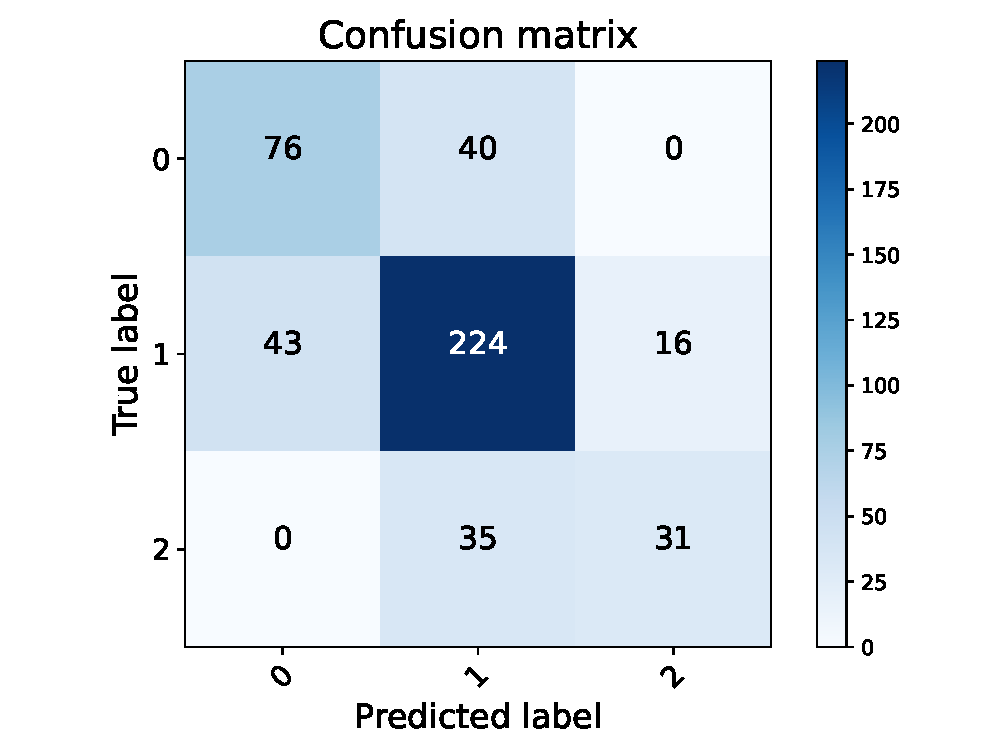
\includegraphics[width=0.6\textwidth]{files/figs/backg/conf-example.eps}
  \caption{An example of a confusion matrix. The entries on the diagonal are correctly classified, while the position of an off-diagonal entry shows what kind of error has been made. The true class is given by the row and the predicted class by the column.}
  \label{fig:conf-example}
\end{figure}

\section{Historical background of deep learning} \label{sec:dl-history}
In 1943, McCulloch and Pitts \cite{McCulloch1943} presented a mathematical model of a neuron which at the time had limited capabilities (e.g. it did not learn), but lay the foundations for much of what today is considered to be deep learning. Ivakhnenko and Lapa \cite{Ivakhnenko1965} introduced what would later be called deep learning with the first multi-layered network in 1965. The first convolutional network was introduced by Fukushima in 1980 \cite{Fukushima1980}.
A few years later, in 1989, LeCun et al. \cite{LeCun1989} showed it possible to train such networks with backpropagation and illustrated their effectiveness for computer vision problems. In 2009 Raina et al. \cite{Raina2009} suggested that \glspl{dnn} could efficiently be trained on \glspl{gpu}. Krizhevsky et al. \cite{Krizhevsky2012} used this when they with AlexNet proved it possible to train deeper networks which also greatly outperformed models of the time at computer vision tasks. Since then deep learning based methods has been adopted in various fields, such as computer vision, natural language processing, and even autonomous vehicles \cite{NazmusSaadat2020}.

\section{Deep Neural Networks}
\glspl{dnn} are combinations of linear and non-linear functions trained to approximate some other, potentially very complicated, function. The output of the network is formed as $f(x) = f_n \circ f_{n-1} \circ \hdots \circ f_1 \circ f_0(x)$ resulting in the layer terminology since the output from one function is passed as input to the subsequent one \cite{Goodfellow2016}.

Below the building blocks used in our work are briefly explained.

\subsubsection{Dense layer}
The dense, or fully connected, layer is the basic model for a feedforward network. The outputs of such a layer is formed as linear combinations of the inputs and bias terms. Usually a non-linear activation function is applied to this to be able to capture more general behaviors, resulting in the output

\begin{equation}
 y_i = h\Big( \sum_{j=1}^D w_{ij}x_j + b_i \Big)
 \label{eq:dense}
\end{equation}

where $h(\cdot)$ is a, possibly non-linear, activation function. $x_j$, $j \in \{1, \hdots, D\}$ are the inputs to the layer, $w_{ij}$ and $b_i$ are the weights and biases learned during training \cite{Bishop2006}. A network with two dense layers is shown in Figure \ref{fig:dense}.

\begin{figure}
 \centering
 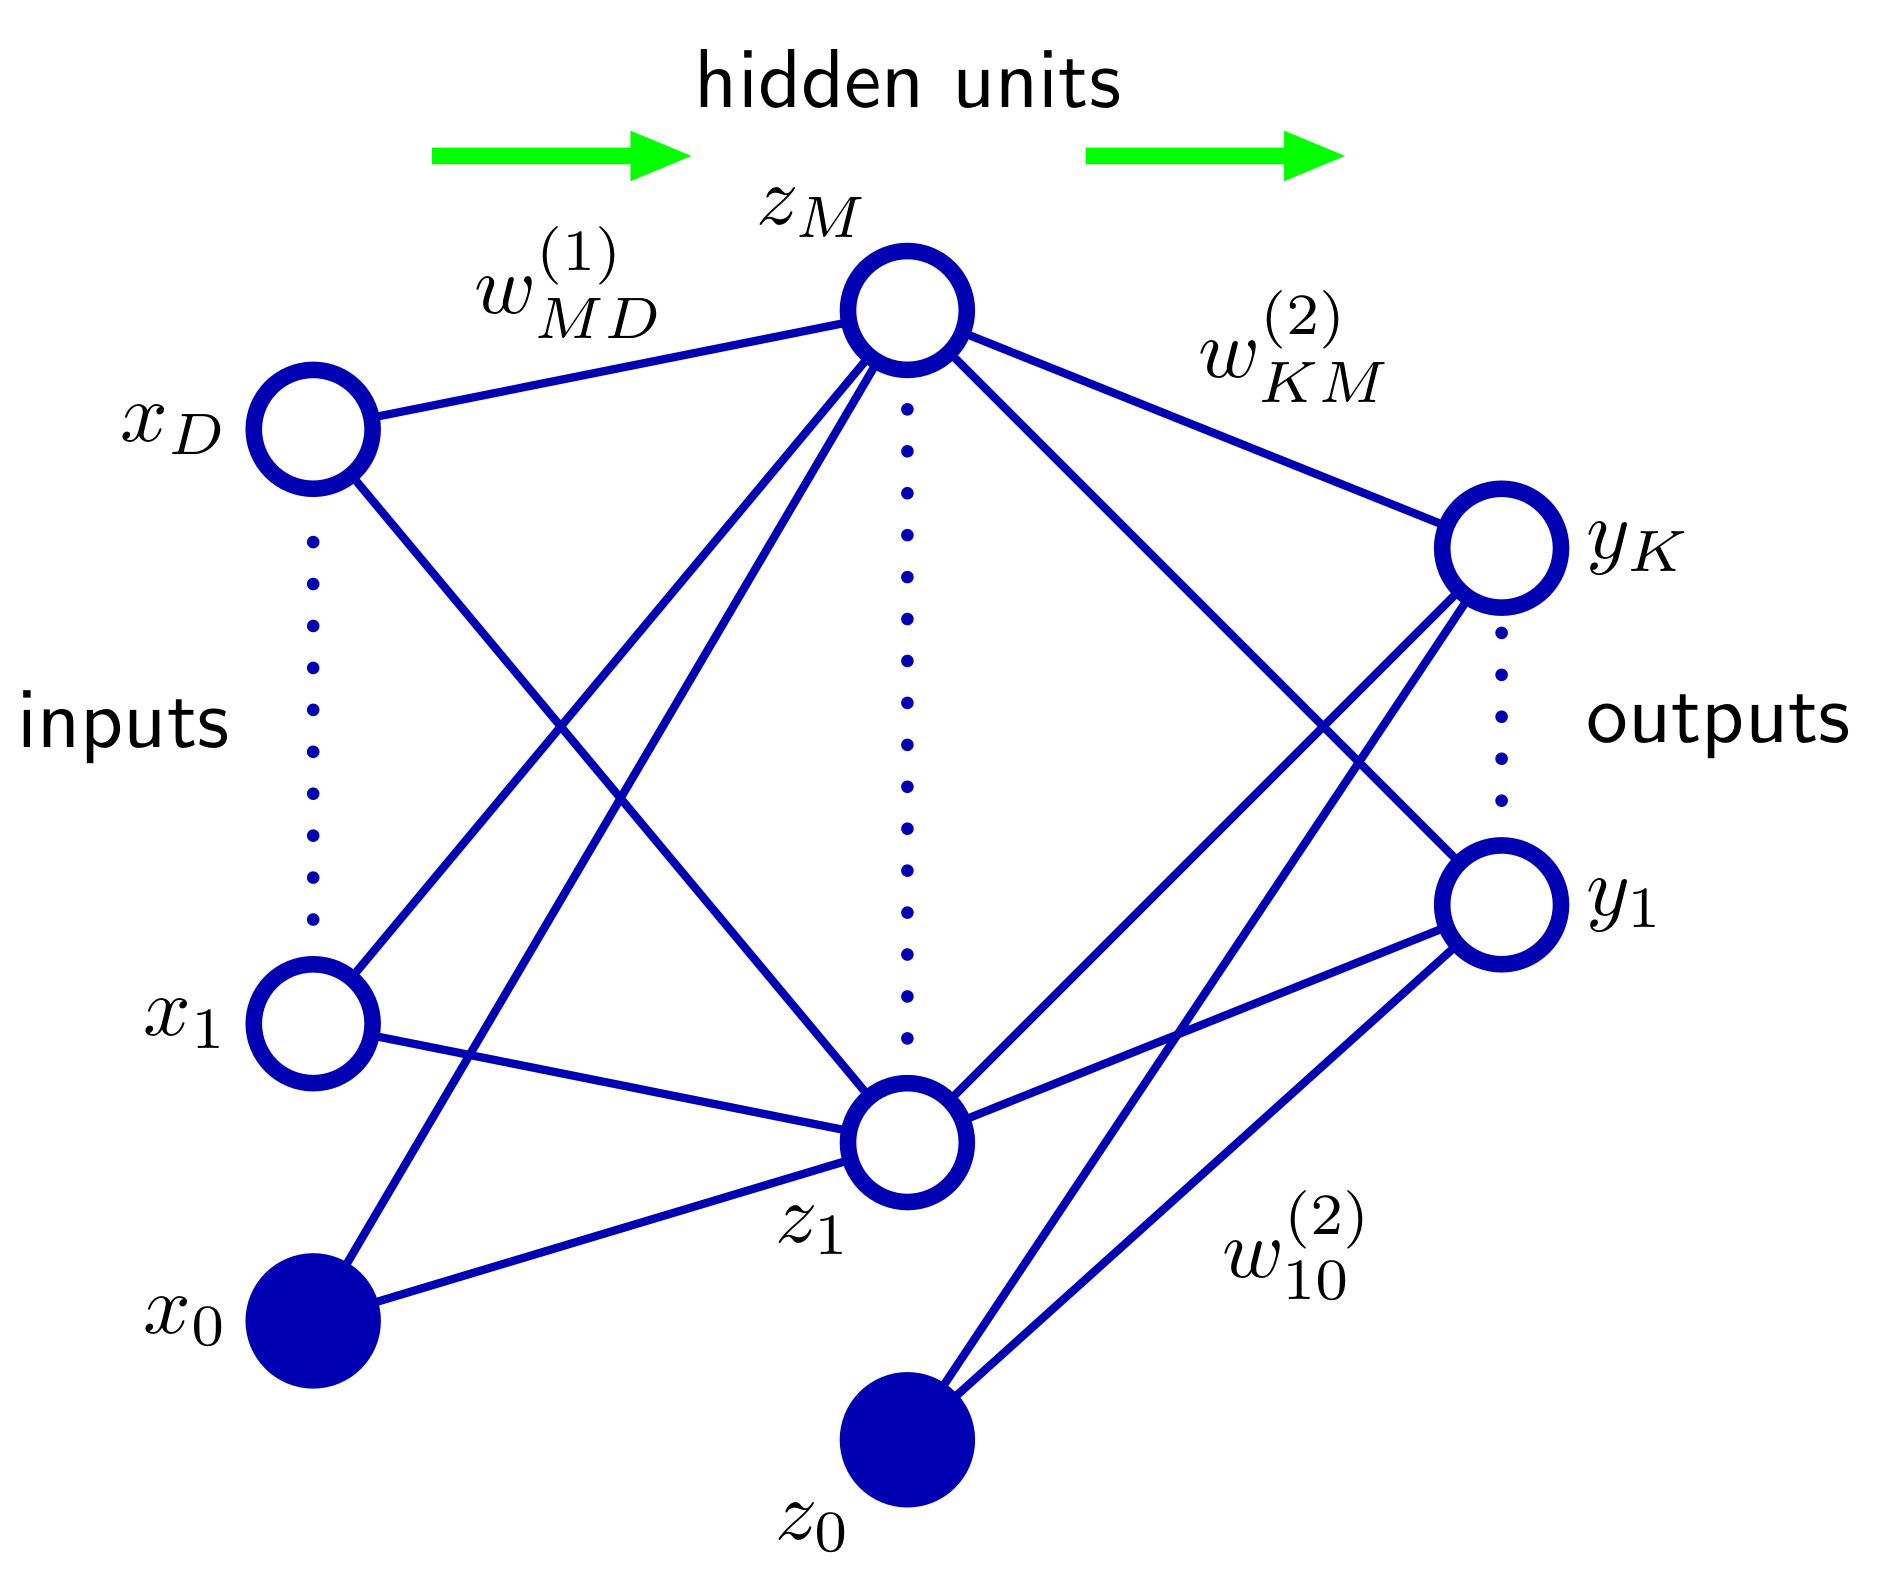
\includegraphics[width=0.5\textwidth]{files/figs/backg/mlp.png}
 \caption{Feedforward neural network with two densely connected layers. Each line corresponds to one trainable parameter. Here, $x_0$ and $z_0$ can be seen as ones added to the inputs introducing the bias terms \cite{Bishop2006}.}
 \label{fig:dense}
\end{figure}

% \FloatBarrier

\subsubsection{Convolutional layers}
Convolutional layers have proved successful for feature extraction from for instance time series or images. A reason for this is that they are equivariant to translation, meaning that patterns in a time series will be recognized in the same way no matter at which time steps they occur. The 1D convolution operation can be expressed as \eqref{eq:conv}.

\begin{equation}
 (x * w)(t) = \sum_{a=-\infty}^\infty x(a)w(t-a)
 \label{eq:conv}
\end{equation}

where $x$ is the input and $w$ is the kernel or filter which consist of the trainable parameters. As the kernel size is not affected by the input size the convolutional layer can be applied to inputs of different size, which is not possible with, for instance, the fully connected layer. When applied to images the convolution is performed in two dimensions. \cite{Goodfellow2016}.

% \FloatBarrier

\subsubsection{Pooling layers}
Pooling layers are used to reduce the dimensionality of feature maps. Common types of poolings are the max and the average pooling methods. Traditional max pooling represents nearby numbers by it maximum value while average pooling uses their average. This type of max pooling has proved efficient together with convolutional layers for computer vision tasks. Figure \ref{fig:pooling} illustrates how the pooling works. It can also be performed globally, i.e. on the entire feature map, which can be a way of handling differently sized data. For a \gls{tsc} problem, it is for instance possible to use size agnostic convolutional layers as feature extractors followed by a \gls{gap} layer resulting in a fixed size of the data to be classified \cite{Chollet2018}.

\begin{figure}
  \centering
  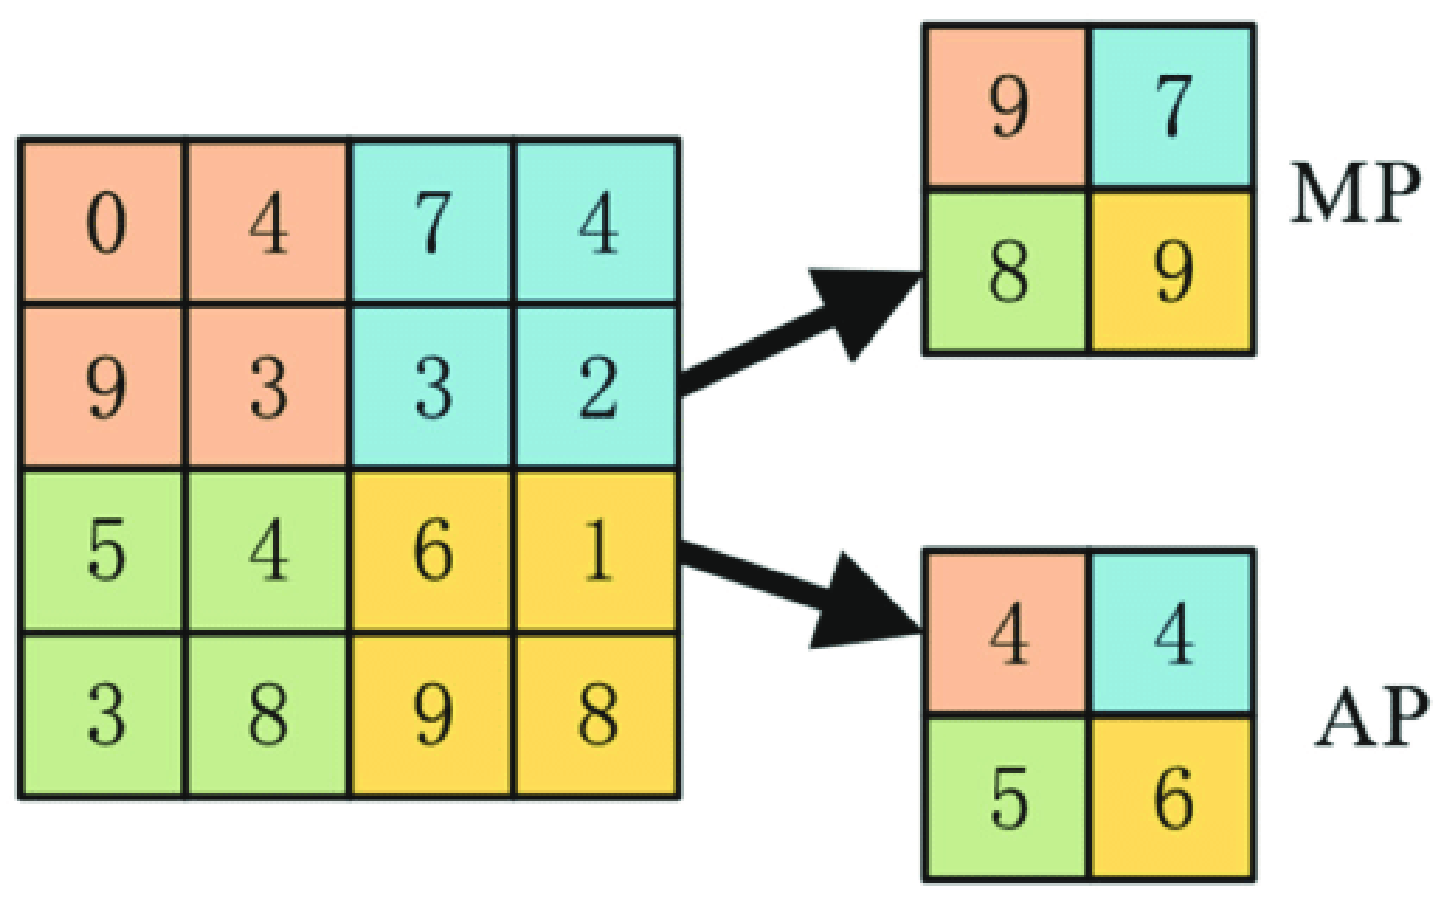
\includegraphics[width=0.4\textwidth]{files/figs/backg/pooling.png}
  \caption{Illustration of max and average pooling with pooling size 2$\times$2 and stride 2$\times$2. Image from \cite{Wang2018}.}
  \label{fig:pooling}
\end{figure}

% \FloatBarrier

\subsubsection{Activation functions}
The activation functions in a neural network has two main tasks. The first one is to introduce non-linearity to an otherwise linear model. The function $h(\cdot)$ in \eqref{eq:dense} is an example of such an activation function. A common such function is \gls{relu}, $h(z) = \max\{0,z\}$. Benefits with \gls{relu} is that it in its active region ($z>0$) does not have a suppressing effect on the gradient and it is easily computable. A drawback, however, is that the gradient is zero in its inactive region ($z < 0$) meaning gradient based training methods does not work here. An alternative to avoid this issue is the Leaky-\gls{relu} given by $h(z) = \max\{0.01 z, z\}$.
\gls{relu} and Leaky-\gls{relu} are shown in Figure \ref{fig:relu} and \ref{fig:leaky-relu}, respectively. Activation functions are also used for the output of the network, e.g. to obtain outputs representing probabilities. The sigmoid function, $h(z) = 1/(1+\exp(-z))$, shown in Figure \ref{fig:sigmoid}, can be used for this.
The sigmoid function will saturate the output between 0 and 1, however, if the model has several outputs e.g. representing the probabilities of the input belonging to different classes the total probability will not sum to 1. In this case the softmax function, $h(z)_i = \exp(z_i)/\sum_{j=1}^K \exp(z_j)$, can be used instead \cite{Goodfellow2016}. %With such an activation each output will be directly dependent on every other output .

\begin{figure}
  \centering
  \begin{subfigure}[t]{0.3\textwidth}
    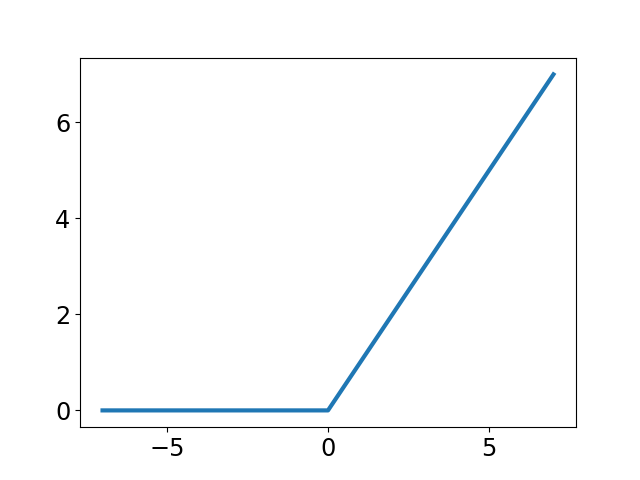
\includegraphics[width=\textwidth]{files/figs/backg/relu.png}
    \caption{ReLU}
    \label{fig:relu}
  \end{subfigure}
  ~
  \begin{subfigure}[t]{0.3\textwidth}
    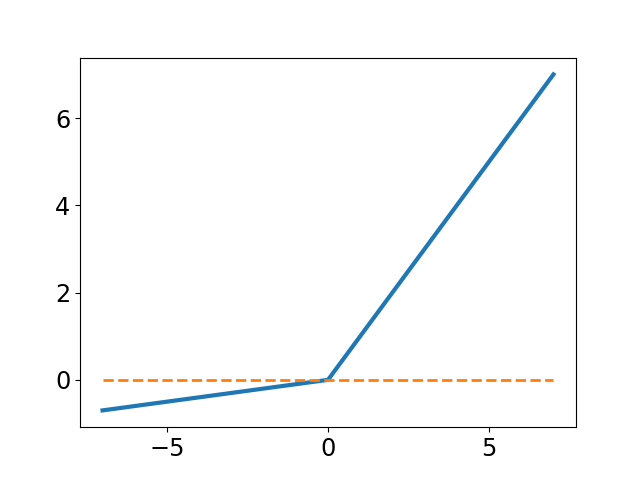
\includegraphics[width=\textwidth]{files/figs/backg/leaky_relu.png}
    \caption{Leaky-ReLU}
    \label{fig:leaky-relu}
  \end{subfigure}
  ~
  \begin{subfigure}[t]{0.3\textwidth}
    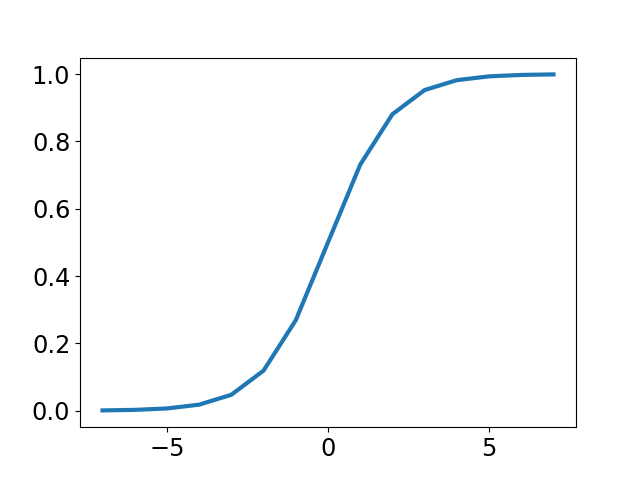
\includegraphics[width=\textwidth]{files/figs/backg/sigmoid.png}
    \caption{Sigmoid}
    \label{fig:sigmoid}
  \end{subfigure}
  \caption{Different activation functions, note that the slope of leaky ReLU for negative numbers is exaggerated for visualization purposes. }
  \label{fig:activations}
\end{figure}



\section{Training}
% The training of a network is performed by evaluating a loss function, which describes the desired behavior, on the training data.

During training of a network a loss function, $\mathcal{L}$, which describes the desired behavior, is evaluated on the training data. To improve the performance of the model its parameters are changed to minimize this loss. In deep learning problems, this optimization is usually performed with some gradient descent inspired method,

\begin{equation}
 \pmb{W}_{k+1} = \pmb{W}_k - \alpha \pmb{D},
 \label{eq:grad-desc}
\end{equation}

where $\pmb{W}_k$ denotes model parameters at iteration $k$, $\alpha$ the learning rate or step size, and $\pmb{D}$ the parameter update direction, e.g. $\frac{\partial \mathcal{L}}{\partial \pmb{W}}$ or a weighted average of earlier gradients.This means that the parameters are updated in the direction which reduces the loss the most. With a large training data set, the computation of the gradient quickly becomes expensive. A remedy for this has been to use stochastic or mini-batch gradient descent methods. Such algorithms use one or a few data points from the training set to estimate the gradient for each parameter update. Algorithms common today often use momentum, where previous gradients affect the parameter update direction, and adaptive learning rates (step size of parameter update), allowing different learning rate for different parameters \cite{Goodfellow2016}. One example of such a method is the Adam optimizer \cite{Kingma2015}.

The gradients of the loss with respect to the model parameters are calculated using the back-propagation algorithm \cite{Rumelhart1987} which recursively uses the chain rule,

\begin{equation}
 \frac{dz}{dx} = \frac{dz}{dy}\frac{dy}{dx},
 \label{eq:chain}
\end{equation}

to propagate the loss gradient through the network. For a network where $f_0, f_1, \hdots, f_n$ denotes the outputs of the $n+1$ layers, with corresponding layer parameters $\pmb{w}_0, \pmb{w}_1, \hdots, \pmb{w}_n$ and loss function $\mathcal{L}$, the gradient is calculated by first performing a forward pass of input $\pmb{x}$. This allows for computation of the the gradient w.r.t. the output of the final layer, $f_n$, either analytically or using automatic differentiation. As both the structure and the parameters of the layers are known this can be used to calculate the gradient w.r.t. the parameters in that layer, $\pmb{w}_n$, as well as the output of the previous layer, $f_{n-1}$. By applying

\begin{equation}
  \frac{\partial \mathcal{L}}{\partial f_k} & = \frac{\partial \mathcal{L}}{\partial f_{k+1}} \frac{\partial f_{k+1}}{\partial f_k} \label{eq:bp-layer}
\end{equation}

recursively, the gradient is propagated through the network and from this

\begin{equation}
  \frac{\partial \mathcal{L}}{\partial \pmb{w}_k} & = \frac{\partial \mathcal{L}}{\partial f_{k}} \frac{\partial f_{k}}{\partial \pmb{w}_k}
  \label{eq:bp-params}
\end{equation}

gives the gradients needed for the optimization.

% \begin{subequations} \label{eq:backprop}
%  \begin{align}
%   \frac{\partial \mathcal{L}}{\partial f_k} & = \frac{\partial \mathcal{L}}{\partial f_{k+1}} \frac{\partial f_{k+1}}{\partial f_k} \label{eq:bp-layer} \\
%   \frac{\partial \mathcal{L}}{\partial \pmb{w}_k} & = \frac{\partial \mathcal{L}}{\partial f_{k}} \frac{\partial f_{k}}{\partial \pmb{w}_k}    \label{eq:bp-params}
%  \end{align}
% \end{subequations}

\subsubsection{Loss functions}
For a classification problem with $K$ mutually exclusive classes the categorical cross-entropy is commonly used. With this loss the labels are one-hot encoded meaning that each label is represented by $K$ binary variables, i.e. $y_n \in \mathbb{Z}_2^K$. Each variable represents a class and $y_n^{(k)} = 1$ for the $k$ corresponding to the class of the label and 0 otherwise. The final layer of the model has $K$ outputs with softmax activation. The loss to be minimized is \cite{Bishop2006}

\begin{equation}
 \mathcal{L}(\pmb{x}, \pmb{W}) = - \sum_{n=1}^N \sum_{k=1}^K \lambda^{(k)} y_i^{(k)} \log \hat{y}_n^{(k)}(x_n, \pmb{W})
 \label{eq:cat-cross-entr}
\end{equation}
where $y_n^{(k)}$ denotes the correct binary label of class $k$ for data point $n$ in the training set, $\hat{y}_n^{(k)}$ the corresponding prediction from the model, and $\lambda^{(k)}$ weight for class.
% \begin{conditions}
%     $$y_n^{(k)}$$       & = & the correct binary label of class $k$ for data point $n$ in the training set \\
%     $$\hat{y}_n^{(k)}$$ & = & the corresponding prediction from the model \\
%     $$\lambda^{(k)}$$   & = & weight for class $k$.
% \end{conditions}

The categorical cross-entropy will aim to maximize the predicted probability for the correct class. However, incorrect probabilities have no direct effect on the loss. To be able to affect what kind of errors the model makes in its predictions a modification of this loss can be used. This modified loss, here referred to as confusion-entropy, introduces a matrix, $U$, which can be seen as a target confusion matrix distribution. Entries in $U$ rewards predictions at the corresponding positions in the confusion matrix, including possibly incorrect classifications. The confusion-entropy loss is \cite{Abbass2018}

\begin{equation}
    \mathcal{L}(\pmb{x}, \pmb{W}, U) = - \sum_{i=1}^K \sum_{j=1}^K u_{ij} \log \sum_{n=1}^N y_n^{(i)} \hat{y}_n^{(j)}(x_n, \pmb{W}).
    \label{eq:confusion-entropy}
\end{equation}


\section{Explainability} \label{sec:explainability}
Much of the recent progress in the deep learning space is inherently incomprehensible for us humans, due to its black-box nature and the size of the models \cite{Du2018}. However, explainability is important at many stages of the development of an AI-system. When the systems performance is at sub-human levels, it simplifies for human experts to improve it. When the system achieves similar results to those of human experts, it can help enforce trust to the system. Finally, in a scenario where the AI outperforms humans, it can help us get a better understanding of the problem \cite{Selvaraju2016}. With these methods playing a bigger role in fields such as healthcare the importance of explainable decisions also grows from a legal and ethical perspective \cite{Amann2020}.

\subsubsection{Gradient-weighted Class Activation Mapping (Grad-CAM)} \label{sec:grad-cam}
Although most deep learning models are not interpretable, there are post-hoc methods which tries to explain decisions. Selvaraju et al. \cite{Selvaraju2016} suggested one such method, called \gls{grad-cam}, where an activation map is calculated which shows what parts of the data is important for the decisions. This method is typically applied to the final convolutional layer ahead of, e.g., \gls{gap} layer. Let $y_c$ be the output corresponding to class $c$ and $A$ be the feature map, of height $H$, width $W$, and with $F$ filters, from which the activation should be calculated. The \gls{grad-cam} activation, $M_{GC}$, is then calculated as

% Considering a neural network with convolutional layers as feature extractors followed by \gls{gap} and dense layers for classification  is based on the final part of the network.

\begin{align}
 \begin{split}
  w_k^c &= \frac{1}{H \times W} \sum_{i=1}^H \sum_{j=1}^W \frac{\partial y_c}{\partial A_{ij}^k} \\
  M_{GC} &= ReLU \big ( \sum_{k=1}^F w_k^c A^k \big).
  \label{eq:grad-cam}
 \end{split}
\end{align}

With time series inputs, the resulting activation map, $M_{GC} \in \mathbb{R}^{H \times W}$, gives importance values for each time step if the network does not alter the time dimension of the data.% If the input is a time series this means that by designing the network to not alter the time dimension an importance value is obtained for each time step.

\section{Consistent Rank Logits (CORAL)}
Categorical data with a natural ordering are considered to be ordinal, examples of such data are the response to some medical treatment (e.g. poor, fair, good) \cite{Agresti2007} or the age of a person \cite{Cao2019}.

When classifying ordinal data, it is desirable to exploit the fact that the categories are ordered \cite{Agresti2007}. An ordinal classification problem, or ordinal regression as it is also referred to, can be formulated as assigning labels, $y \in \mathcal{Y} = \{\mathcal{C}_0, \mathcal{C}_1, \hdots, \mathcal{C}_{K-1} \}$, to inputs $\pmb{x}$, where the classes $\mathcal{C}_0 \prec \mathcal{C}_1 \prec \hdots \prec \mathcal{C}_{K-1}$ according to some ordering relation \cite{Cao2019}.

Li and Lin \cite{Li2007} presented a method for ordinal regression where the combined result of $K-1$ binary classifiers for $K$ classes were used. Each classifier checked whether the rank of the sample class was larger than rank $r_k \in \{r_1, \hdots r_{K-1}\}$. Niu et al. \cite{Niu2016} developed this further using a multi-output \gls{cnn} as $K-1$ binary classifiers, called OR-CNN. The classifiers share all weights except the ones in the output layer. This method achieved \gls{sota} performance on datasets where age was estimated based on facial images. However, consistency was not guaranteed in the predictions, e.g. sometimes simultaneously predicting an age under 20 and over 30.
Cao et al. \cite{Cao2019} addressed this issue with \gls{coral} which is an architecture-agnostic method that can extend any neural network based classifier. Similarly to OR-CNN \gls{coral} uses $K-1$ binary classifiers, here however sharing all weights parameters apart from the biases in the output layer. Instead of representing the labels as one-hot encodings they are now formed as $K-1$ binary labels, i.e. $y_n \in \mathbb{Z}_2^{K-1}$, where $y_n^{(k)} = 1$ if the rank of the class is greater than $r_k$ and 0 otherwise. The loss function to minimize is

\begin{equation}
 \mathcal{L}(\pmb{x}, \pmb{W}, \pmb{b}) = - \sum_{n=1}^N \sum_{k=1}^{K-1} \lambda^{(k)} [\log(\sigma(g(\pmb{x}_n, \pmb{W}) + b_k))y_n^{(k)} + \log(1 - \sigma(g(\pmb{x}_n, \pmb{W}) + b_k))(1 - y_n^{(k)})],
 \label{eq:coral-loss}
\end{equation}

where $\pmb{W}$ denotes all model parameters except biases of final layer, $\pmb{b}$ the bias weights of final layer, $\lambda^{(k)}$ the loss weight for rank $k$, $g(\pmb{x}_n, \pmb{W})$ the output of penultimate layer, $\sigma(z)$ the logistic sigmoid function, and $\sigma(g(\pmb{x}_n, \pmb{W}) + b_k)$ predicted output of the binary classifier.

% \begin{conditions}
%  $$\pmb{W}$$               & = & all model parameters except biases of final layer \\
%  $$\pmb{b}$$               & = & bias weights of final layer \\
%  $$\lambda^{(k)}$$         & = & loss weight for rank $k$ \\
%  $$g(\pmb{x}_n, \pmb{W})$$ & = & output of penultimate layer \\
%  $$\sigma(z)$$             & = & logistic sigmoid function, $1/(1 + \exp(-z))$ \\
%  $$\sigma(g(\pmb{x}_n, \pmb{W}) + b_k)$$ & = & predicted output of binary classifier $k$
% \end{conditions}

It can be shown that

\begin{equation}
 b_1 \geq b_2 \geq \hdots \geq b_{K-1}.
\end{equation}

The proof can be found in \cite{Cao2019} and from this and the shared weights it follows that

\begin{equation}
 \widehat{P} \big( y_n > r_1 \big) \geq \widehat{P} \big( y_n > r_2 \big) \geq \hdots \geq \widehat{P} \big( y_n > r_{K-1} \big)
\end{equation}

since the only thing that differs between the predictions is the bias. The probabilities for the individual classes are computed from this as

\begin{equation}
 \begin{alignedat}{2}
  &\widehat{P}\big(\mathcal{C}_0 \big) &&= 1 - \widehat{P}\big(y_n > r_1\big) \\
  &\widehat{P}\big(\mathcal{C}_1 \big) &&= \widehat{P}\big(y_n > r_1\big) - \widehat{P}\big(y_n > r_2\big) \\
  & &&\vdots \\
  &\widehat{P}\big(\mathcal{C}_{K-1} \big) &&= \widehat{P}\big(y_n > r_{K-1}\big).
 \end{alignedat}
\end{equation}

% !TEX root=../../mt-motion-analysis.tex
\chapter{Related work - Human Pose Estimation} \label{sec:pose_estimation} \label{ch:hpe}
\gls{hpe} is a well explored problem which, like many other computer vision tasks, has developed rapidly in recent years. The reasons behind this progress can mainly be explained by two factors. Firstly, the emergence of computing power discussed in Section \ref{sec:dl-history}, allowing for more expressive deep learning models. Secondly, several datasets with images labeled with human body joints has been made available \cite{Chen2020}. These datasets not only provide data, but also introduces competition in the research community, making it possible to compare the results of different approaches.

\section{Datasets} \label{sec:datasets}
%Some of the widely used datasets today are \gls{mpii} \cite{Andriluka2014}, \gls{coco} \cite{Lin2014}, \gls{aic-hkd} \cite{Wu2017}, and \gls{coco}-wholebody .% The two COCO datasets will now be described in more detail.

% In this work models trained on the \gls{coco} dataset are used. \gls{coco} consists of 328k images containing 91 different object types. The images come from Google, Bing, and Flickr image search and are mainly hand annotated through Amazon Mechanical Turk. The interesting part of the dataset for this work is the one with human poses. In total there are 250k instances of people labeled with joint locations \cite{Lin2014}. The joints, 17 per person, in the dataset can be seen in Figure \ref{fig:coco}. Along with the datasets containing body keypoints mentioned above there are also datasets with dense keypoints for specific bodyparts, e.g. OneHand10k \cite{Wang2019}. \gls{coco}-wholebody \cite{Jin2020} is an attempt to combine these two types of datasets by extending \gls{coco} with dense keypoints at hands, feet, and faces. The resulting 133 joints can be seen in Figure \ref{fig:coco-wholebody}.
In this work, models trained on the \gls{coco} dataset are used. \gls{coco} consists of 328k images containing 91 different object types. The images comes from Google, Bing, and Flickr image search and are mainly hand annotated through Amazon Mechanical Turk. The interesting part of the dataset for this work is the one with human poses. In total there are 250k instances of people labeled with joint locations \cite{Lin2014}. The joints, 17 per person, in the dataset can be seen in Figure \ref{fig:coco}. Along with the datasets containing body keypoints mentioned above there are also datasets with dense keypoints for specific bodyparts, such as hands or face. \gls{coco}-wholebody \cite{Jin2020} is an attempt to combine these two types of datasets by extending \gls{coco} with dense keypoints at hands, feet, and faces. The resulting 133 joints can be seen in Figure \ref{fig:coco-wholebody}.

\begin{figure}
 \centering
 \begin{subfigure}[t]{0.45\textwidth}
   \centering
  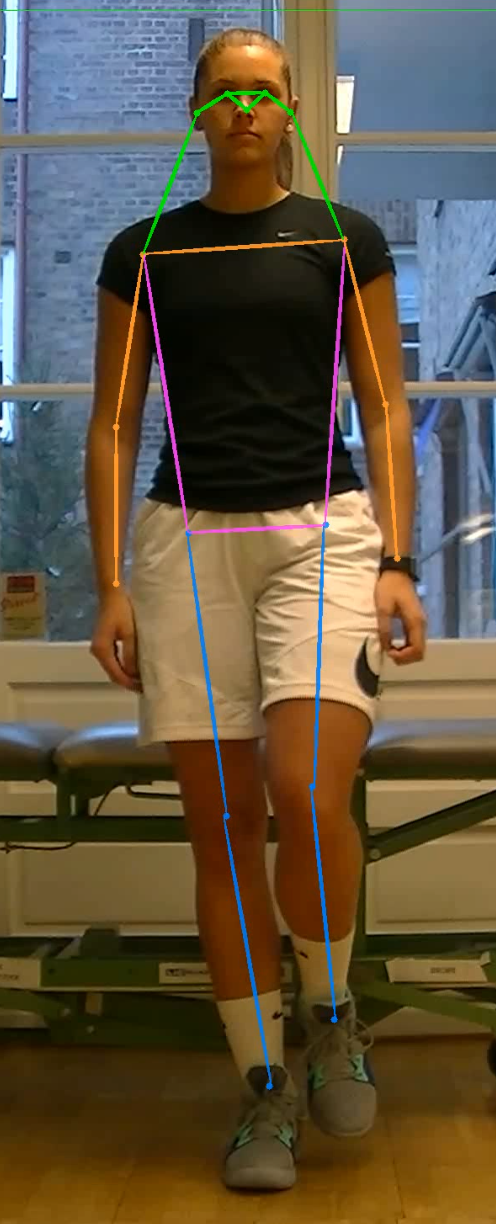
\includegraphics[width=0.6\textwidth]{files/figs/hpe/coco.png}
  \caption{Regular \gls{coco}.}
  \label{fig:coco}
 \end{subfigure}
 ~
 \begin{subfigure}[t]{0.45\textwidth}
   \centering
  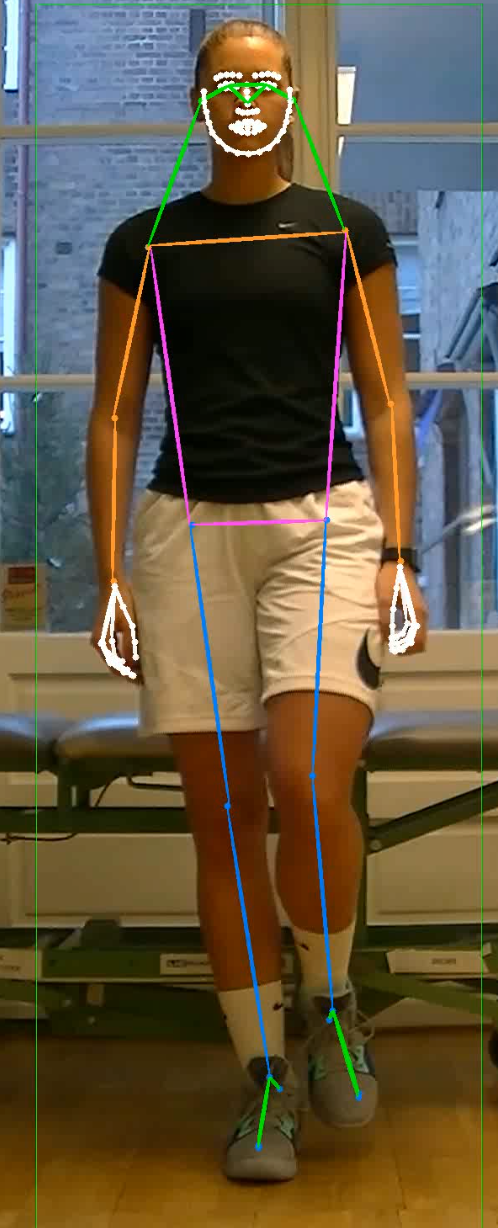
\includegraphics[width=0.6\textwidth]{files/figs/hpe/coco-wholebody.png}
  \caption{\gls{coco}-wholebody.}
  \label{fig:coco-wholebody}
 \end{subfigure}
 \caption{Keypoints for the two COCO datasets.}
\end{figure}

% \section{Pose estimation models}
\section{Background - Human pose estimation}
The \gls{hpe} problem has been explored since long before the most recent deep learning era. Pictoral Structures were introduced by Fishler and Elschlager in the 1970s. This meant identifying individual parts or features in images modeled with pair-wise spring-like connections \cite{Fischler1973}. After the progress of deep learning reviewed in Section \ref{sec:dl-history}, Toshev and Szegedy \cite{Toshev2014} presented DeepPose, the first \gls{hpe} method based on \glspl{dnn}, in 2014. Today's \gls{hpe} methods are generally categorized as top-down or bottom-up approaches. This has to do with how they handle multiple persons. Bottom-up models starts by finding all keypoints for all persons in an image and then match them together to form persons. Top-down models on the other hand starts by finding bounding boxes for all individuals and then identifies keypoints for one person at a time. The sequential nature of the top-down methods and the fact that two models are needed means that bottom-up models scale better with the number of persons to analyze. However, top-down models tends to be more accurate \cite{Cheng2019}.
% Since the application we present requires single person recognition only the top-down \gls{sota} methods presented below are used.

\section{Pose estimation models}
Below the \gls{hpe} models used in our work are presented. As we are interested in single person recognition, the model used is of top-down type.

\subsection{High-Resolution Net (HRNet)} \label{sec:hrnet}
Sun et al. presented the \gls{hrnet} \cite{Sun2019} architecture in 2019, initially for \gls{hpe}, but also for other computer vision tasks such as semantic segmentation and object detection. Such problems had traditionally been solved using networks built on high-to-low resolution convolutions with increasing numbers of feature maps (e.g ResNet \cite{He2016}, VGGNet \cite{Simonyan2015}). The classification task was solved in the low-resolution space and then transformed back to form the high-resolution representation needed for e.g. the \gls{hpe}. Sun et al's proposed architecture preserves a high resolution representation throughout the network. It does so while also producing low-resolution/high dimensional representations suitable for classification.

The network architecture is shown in Figure \ref{fig:hrnet} and consists of four stages (blue blocks in depth direction in the figure) with convolutional layers. After each stage a new low-resolution representation is created by performing strided convolutions. At these instances, the existing representations also exchange information by either nearest neighbor upsampling or strided convolutions. The $K$ estimated keypoints are represented as heatmaps, $\{\mathbf{H}_1, \hdots, \mathbf{H}_K\}$, indicating the locations. These heatmaps are formed from the last high-resolution feature map (top right in Figure \ref{fig:hrnet}). Corresponding ground truth heatmaps are generated by applying 2D Gaussians to the correct keypoint locations and the model is trained by minimizing the mean squared error between these \cite{Sun2019}. Although a high resolution heatmap is desirable as it gives smaller quantization errors, the computational cost increases quadratically with the size \cite{Zhang2020}. Hence, the performance of the model can be improved by extracting the region of interest from the input image. This can for instance be done using an object detection model trained to find humans.

Object detectors usually work by first producing a large number of regions of interest in the image which are then classified to either belong to some object class or the background. Faster R-CNN by Ren et al. \cite{Ren2017} is an example of such a detector where these steps are performed by a single \gls{cnn}. The model outputs bounding boxes and class scores for the objects in the image deemed not to be part of the background.

\begin{figure}
 \centering
 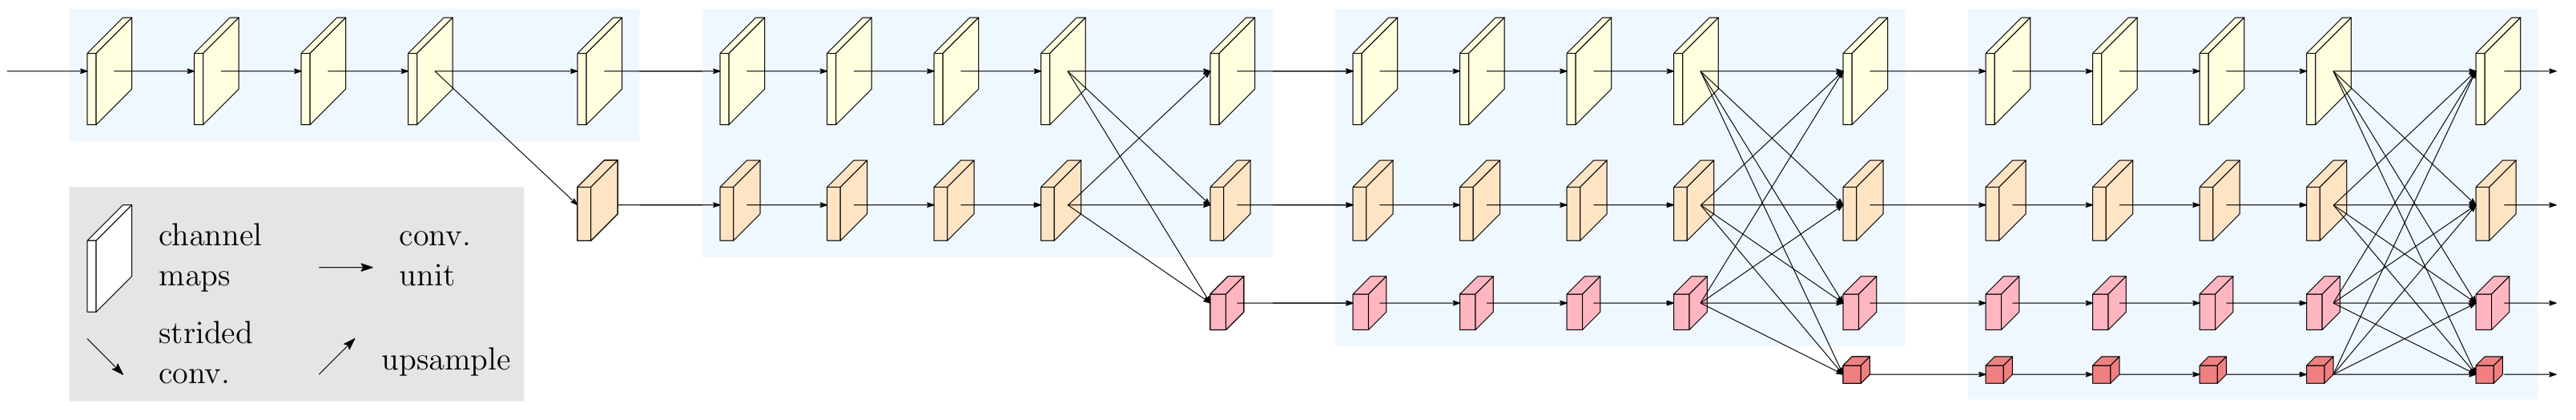
\includegraphics[width=\textwidth]{files/figs/hpe/hrnet.png}
 \caption{Network architecture for HRNet. The top row shows high resolution representations with fewer number of feature maps. Each step downwards reduces the resolution with a factor of two while the number of feature maps are doubled \cite{Wang2020}.}
 \label{fig:hrnet}
\end{figure}

% \FloatBarrier

\subsection{Distribution-Aware coordinate Representation of Key-point (DARK)} \label{sec:dark}
As discussed above a high resolution heatmap should result in higher accuracy, but is computationally expensive. Zhang et al. propose a method they call \gls{dark} \cite{Zhang2020} to reduce the quantization error by i) analyzing the distributions of the predicted heatmaps, and ii) creating the training heatmaps in a slightly new fashion.

The actual keypoint location is found at the maximal activation of the heatmap. Since it is smaller than the actual image this turns into a sub-pixel localisation problem. Newel et al. \cite{Newell2016} empirically found that good results may be found using a weighted average between the two highest activations,

\begin{equation}
  \pmb{p} = \symbfit{m} + \frac{1}{4}\frac{\symbfit{s} - \symbfit{m}}{\lVert \symbfit{s} - \symbfit{m} \rVert_2},
  \label{eq:pixel-empiric}
\end{equation}
where \italbf{p} denotes the predicted maximum, \italbf{m} the highest activation, and \italbf{s} the second highest activation.
% \begin{conditions}
%        & =   & predicted maximum \\
%     \italbf{m}      & =   & highest activation \\
%     \italbf{s}      & =   & second highest activation
% \end{conditions}

This has been the de facto standard heatmap decoding, but Zhang et al. suggests using the fact that the heatmaps used for training usually are created as 2D Gaussian distributions, i.e. that the heatmaps can be expressed as

\begin{equation}
  \mathcal{G}(\pmb{x}; \pmb{\mu}, \Sigma) = \frac{1}{2\pi \mid \Sigma \mid^{\frac{1}{2}}}
  \exp \Big( -\frac{1}{2} (\pmb{x} - \pmb{\mu})^\intercal \Sigma^{-1} (\pmb{x} - \pmb{\mu}) \Big)
  \label{eq:gaussian-heatmap}
\end{equation}

where $\pmb{\mu}$ denotes the maximum of the heatmap, \italbf{x} the pixel location, and $\Sigma$ a diagonal covariance matrix.

By Taylor expanding the logarithm of \eqref{eq:gaussian-heatmap} in the point \italbf{m}, i.e. the point with the highest sampled activation, an expression for $\pmb{\mu}}$ is obtained as

\begin{equation}
    \pmb{\mu} = \pmb{m} - \Big(\mathcal{D''}(\pmb{m})\Big)^{-1} \mathcal{D'}(\pmb{m})
    \label{eq:opt-mu}
\end{equation}
where $\mathcal{D}(\pmb{x}) = -\frac{1}{2} (\pmb{x} - \pmb{\mu})^\intercal \Sigma^{-1} (\pmb{x} - \pmb{\mu})$, i.e., the non constant term in the logarithm of $\mathcal{G}$ in \eqref{eq:gaussian-heatmap}.
% \begin{conditions}
%     $$\mathcal{D}(\pmb{x})$$ & = & $-\frac{1}{2} (\pmb{x} - \pmb{\mu})^\intercal \Sigma^{-1} (\pmb{x} - \pmb{\mu})$, \\
%       & & i.e. the non constant term in the logarithm of $$\mathcal{G}$$
% \end{conditions}

The derivatives $\mathcal{D'}(\pmb{m})$ and $\mathcal{D''}(\pmb{m})$ are efficiently estimated from the heatmap. As this approach strongly assumes a Gaussian structure, it is proposed to modulate the heatmap before estimating the maximal activation. This is done by performing a convolution with a Gaussian kernel with the same covariance as the one used for the training data.

\begin{figure}[H]
  \centering
  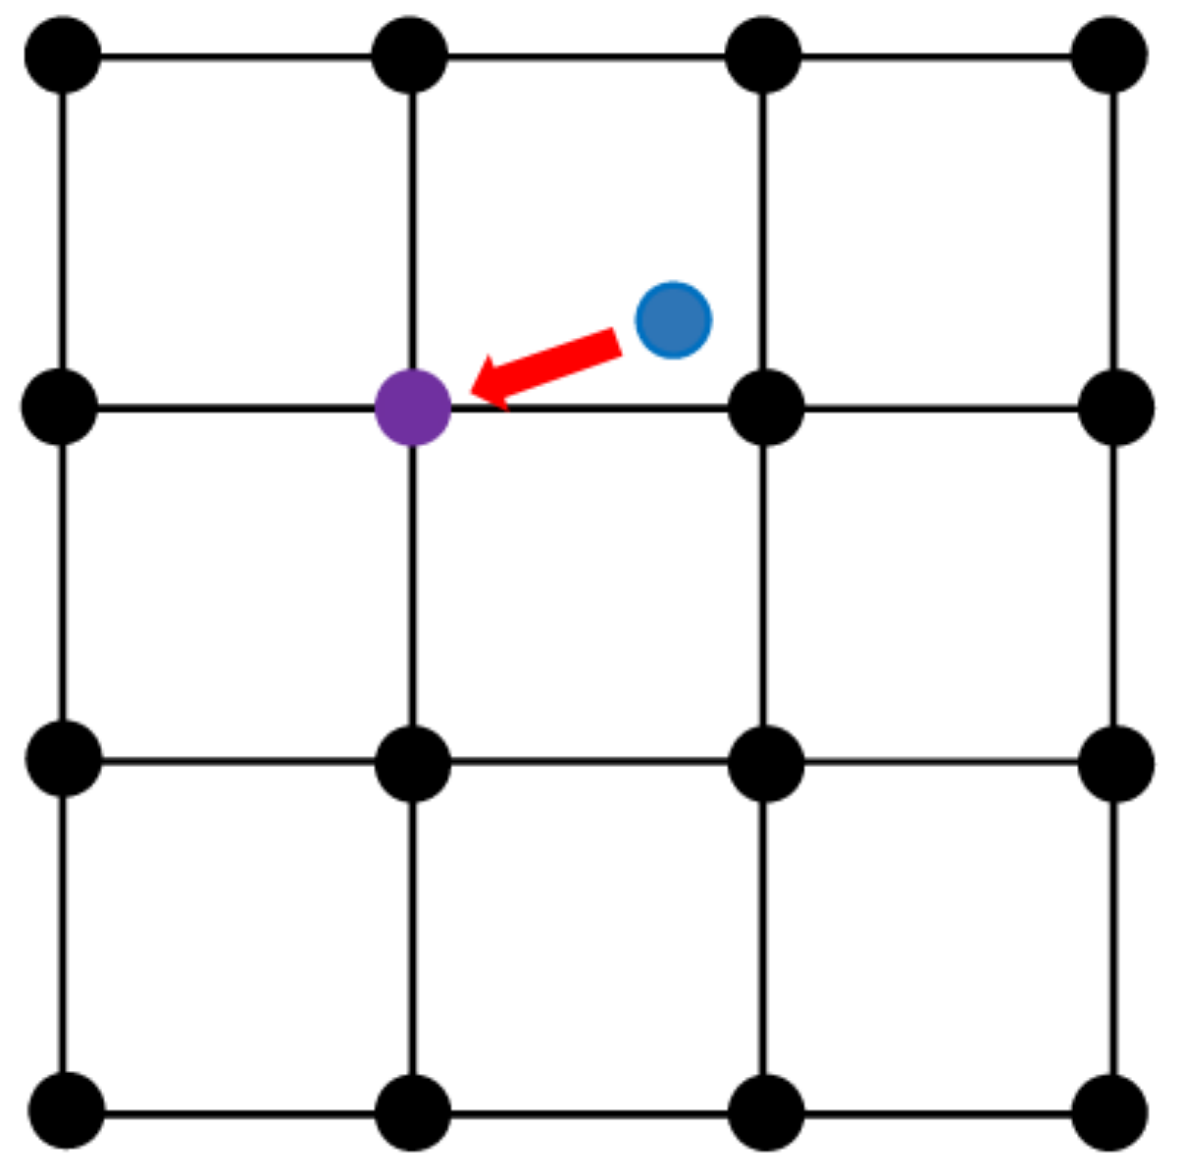
\includegraphics[width=0.4\textwidth]{files/figs/hpe/quantization.png}
  \caption{Quantization error due to off-grid keypoint location. Correct location (blue) represented by on-grid coordinate \cite{Zhang2020}.}
  \label{fig:pixel-quantization}
\end{figure}

The second improvement suggested by Zhang et al. concerns the creation of the training heatmaps. Traditionally, these have been created from the quantized keypoint locations, resulting in a slightly biased heatmap. In Figure \ref{fig:pixel-quantization}, this would correspond to having the peak activation in e.g. the purple dot. By instead using the non-quantized location, an unbiased heatmap is obtained. This would correspond to having the peak off-grid, in the blue dot in Figure \ref{fig:pixel-quantization}. Combining this with the method described above using derivatives to predict the location of the maximum seems to improve the accuracy of pose estimators.

The \gls{dark} method is model agnostic and can be used with any pose estimator as it is just a slightly different way of generating the training heatmaps and analyzing the output heatmaps.

% \FloatBarrier

% The combination of DARK and HRNet is the method that as of today yields the highest accuracy on both the COCO and MPII dataset

% !TEX root=../../mt-motion-analysis.tex
\chapter{Related work - Time Series Classification} \label{sec:tsc} \label{ch:tsc}
\section{Background - Time series classification}
Time series are sequences of data ordered in some dimension, e.g. time. They can be univariate, i.e. containing one variable, or multivariate and they can be used to describe any ordered, discrete data, for instance information extracted from videos.

\begin{definition}
  \text{A univariate time series of length n, with ordered indices}
  $$X = \left[x_1, x_2, \hdots, x_n\right]^\intercal$$
  \label{def:uts}
\end{definition}

\begin{definition}
    \text{A multivariate time series of length n, with M channels}
    $$\pmb{X} = \left[X_1, \hdots, X_M\right]$$
\end{definition}

The \gls{tsc} task is about finding a function, $f: \mathbb{R}^{n \times M} \rightarrow \mathbb{R}$, that assigns one label to each, possibly multivariate, time series. The problem bears strong resemblance with that of image classification, but with the two spatial dimensions replaced by one temporal dimension. Despite this the use of end-to-end deep learning models is not as dominant in the \gls{tsc} community \cite{IsmailFawaz2019}. Instead it is common to manually extract features deemed suitable for classification. Similarily to the fields of computer vision various datasets has emerged recently. This has been important for the development of \gls{tsc} as it allows for fair comparison between methods. One of the most widely used dataset collections today is the \gls{ucr} archive \cite{Dau2018} containing 85 different time series datasets.

Traditionally a nearest neighbor method together with dynamic time warping has been common for classification \cite{Bagnall2017}. Simply put, this means that a time series during classification is compared to the training data and assigned the class of the most similar time series. Lines and Bagnall suggested a method where an ensemble of 11 nearest neighbor classifiers with different similarity measures \cite{Lines2015} which yielded \gls{sota} results. Bagnall et al. \cite{Bagnall2015} developed the idea of ensemble based classifiers with \gls{cote}, where 35 different classifiers using different transforms were used.
Lines et al. \cite{Lines2016} extended \gls{cote} further with two new classifiers resulting in \gls{hive-cote}. One drawback with \gls{hive-cote} is the computational intensity, both during training and test time. Training time is large partly due to one of the transforms used is the Shapelet Transform with a time complexity of $O(n^2l^4)$, $n$ being the number of time series and $l$ the length of them. Due to the nature of the nearest neighbor algorithm, the result of the 37 classifiers during test time needs to be compared to the corresponding result for each time series in the training set, causing this method to be impractical for real-time use \cite{IsmailFawaz2019}.

In 2016 Zheng et al. \cite{Zheng2016} presented a neural network model based on convolutional layers for the classification task. Wang et al. \cite{Wang2017} developed these ideas and presented models with performance close to that of \gls{cote} on the \gls{ucr} archive. The development of neural network based classification has since then continued and below two architectures which are either used or have inspired our work are presented.

\section{Deep learning architectures}
The last few years the number of proposed neural network based time series classifiers has increased drastically. Below the two most influential architectures for our work are presented.

\subsection{InceptionTime} \label{sec:inception-time}
InceptionTime, presented by Fawaz et al. \cite{IsmailFawaz2020}, is, as the name suggests, inspired by Inception \cite{Szegedy2015} which is an architecture successful in computer vision tasks. It is comprised of several stacked Inception modules consisting of differently sized convolutions as well as pooling layers. To reduce the number of parameters in the network 1$\times$1 convolutions are often used as a dimensionality reduction.
One such module can be seen in Figure \ref{fig:inception-module}. The architecture of Fawaz et al. is similar, but with only one temporal dimension instead of two spatial dimensions. The number of filters in the convolutions and the length of these filters are hyperparameters to be tuned. All convolutions use the same number of filters to simplify the tuning and the same length parameter is also used throughout the network. The length of the three parallel filters is given by $0.5^k* \text{filter\_length}$, $k = [0,1,2]$. Thus the length parameter in Figure \ref{fig:inception-module} is 40. As with the computer vision task the dimensionality is reduced, here through a bottleneck of size $m$. The bottleneck is achieved by convolutions with $m$ filters of length 1. The InceptionTime module is shown in Figure \ref{fig:inceptiontime-module}.

Figure \ref{fig:inceptiontime} shows how stacked modules makes up the InceptionTime architecture. Residual connections are used to decrease the risk of vanishing gradients once the network becomes deeper, as suggested by He et al. \cite{He2016}. The InceptionTime modules are followed by a \gls{gap} layer which averages each time series over its time dimension. The classification is performed by fully connected layers with softmax activations.

Many deep learning based time series classifiers experiences a significant variance in their accuracy, especially when evaluated on the \gls{ucr} archive with rather small training sets \cite{IsmailFawaz2019ensemble}. To overcome this Fawaz et al. suggest the use of an ensemble of identical InceptionTime networks, but with randomly initialized weights before training. The ensemble's output is then calculated as the average of the outputs of the individual models. Such an ensemble of five models achieves a performance similar to that of \gls{hive-cote} on the \gls{ucr} archive.
% As was showed with ResNet \cite{He2016} residual connections reduces the risk for vanishing gradients and enables deeper networks. Hence this is

% Using residual connections between blocks reduces the risk of vanishing gradients and allows for deeper networks

%The 1D convolutions together with dimensionality reduction allows for longer filters than what is feasible to use for images.

\begin{figure}
  \centering
  \begin{subfigure}[c]{0.6\textwidth}
    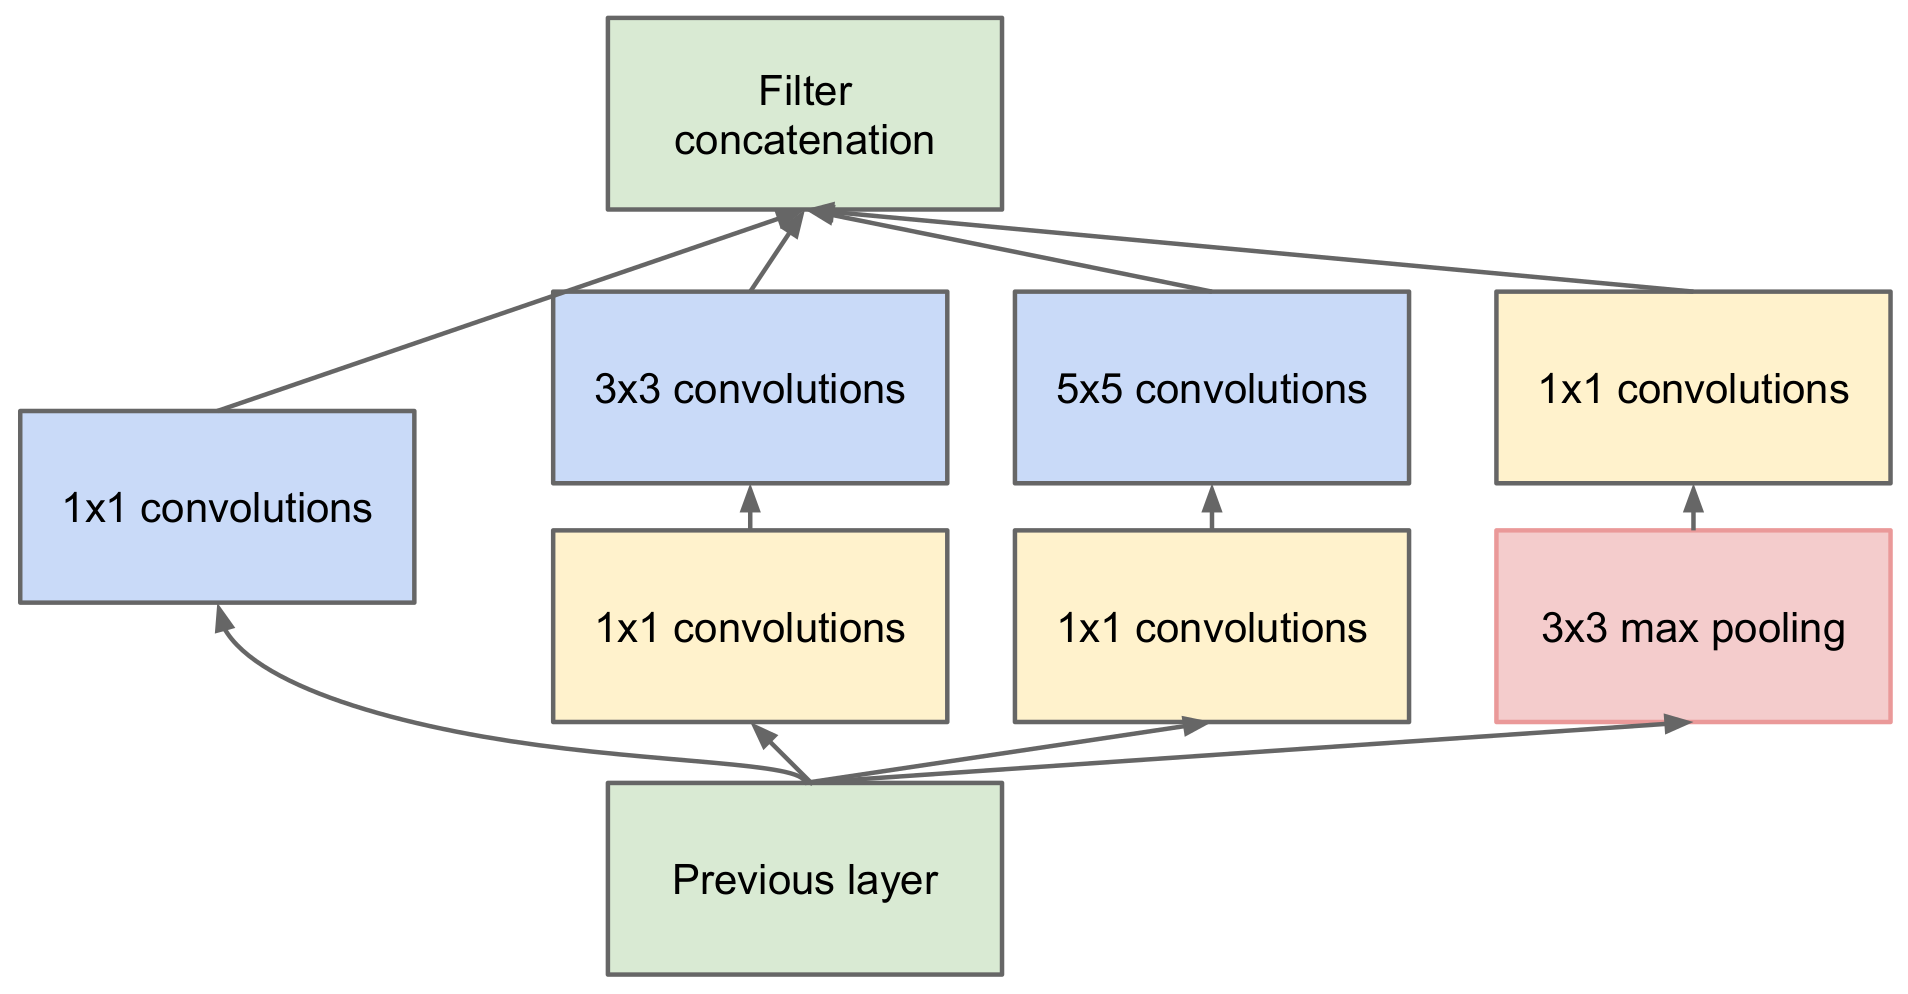
\includegraphics[width=\textwidth]{files/figs/tsc/inception-module-dimred.png}
    \caption{}
    % \caption{Inception module for computer vision \cite{Szegedy2015}.}
    \label{fig:inception-module}
  \end{subfigure}
  \begin{subfigure}[c]{0.6\textwidth}
    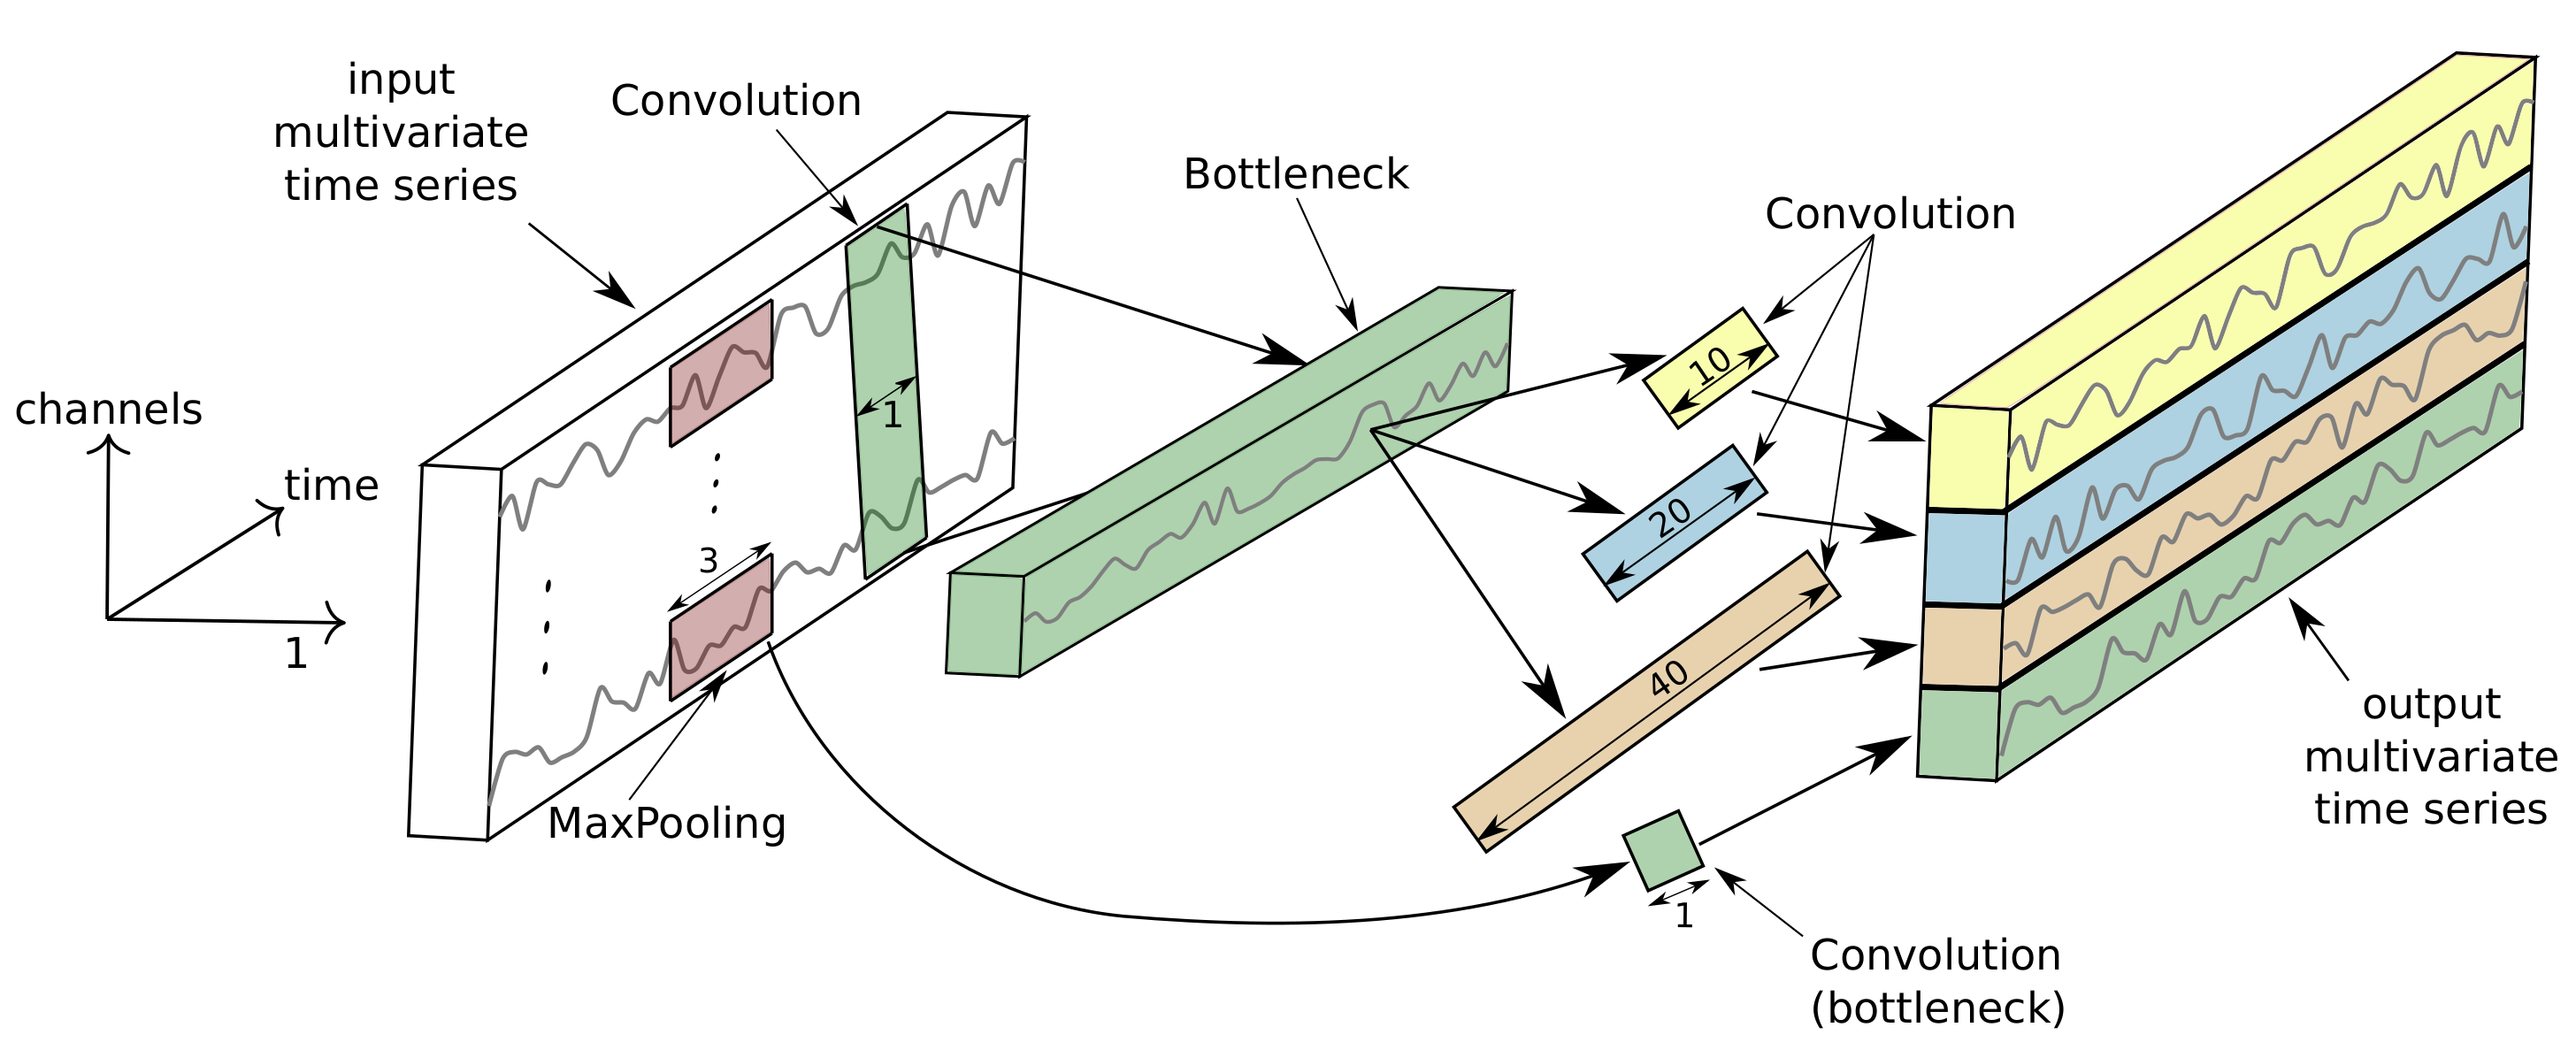
\includegraphics[width=\textwidth]{files/figs/tsc/inception-time-module.png}
    \caption{}
    % \caption{Inception module for \gls{tsc} \cite{IsmailFawaz2020}.}
    \label{fig:inceptiontime-module}
  \end{subfigure}
  \caption{Inception modules for computer vision (a) with dimensionality reduction ahead of the 3$\times$3 and 5$\times$5 convolutions and InceptionTime module for TSC (b), here illustrated with a bottleneck size of 1. Figures from \cite{Szegedy2015} and \cite{IsmailFawaz2020} respectively.}
\end{figure}

\begin{figure}
  \centering
  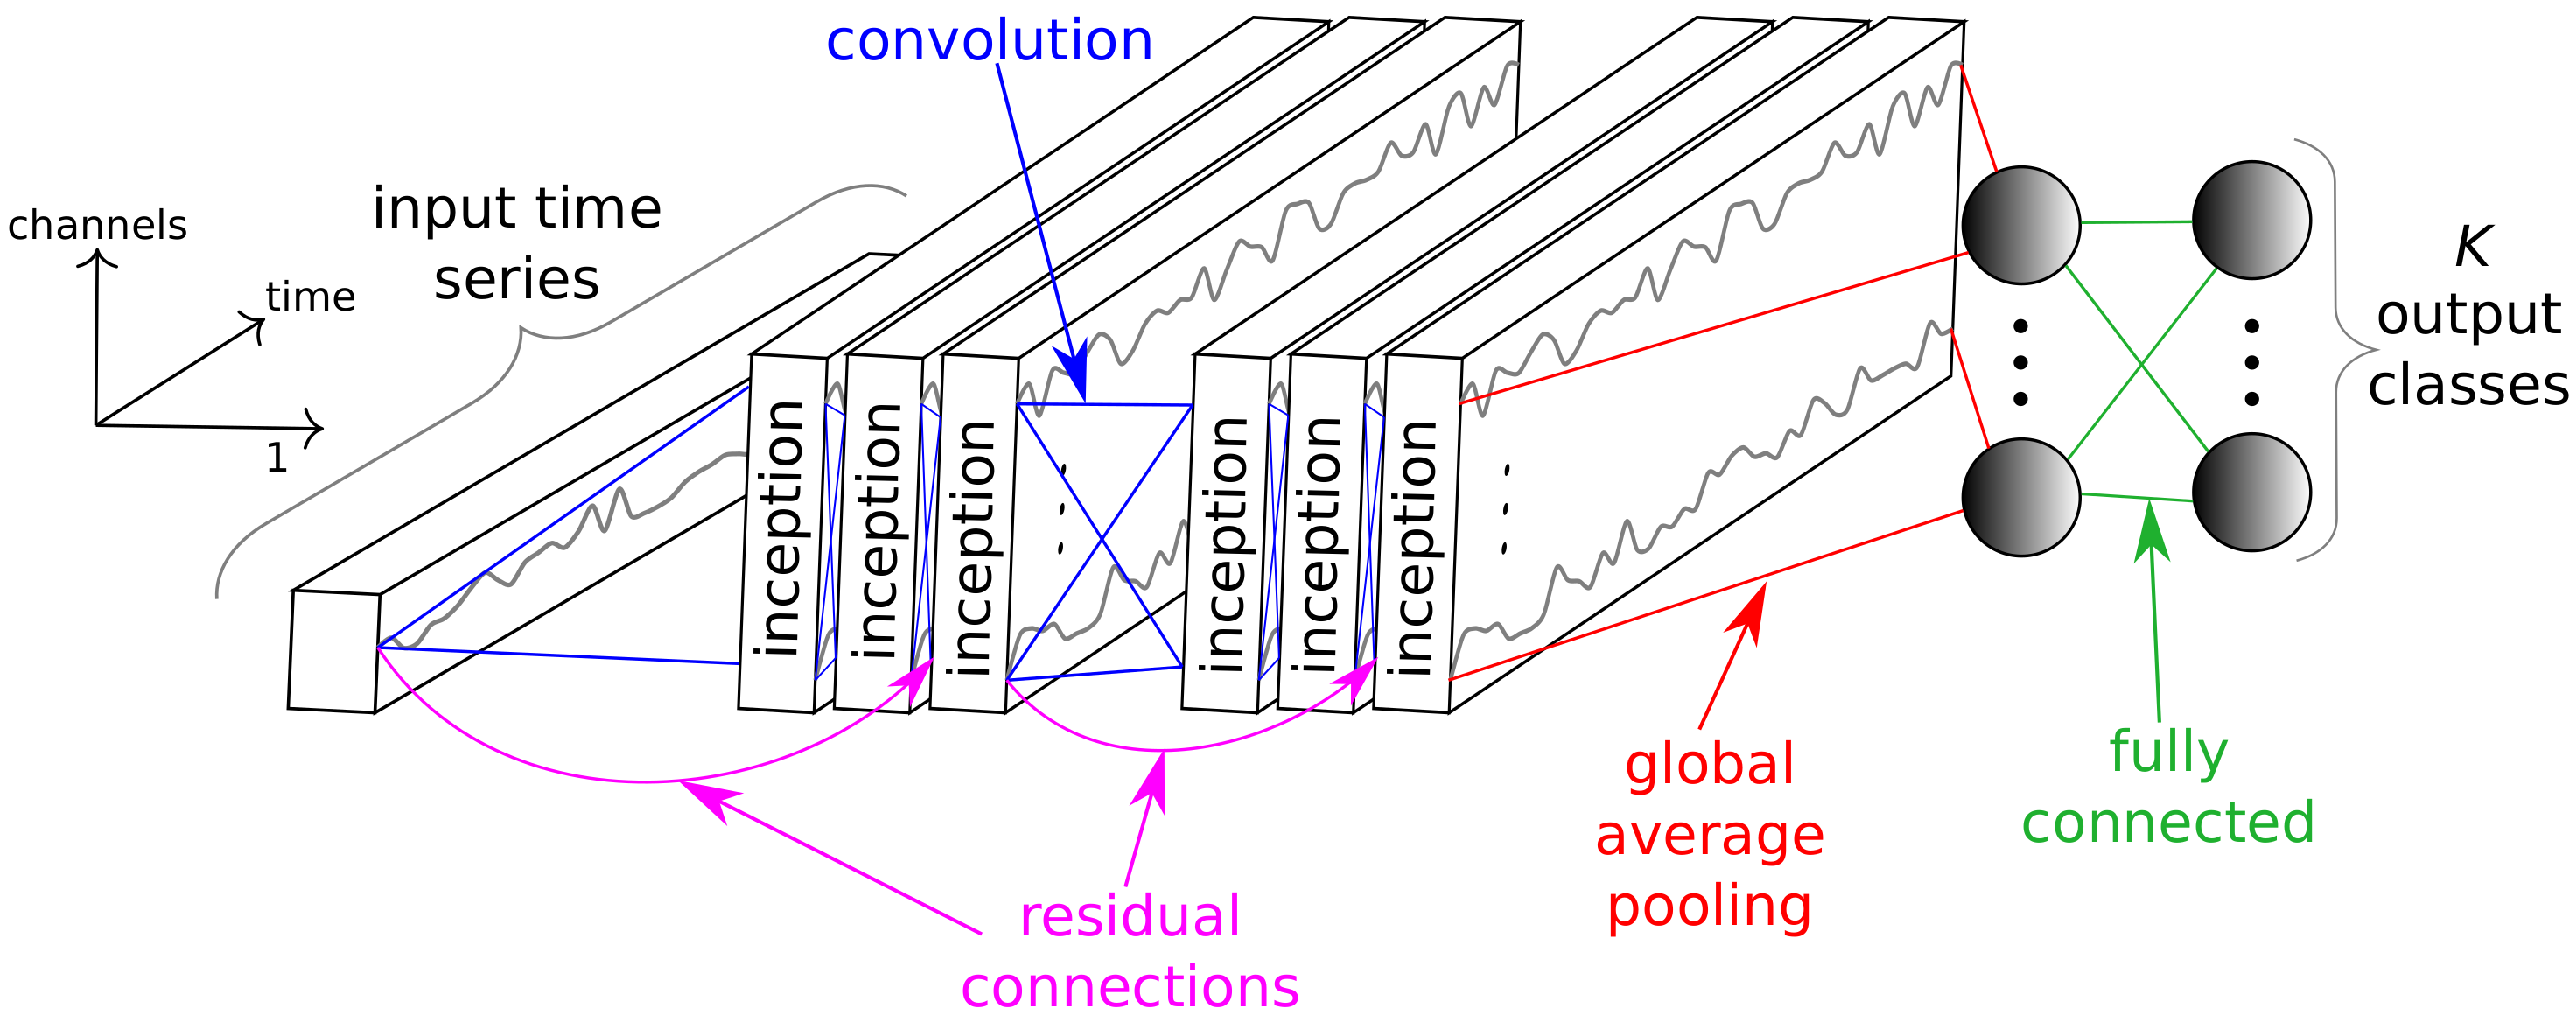
\includegraphics[width=0.6\textwidth]{files/figs/tsc/inceptiontime.png}
  \caption{InceptionTime architecture for TSC \cite{IsmailFawaz2020}.}
  \label{fig:inceptiontime}
\end{figure}

% \FloatBarrier

\subsection{Explainable Convolutional Neural Network for Multivariate Time Series Classification (XCM)} \label{sec:XCM}
As discussed in Section \ref{sec:explainability} explainability is desirable, but not inherent in most black-box deep learning models. Fauvel et al. \cite{Fauvel2020} propose an architecture, \gls{xcm}, which allows for tracking which time steps and which inputs are important for the classification decision. By using 2D convolutions with kernels of size $ks$$\times$1, where $ks$ is the kernel size hyperparameter, the convolution is only performed in the time dimension and the input channels are kept separated throughout the feature extraction.
Through dimensionality reduction from a 1$\times$1 2D convolution a single feature map for each input is produced. From this, the importance of input channels and time steps can be traced using \gls{grad-cam}, described in Section \ref{sec:grad-cam}. In parallel to the channel specific features Fauvel et al. also suggests using 1D convolutions over all channels resulting in a combined feature map along the time dimension. The \gls{xcm} architecture is depicted in Figure \ref{fig:xcm}.

\begin{figure}
  \centering
  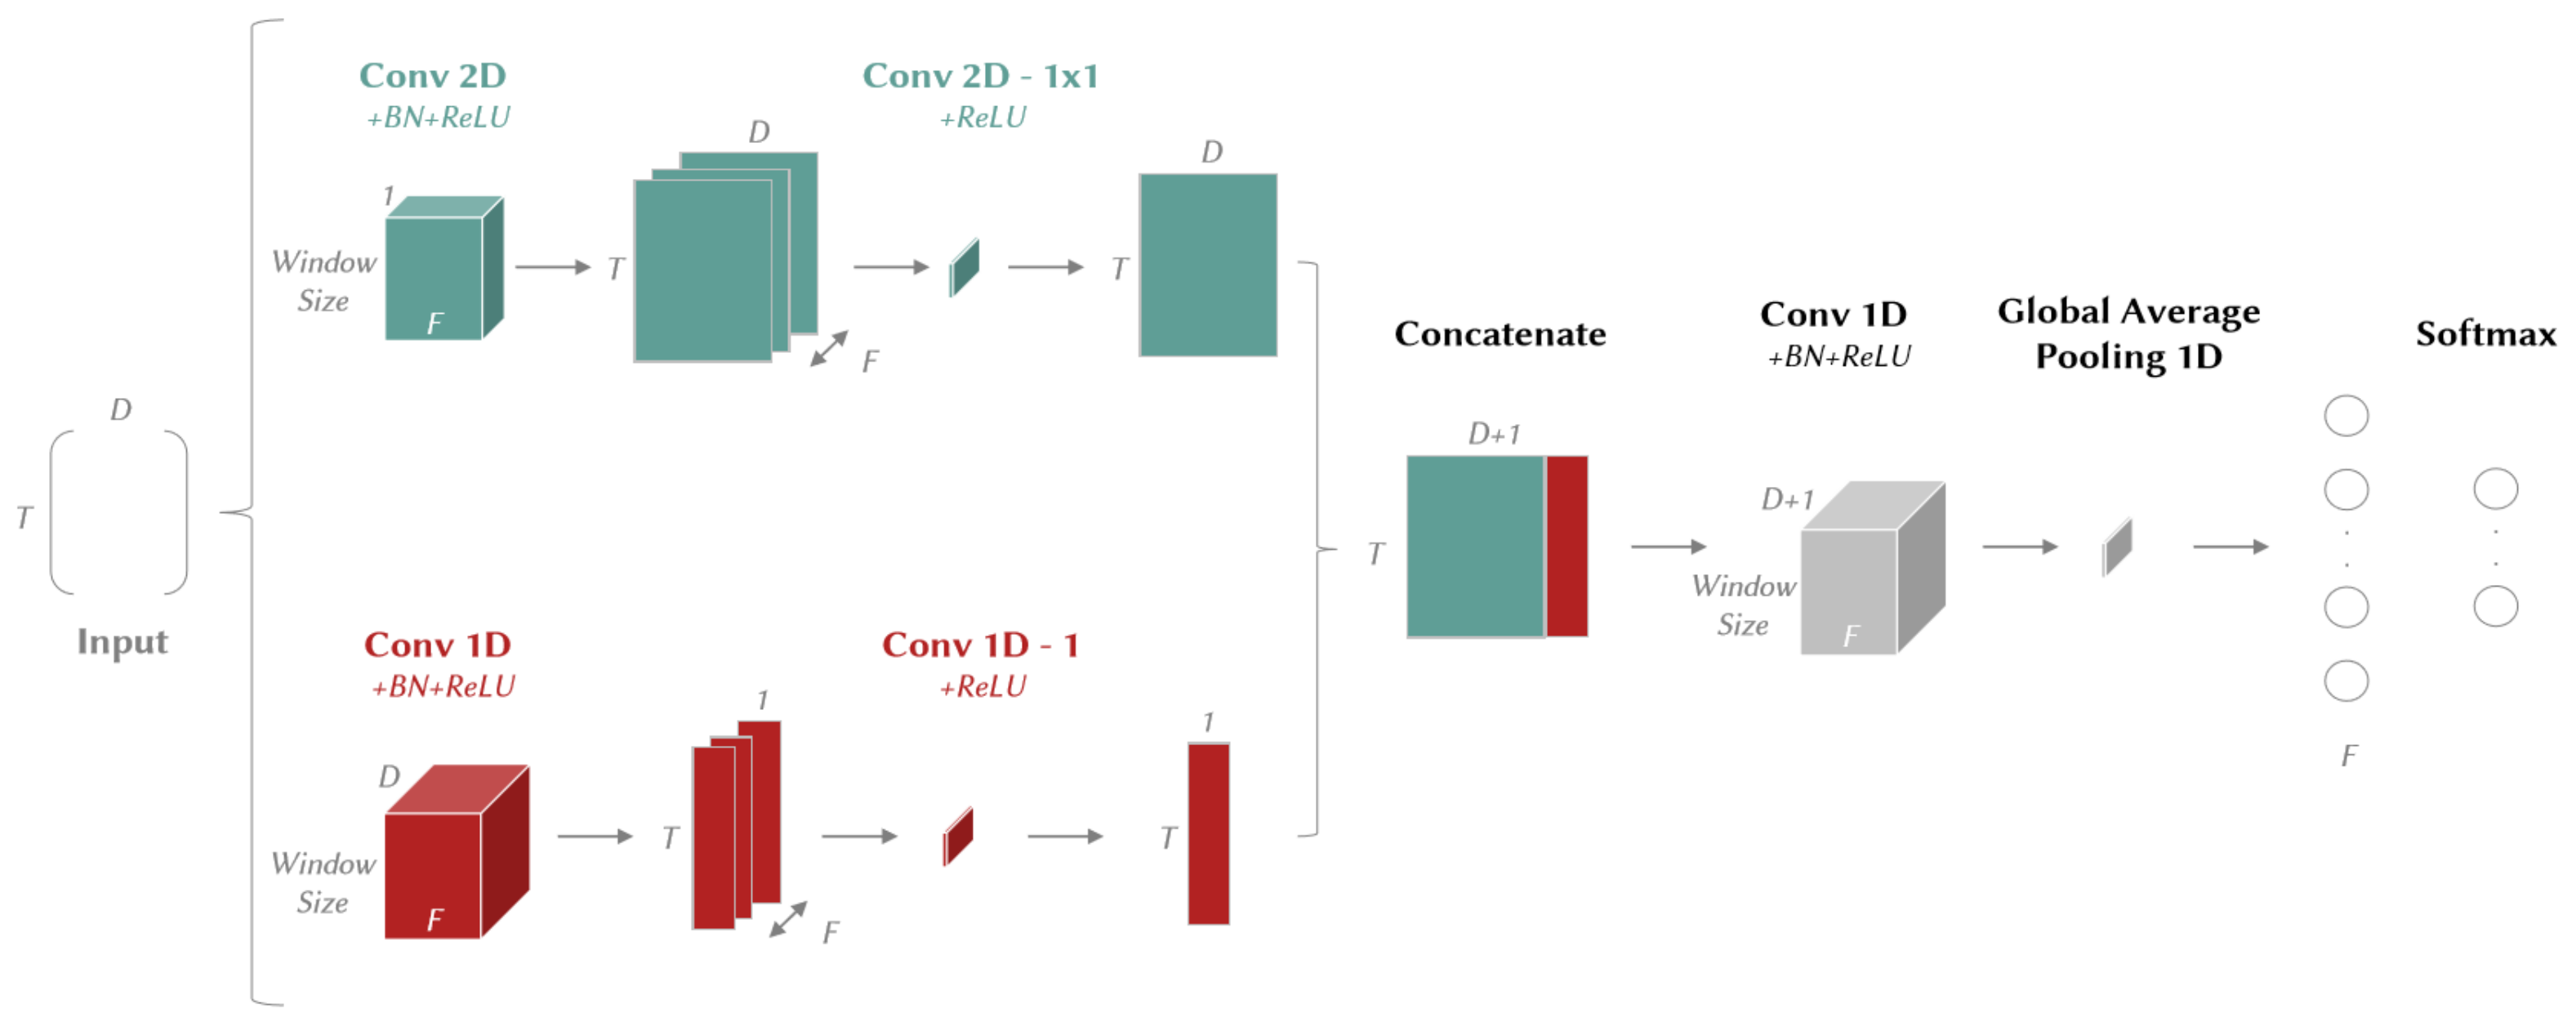
\includegraphics[width=0.7\textwidth]{files/figs/tsc/xcm.png}
  \caption{The XCM architecture with $BN$ - Batch Normalization, $D$ - number of input channels, $F$ - number of filters, $T$ - length of time series \cite{Fauvel2020}.}
  \label{fig:xcm}
\end{figure}

% \FloatBarrier

% !TEX root=../../mt-motion-analysis.tex
%!TeX spellcheck = en-US
\chapter{Methods} \label{ch:method}
\section{Overview}
In this chapter, the system for assessing POEs will be presented. This system is naturally divided into two parts where firstly the videos are analyzed. The first subsystem extracts body part coordinates of the subjects. This information is then passed to the second subsystem where it is used to calculate a score according to \cite{Nae2020b}. The data used is presented in Section \ref{sec:met-data} and the two subsystems are described in Sections \ref{sec:met-loc} and \ref{sec:met-class}, respectively.

\section{Data}\label{sec:met-data}
The data available is in the form of videos each containing one subject, recorded from a frontal view. As discussed in Chapter \ref{ch:intro}, the \gls{sls} task and the trunk, pelvis, femoral valgus, and \gls{kmfp} \glspl{poe} are evaluated. Each video contains four-five repetitions and for each repetition the \glspl{poe} above have been scored according to Table \ref{tab:poes}. Along with the \gls{poe} scores a certainty score, describing the confidence of the physiotherapist assessing the videos, is provided. This is between 0 (certain) and 2 (uncertain) and when above 0 the uncertainty direction is provided as well. This certainty score is only available for the combined (median) score for all repetitions, i.e. one certainty score per video.

In total there are labeled videos from 103 different subjects and for some of the subjects there are videos of the task performed with both right and left leg. The number of labeled repetitions per video and \gls{poe} varies slightly. This variation is due to different factors such as all subjects not performing five repetitions, or that the entire movement was not captured in the video and was thereby excluded by us.. The total amount of data for the different \glspl{poe} is summarized in Table \ref{tab:data}. From this data 22 of the repetition sequences (110 repetitions), from 22 different subjects, were put aside as a test set. The test set was chosen from the set of repetition sequences ensuring no data from the same sequence was in both the training and test data.

The label distributions can be seen in Figure \ref{fig:label-dist} and it can be noted that for all \glspl{poe} there is a slight imbalance with fewer repetitions classified as Poor. The imbalance for \gls{kmfp} is very clear with about 80\% of the data classified as Good. In the same figure the label distribution  for the test set is shown as well. For the trunk \gls{poe} it is slightly different from its overall distribution while similar for the other sets.

\begin{table}
 \centering
 \caption{Data available for the different POEs.}
 \label{tab:data}
 % \footnotesize
 % {\renewcommand{\arraystretch}{1.2}
 % {\tabulinesep=0.8mm
 \begin{tabu}[t]{cccc}
   \textbf{\gls{poe}} &
   \multicolumn{1}{c}{\begin{tabular}[c]{@{}c@{}}\textbf{Number of}\\\textbf{unique subjects}\end{tabular}} &
   \multicolumn{1}{c}{\begin{tabular}[c]{@{}c@{}}\textbf{Number of}\\\textbf{repetition sequences}\end{tabular}} &
   \multicolumn{1}{c}{\begin{tabular}[c]{@{}c@{}}\textbf{Number of}\\ \textbf{repetitions}\end{tabular}} \\ \hline \hline
   \textbf{Trunk} & 103 & 105 & 520 \\
   \textbf{Pelvis} & 103 & 105 & 519 \\
   \textbf{Femoral Valgus} & 103 & 107 & 530 \\
   \textbf{\gls{kmfp}} & 103 & 107 & 530

 \end{tabu}

\end{table}

\begin{figure}
  \centering
  \begin{subfigure}[t]{0.24\textwidth}
    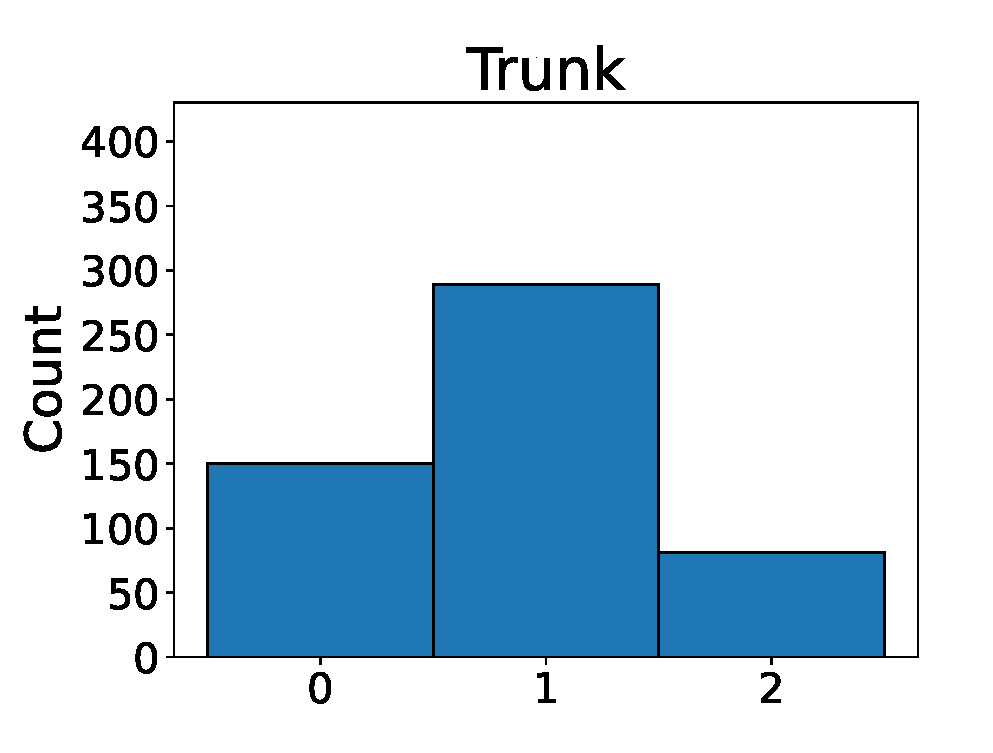
\includegraphics[width=\textwidth]{files/figs/met/trunk-label-hist.eps}
    \caption{}
    \label{fig:trunk-labels}
  \end{subfigure}
  \begin{subfigure}[t]{0.24\textwidth}
    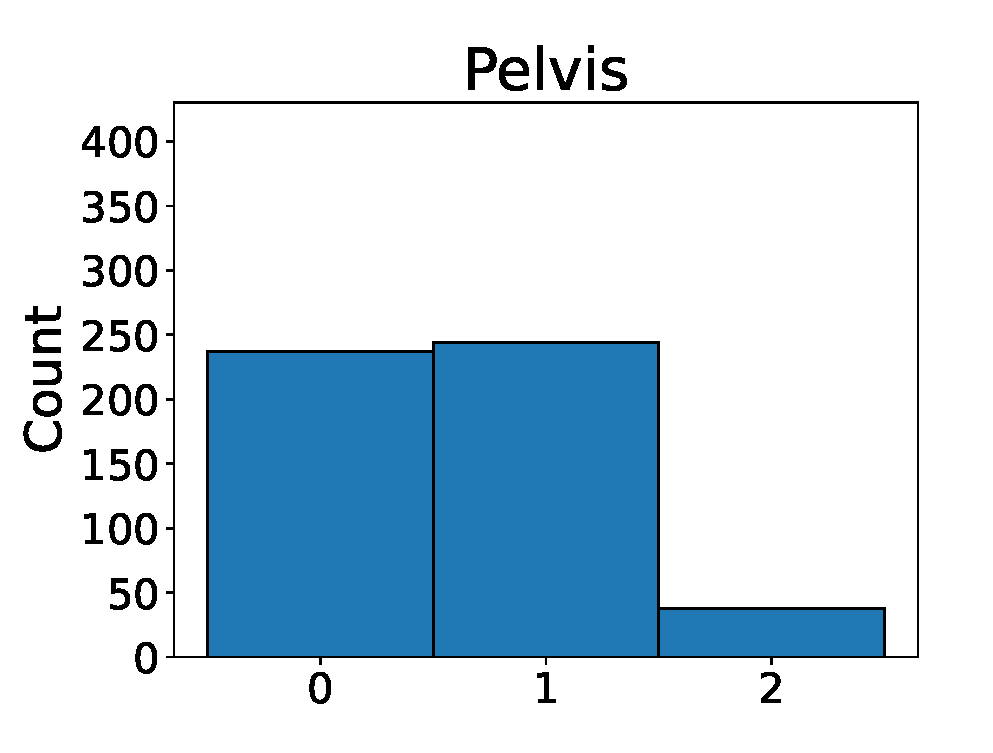
\includegraphics[width=\textwidth]{files/figs/met/pelvis-label-hist.eps}
    \caption{}
    \label{fig:pelvis-labels}
  \end{subfigure}
  \begin{subfigure}[t]{0.24\textwidth}
    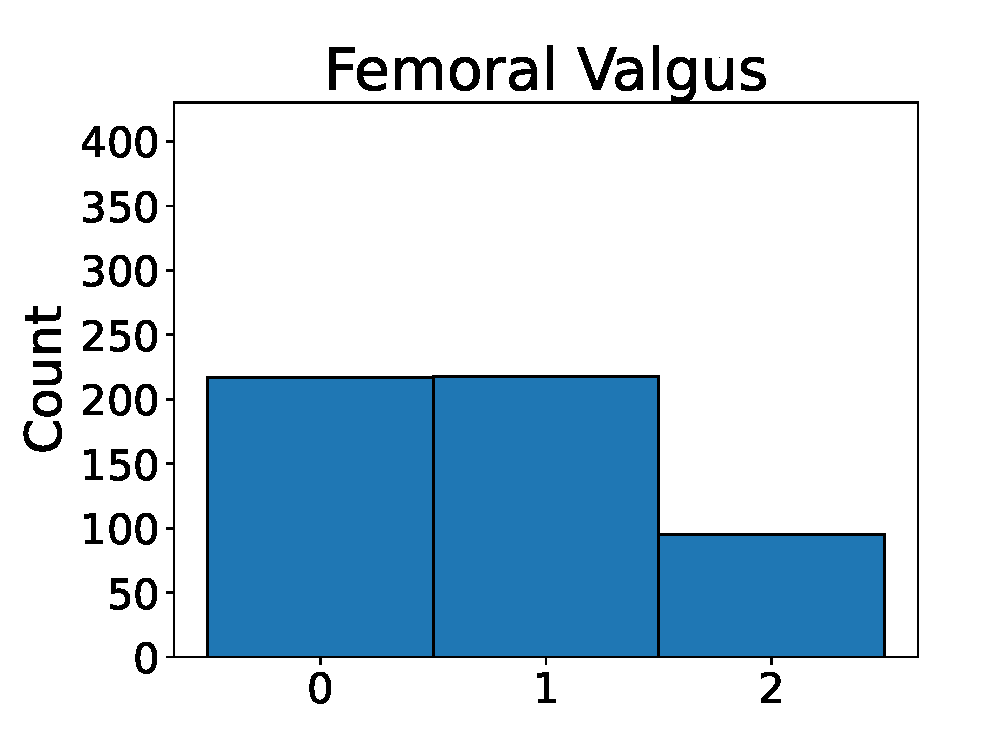
\includegraphics[width=\textwidth]{files/figs/met/femval-label-hist.eps}
    \caption{}
    \label{fig:femval-labels}
  \end{subfigure}
  \begin{subfigure}[t]{0.24\textwidth}
    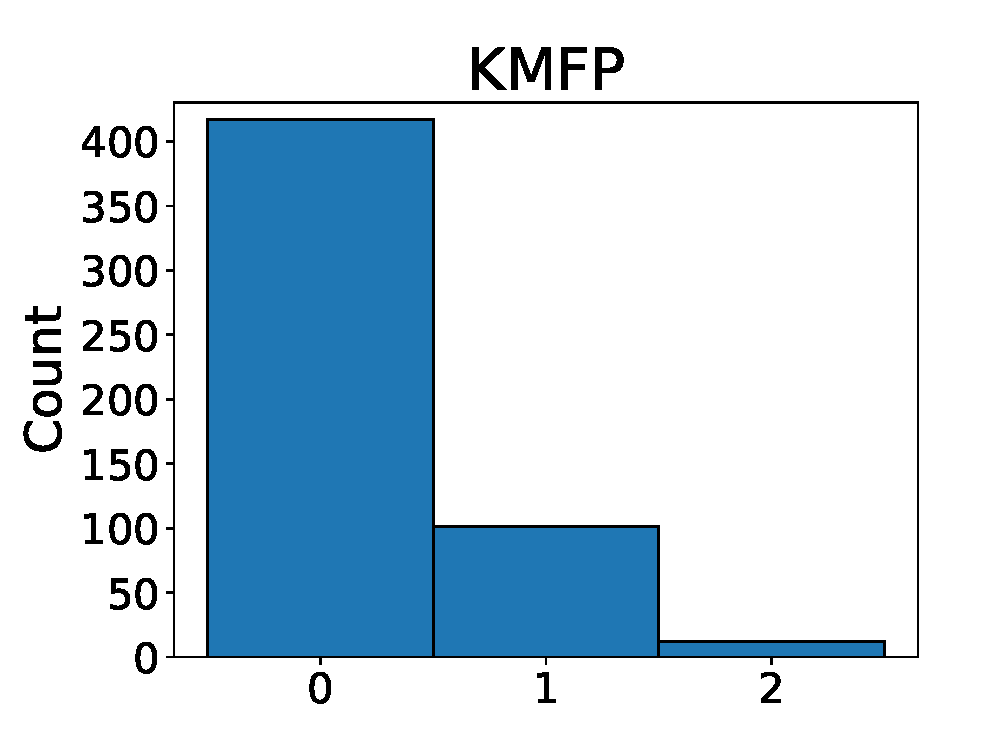
\includegraphics[width=\textwidth]{files/figs/met/kmfp-label-hist.eps}
    \caption{}
    \label{fig:kmfp-labels}
  \end{subfigure}

  \begin{subfigure}[t]{0.24\textwidth}
    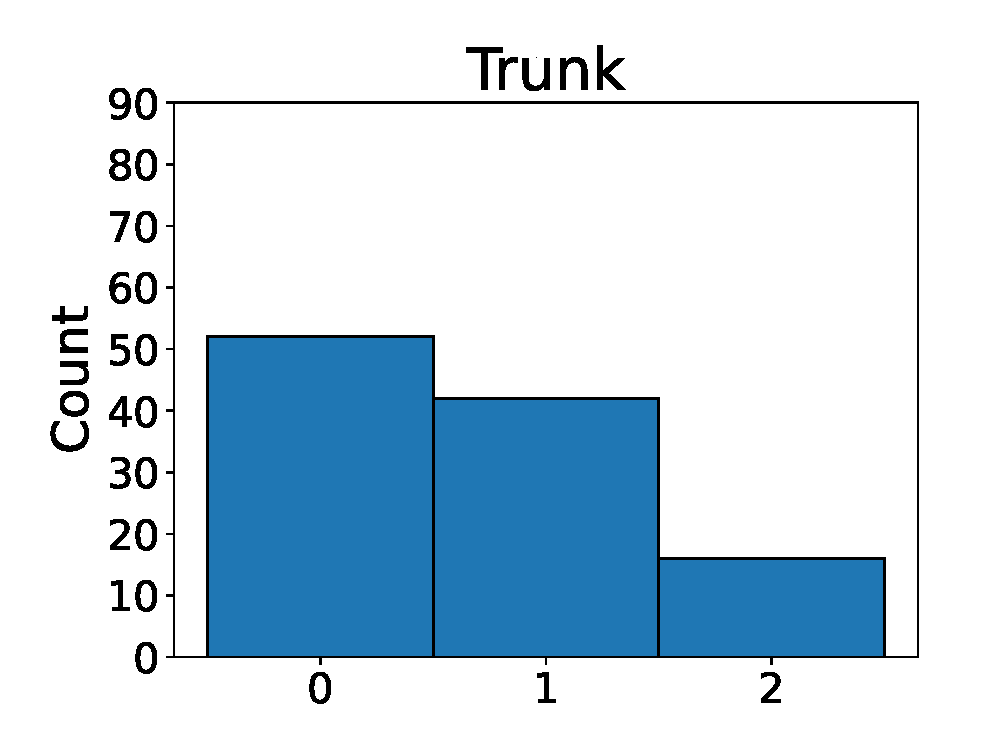
\includegraphics[width=\textwidth]{files/figs/met/trunk-test-labels.eps}
    \caption{}
    \label{fig:trunk-labels-test}
  \end{subfigure}
  \begin{subfigure}[t]{0.24\textwidth}
    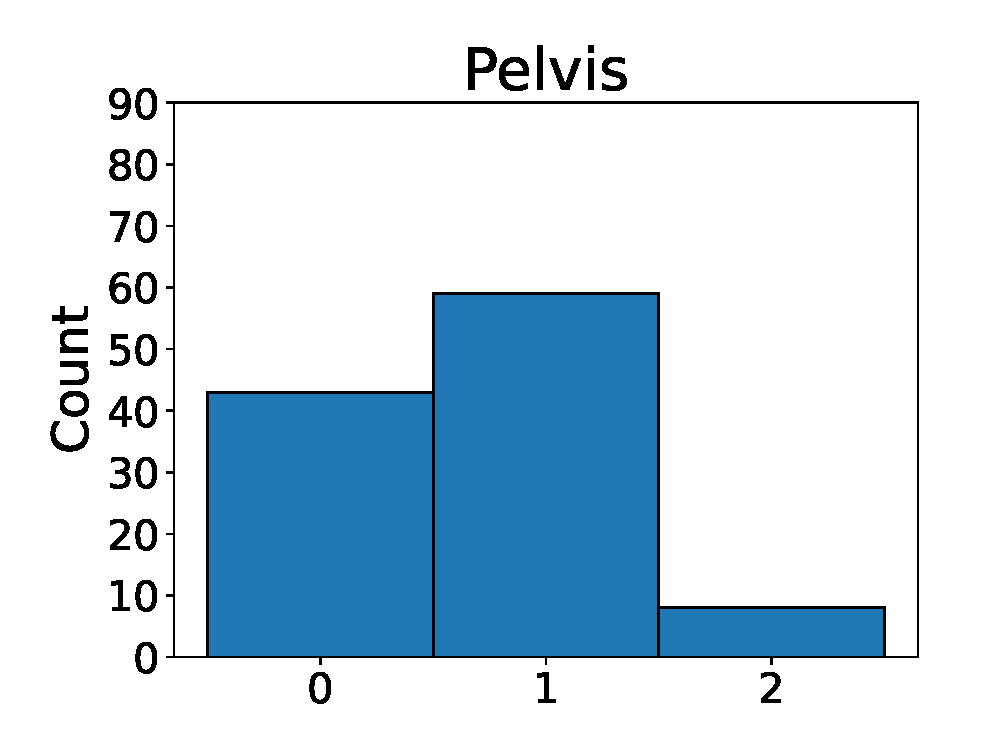
\includegraphics[width=\textwidth]{files/figs/met/pelvis-test-labels.eps}
    \caption{}
    \label{fig:pelvis-labels-test}
  \end{subfigure}
  \begin{subfigure}[t]{0.24\textwidth}
    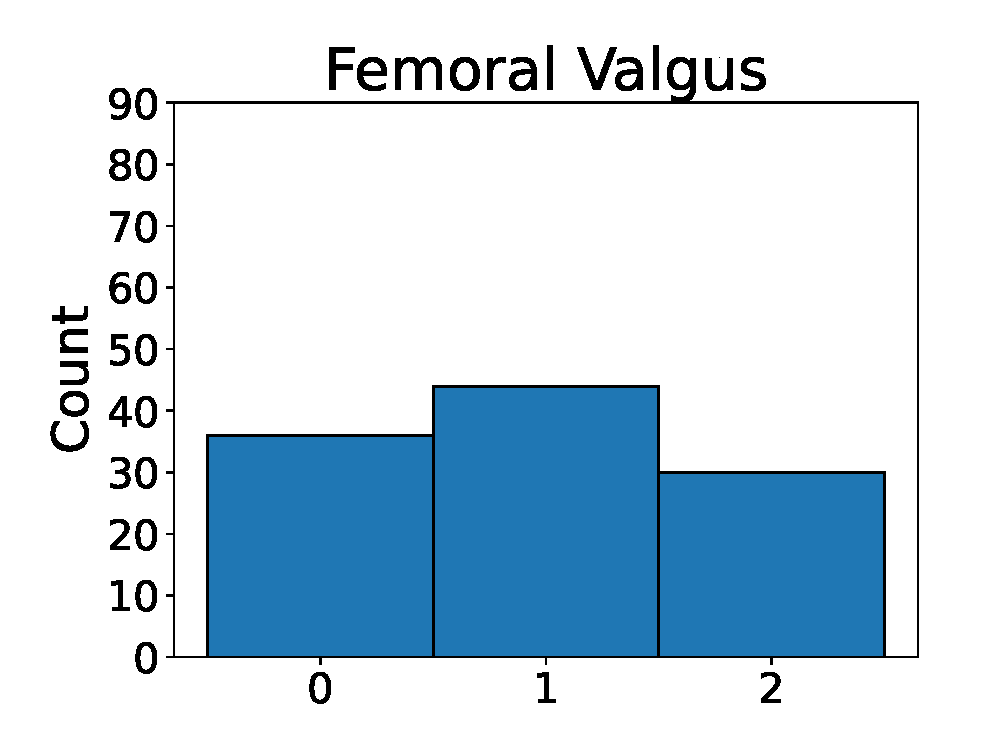
\includegraphics[width=\textwidth]{files/figs/met/femval-test-labels.eps}
    \caption{}
    \label{fig:femval-labels-test}
  \end{subfigure}
  \begin{subfigure}[t]{0.24\textwidth}
    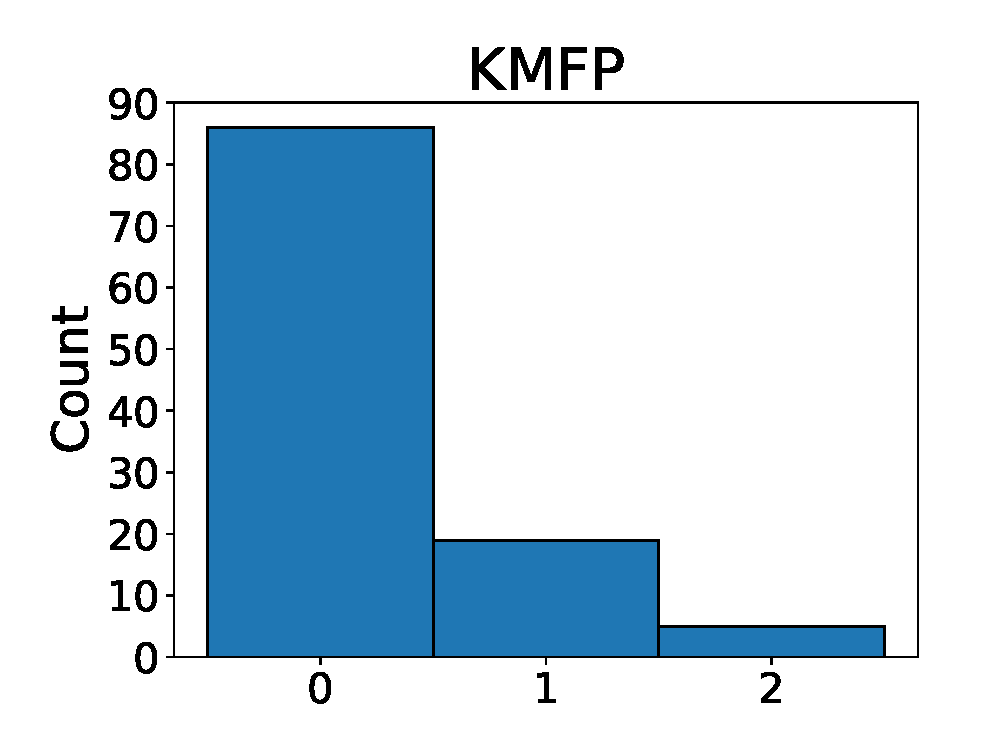
\includegraphics[width=\textwidth]{files/figs/met/kmfp-test-labels.eps}
    \caption{}
    \label{fig:kmfp-labels-test}
  \end{subfigure}

  \caption{Distributions of the labels for the available data. (a)-(d) shows distribution over all available data and (e)-(h) shows the distribution in the test set.}
  \label{fig:label-dist}
\end{figure}



\section{Body part localization} \label{sec:met-loc}
% \subsection{Preprocessing}
% ...
% rotation, flip etc
% \subsection{Pose estimation}
%The pose estimation can be seen as a feature extraction and dimensionality reduction.
The pose estimation is built around the open-source toolbox MMPose \cite{mmpose} from MMLab. Each frame is considered to be an independent image and is analyzed with a \gls{hrnet} model using the \gls{dark} extension trained on the \gls{coco}-wholebody dataset\footnote{The model used can be found here: \url{https://mmpose.readthedocs.io/en/latest/top_down_models.html}.}. Both the model and the dataset is described in Section \ref{sec:pose_estimation}. The extended wholebody dataset is used since it, along with the ankle positions, also estimates the positions of the toes and heels which contain valuable information. % \ref{sec:hrnet, sec:dark, sec:coco}.

To get comparable results some of the videos were rotated and flipped before inferring the keypoints. This was needed since the videos were recorded in different orientations and the actions were performed with different legs. The rotations were based on the orientation of the subject (position of head w.r.t. the feet) in the first frame to have it standing up in the $y$-direction. Videos where the squats were performed with the left leg were flipped around the $y$-axis to be able to use the same model for the left and right leg in a more efficient manner.

A bounding box for the subject is found using a Faster R-CNN model trained on the \gls{coco} dataset\footnote{The model used can be found here: \url{https://github.com/open-mmlab/mmdetection/tree/master/configs/faster_rcnn}.}. The content of this bounding box is resized to match the input size of the \gls{hpe} model used, 384$\times$288 pixels in our case. Each video analyzed results in sequences of $x$- and $y$-coordinates for all the keypoints in the dataset used to train the model.

%The file names contained information about which. The rotations were performed based on the position of the head with respect to the feet in the first frame.
\section{Classification} \label{sec:met-class}

\subsection{Preprocessing and creation of dataset} \label{sec:met-class-preproc}
Before assessing the \glspl{poe} based on the body part positions, a number of preprocessing steps are conducted. Firstly the data is resampled as the videos are recorded with a number of different frame rates ranging from 25 to 60 Hz. The resampling is performed using linear interpolation to a new sample frequency of 25Hz. This data is then low pass filtered through a fourth order Butterworth filter with a cutoff frequency of 5Hz. %PLOT P[ ;VERF;RING F;R FILTER? ELLER P[ FILTRERAD DATA?

While the \gls{poe} assessment is performed on a per repetition basis, the body part coordinates are extracted on a per video or repetition sequence basis. Hence, the sequences corresponding to the entire video is split up in the individual repetitions. This splitting is presented in Algorithm \ref{alg:rep} and is based on finding the edges of the peaks in specific position data. For the \gls{sls} task, the $y$-coordinate of the right shoulder is used. The number of points extracted for each repetition depends on the width of the peak. The length of the observed repetitions varies from about 1 to 8 seconds. For practical reasons, such as handling of data and training performance\footnote{All data in one batch must have the same size. Hence, to be able to train with a batch size larger than 1, which usually improves training performance \cite{Goodfellow2016}, all data in the same batch needs to have the same dimensions.}, it is desirable to save the data as multidimensional arrays with the same dimensions. Two different ways of solving this problem is evaluated, namely i) padding the sequences and use maskings for the padded samples in the models, and ii) alternate the sample frequency to thereby achieve sequences of the same length.
%Some number of points around each peak is  This is done by finding peaks in the sequences corresponding to certain body part positions. Which body part is used for this sequence splitting depends on which movement is analyzed.

\begin{algorithm}
\SetAlgoLined
% \KwResult{Write here the result }
%  initialization\;
% peaks, right\_edges, left\_edges = \textbf{find\_peaks}(sequence)\;
right\_edges, left\_edges = \textbf{find\_edges}(sequence)\;
 \For{\textup{peak, right, current\_left, next\_left} in \textup{peaks, right\_edges, left\_edges}}{
 % \For{\textup{peak, right, current\_left, next\_left} in \textup{peaks, right\_edges, left\_edges}}{
  split\_index = \textbf{mean}(right, next\_left)\;
  start = \textbf{max}(current\_left - extra\_points, 0)\;
  end = \textbf{min}(right + extra\_points, split\_index)\;
  % start = \textbf{max}(peak - max\_length/2, 0)\;
  % end = \textbf{min}(peak + max\_length/2, split\_index)\;
  \textit{repetition} = \textbf{normalize\_length}(sequence[start:end])\;
  sequence = sequence[end:]\;
 }
 \caption{Extraction of repetitions from sequences}
 \label{alg:rep}
\end{algorithm}


Finally, the data is normalized. All coordinates are moved to put the mean position of the first five right hip-samples in the origin and are scaled to set the distance between the right shoulder and right hip to one, according to

\begin{align}
  \begin{split}
    (x,y)_i &= (x,y)_i - {\mean{(x,y)}}_{rh} \\
    (x,y)_i &= \frac{(x,y)_i}{\lVert \mean{(x,y)}_{rs} \rVert_2} \qquad , \forall i
  \end{split}
  \label{eq:met-normalization}
\end{align}
where $\mean{(x,y)}_i$ denotes the mean over first five samples for body part $i$, \textit{rh} the right hip, \textit{rs} the right shoulder, and \textit{i} the different bodyparts.

After these preprocessing steps, a dataset with inputs $\in \mathbb{R}^{N \times T \times F}$ and corresponding one-hot labels $\in \mathbb{Z}_3^N$ are created. The inputs consists of $N$ multivariate time series of length $T$ with $F$ channels. These channels are a subset of the extracted $x$- and $y$-coordinates as well as angles and differences between keypoints. Which features are used and how they are chosen are presented in Section \ref{sec:met-inputs}.

\subsection{Classifiers}
For the modeling, we used ensembles of different deep learning based model architectures. The reasoning behind this was based on the results of Fawaz et al. \cite{IsmailFawaz2019ensemble}, suggesting that the output a deep learning model trained on a limited amount of data will vary based on the initial parameter values. By averaging the result over several models this variance will be reduced. Another reason for using an ensemble is, as can be seen in e.g. \cite{Bagnall2015, Lines2016}, that the combined result of many specialized models can be better than that of one more general model. %In this work it for instance mean that we can train models with the confusion-entropy loss \eqref{eq:confusion-entropy} to achieve e.g. high precision for just one class in combination with models trained with the \gls{coral} loss \eqref{eq:coral-loss} performing fairly good over all classes.

All models used have been modified to handle the padded input data discussed in Section \ref{sec:met-class-preproc}. This is done by adding masking layers setting the padded samples to zero throughout the networks, as illustrated in Figure \ref{fig:x-inception}. This reduces the impact of the padded samples to something similar to the padding performed in convolutional layers to keep the size of the feature map intact. The same mask indicates which time steps should be ignored in the \gls{gap} layer.

The models eventually used were InceptionTime (Section \ref{sec:inception-time}) with different loss functions as well as an architecture designed by us, inspired by
\gls{xcm} (Section \ref{sec:XCM}) and InceptionTime. We call this model X-InceptionTime and it is presented below.

\subsubsection{X-InceptionTime} \label{sec:xinception}
The idea with this model was to combine the explainability of XCM with the inception module from InceptionTime. This was done by separating the inputs and having individual inception modules for each input channel as can be seen in Figure \ref{fig:x-inception}. After the final module (the depth can be seen as a hyperparamtere and needs to be tuned) a bottleneck of size one is applied reducing the dimensionality of each input channel back to $T$$\times$1. The features for the individual inputs are concatenated resulting in a feature map of size $T$$\times$$F$ where each input feature is only affected by that input. This makes it possible to use \gls{grad-cam} to get a measure of the importance of each time step for each input.

\begin{figure}
  \centering
  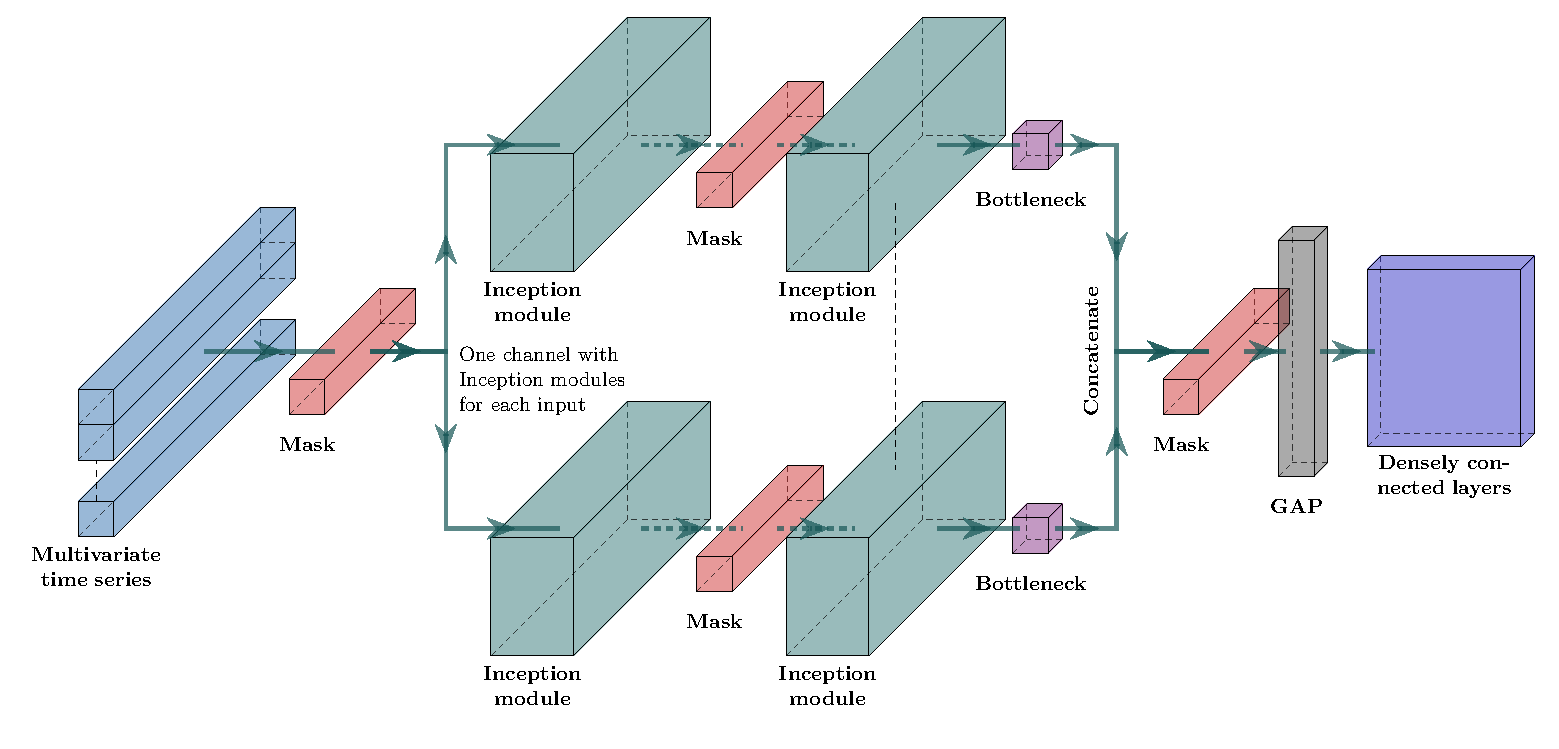
\includegraphics[width=\textwidth]{files/figs/met/x-inception-w-masks.pdf}
  \caption{The X-InceptionTime architecture developed in this work.}
  \label{fig:x-inception}
\end{figure}

The \gls{grad-cam} method is slightly modified and simplified for this model compared to what is presented in Section \ref{sec:grad-cam}, mainly due to the one dimensional data. Consider the final feature map $A$ consisting of the concatenated feature maps from the separate input channels. As mentioned above $A \in \mathbb{R}^{T \times F}$ and the aim is to find importance values for each time step in each input. With the same notations as in \eqref{eq:grad-cam}, i.e. $A_i^k$ corresponds to the activation of input $k$ at time step $i$, the \gls{grad-cam}, $M_c^k$, for class $c$ and input $k$ can be calculated as follows

\begin{align}
    \begin{split}
        w_k^c &= \frac{1}{T}\sum_{i=1}^T \frac{\partial y_c}{\partial A_i^k} \\
        M_c^k &= w_k^c A^k.
    \end{split}
    \label{eq:grad-cam-x}
\end{align}

 Compared to \eqref{eq:grad-cam} the $ReLU$ activation has been removed. This means that the importance values also contain information about which features suggesting this sample belongs to another class than $c$.

 Along with the effect of the time steps it is also possible, thanks to the \gls{gap} layer, to get a measure of the importance of each input. The importance value, $\alpha_k^c$, for input $k$ describes how much effect this input has on the classification decision. It is given by applying the \gls{grad-cam} method to the output of the \gls{gap} layer, $B$. From the feature map, $A$, this importance weight is calculated according to

 \begin{align}
   \begin{split}
      B^k &= \frac{1}{T}\sum_{i=1}^T A_i^k \\
      w_k^c &= \frac{\partial y_c}{\partial B^k} \\
      \alpha_k^c &= w_k^c B^k.
      \label{eq:input-importance}
   \end{split}
 \end{align}


\subsubsection{Ensembles} \label{sec:met-ensembles}
The ensembles used consists of multiple models whose outputs are linearly combined to form the ensemble output. As discussed above, this allows the ensemble to benefit from models optimized to perform well according to different metrics. In Section \ref{sec:met-training}, we will present how $k$-fold cross-validation was used for training and validation. This was also used for design of the ensembles.

The idea with the ensemble was to combine models performing across all classes with models with high precision for the individual classes. The models with good overall performance was in general using the \gls{coral} activation and loss. The other models were trained with the confusion entropy loss with a target confusion matrix, from which the $u_{ij}$ in \eqref{eq:confusion-entropy} comes, aiming at achieving high precision for one class and ignoring the other predictions. Examples of matrices used to find high precision models are

\noindent\begin{subequations}
\begin{minipage}{.33\textwidth}
  \begin{align}
  \label{eq:target-0}
  \begin{bmatrix}
    0.6 & 0.05 & 0.05 \\
    0 & 1 & 1\\
    0 & 1 & 1
  \end{bmatrix}
\end{align}
\end{minipage}%
\begin{minipage}{.33\textwidth}
  \begin{align}
  \label{eq:target-1}
  \begin{bmatrix}
    1 & 0 & 0 \\
    0.3 & 0.5 & 0.3\\
    0 & 0 & 1
  \end{bmatrix}
\end{align}
\end{minipage}%
\begin{minipage}{.33\textwidth}
  \begin{align}
  \label{eq:target-2}
  \begin{bmatrix}
    1 & 1 & 0 \\
    1 & 1 & 0 \\
    0.1 & 0.1 & 0.4
  \end{bmatrix}.
\end{align}
\end{minipage}
\label{eq:confusion-target}
\end{subequations}

A higher value can be seen as a reward for predictions turning up at that position in the confusion matrix and clearly the sum of the columns are not equal, meaning that the models will be biased towards certain predictions. Eq. \eqref{eq:target-0} is used for class 0 and the ones in the lower right corner in this example means that correct prediction of a 1 will give the same reward as incorrectly predicting it as a 2.
The idea behind the lower reward for correct prediction of 0 together with the small rewards for predicting it as a 1 or 2 is to classify uncertain examples as 1s or 2s. The idea for class 2, in \eqref{eq:target-2} is the same, but opposite. As the underlying scoring scale is ordinal, the same approach was not suitable for class 1. Instead a target matrix like \eqref{eq:target-1} was used. An alternative way of achieving high precision models was to tune the weight parameters $\lambda$ in the \gls{coral} loss, \eqref{eq:coral-loss}, to emphasize one of the rank predictions over the other.
Due to the significant class imbalance for the \gls{kmfp} \gls{poe} the goal for class 1 and 2 was not to achieve high precision. Instead models slightly biased towards these classes were used. This was achieved by using confusion entropy losses with target matrices shown in Appendix \ref{app:models-kmfp}.

For the ensemble output the outputs of the individual models were combined as a weighted sum, initially according to
\begin{subequations}
\begin{align}
      \mybar[0.7][1pt]{y}^{(c)} &= \sum_{i=1}^E w_i^{(c)} \widehat{y}_i^{(c)}, \\
      1 &= \sum_{i=1}^E w_i^{(c)}, \quad \forall c, \label{eq:weight-sum}
\end{align}
\end{subequations}
where $E$ denotes the number of ensembles, $\mybar[0.7][1pt]{y}$ the ensemble output, and $\widehat{y}_i$ the output of the $i$-th model.
% \begin{conditions}
%   E                   & = & number of ensembles \\
%   \mybar[0.7][1pt]{y} & = & ensemble output \\
%   \widehat{y}_i       & = & output if the $i$-th model.
% \end{conditions}

The models used were determined based on the performance during the cross-validation and the weights were chosen uniformly for all models except the high precision ones. For these the weights instead were set to zero for the classes it was not trained for. By studying the predicted output probabilities for the validation data it could be seen that they in some cases were slightly biased away from class 1. The histogram of the predicted class 1 probabilities for the Femoral Valgus data is shown in Figure \ref{fig:prob-1}. The main reason for this bias is the \gls{coral} classifier which tends to result in slightly lower predictions for intermediary classes. To prevent this from resulting in skewed combined scores (see Section \ref{sec:met-combined}) the weights for this class were increased slightly, resulting in \eqref{eq:weight-sum} summing to something greater than one for class 1. The final ensemble weights can be seen in Appendix~\ref{app:models}. The weights for all models in the ensemble were multiplied with the same factor, resulting in the adjusted histogram in Figure \ref{fig:prob-adjusted}. This adjustment shifts all probabilities, but will have a greater effect for predictions with already high probability.

\begin{figure}[h]
  \centering
  \begin{subfigure}[t]{0.45\textwidth}
  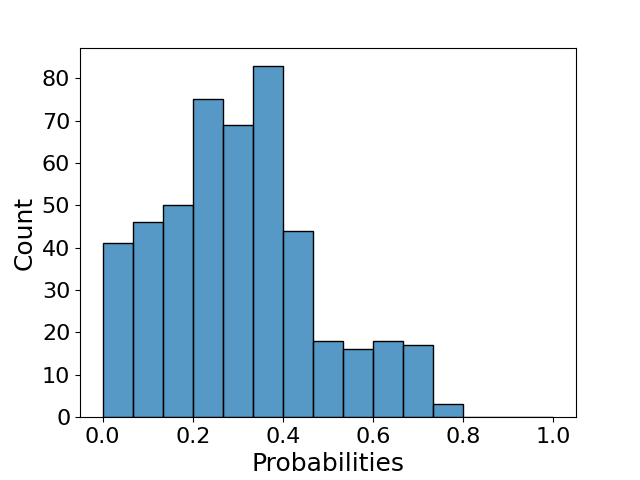
\includegraphics[width=\textwidth]{files/figs/met/probs-1.png}
  \caption{}
  \label{fig:prob-1}
\end{subfigure}
~
\begin{subfigure}[t]{0.45\textwidth}
  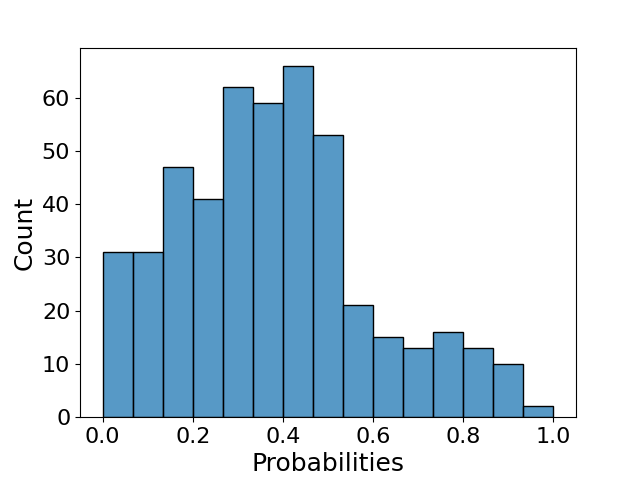
\includegraphics[width=\textwidth]{files/figs/met/probs-1-adjusted.png}
  \caption{}
  \label{fig:prob-adjusted}
\end{subfigure}
  \caption{Output probabilities for class 1 (Femoral Valgus) from the unadjusted (a) and adjusted (b) ensemble suggesting some bias away from this label.}
  \label{fig:bias-1}
\end{figure}

The ensembles used are presented in Table \ref{tab:ensemble-models}. The suffixes -coral and -conf-X indicates \gls{coral} classifiers and models trained with the confusion entropy loss, respectively. The X tells which was the high precision class. This is also used to indicate \gls{coral} models trained to achieve high precision. The depth, filter length, and number of filters for all X-InceptionTime models were 1, 31, and 32. The corresponding parameters for the InceptionTime models were 2, 31, and 128. All models use Leaky-\gls{relu} activations throughout the network. More detailed model descriptions can be found in Appendix \ref{app:models} along with its training and ensemble weights.

\begin{table}
 \centering
 \caption{Models forming the ensembles. * indicates data length normalized to 100 samples. No star means that original sample frequency (25Hz) was kept and the input data was padded to the same length. If neither coral nor conf is stated cross entropy loss is used. IT shows InceptionTime modules were used. The identifier TX, PX, FX, KX is used in Appendix \ref{app:models} where more information, such as ensemble and training weights, can be found.}
 \label{tab:ensemble-models}
 % \footnotesize
 % {\renewcommand{\arraystretch}{1.2}
 % {\tabulinesep=0.8mm
 \small
 \begin{tabu}[t]{l:l:l:l}
   \textbf{Trunk} & \textbf{Pelvis} & \textbf{Femoral Valgus} & \textbf{\gls{kmfp}} \\
   \hline \hline
   T1, IT-coral*     & P1, IT-coral*      & F1, IT-coral*    & K1, IT \\
   T2, IT-coral      & P2, IT-coral       & F2, X-IT-coral*  & K2, X-IT \\
   T3, X-IT-conf-0*  & P3, IT-conf-0*     & F3, X-IT-conf-0* & K3, X-IT-conf-0 \\
   T4, IT-conf-1*    & P4, IT-conf-1      & F4, X-IT-conf-1  & K4, IT-conf-1* \\
   T5, X-IT-coral-2* & P5, X-IT-coral-2*  & F5, X-IT-conf-2* & K5, X-IT-conf-2
 \end{tabu}
\end{table}

% The models we used in the ensembles can be divided into three categories, i) models with good overall performance, ii) models with high precision for a specific class, and iii) models with high recall for a specific class. We found regular cross entropy and \gls{coral} models be suitable for the first category. This category forms the base of the ensemble and also works as a baseline to compare against. Unless the ensemble performs better than these individual models it does not serve any purpose. The second category, models with high precision,


% coral osv. custom losses osv?

\subsection{Input selection} \label{sec:met-inputs}
To select which inputs to use when classifying the different \glspl{poe} the importance weight introduced in \eqref{eq:input-importance} was used. This was done by iteratively training models and evaluating

\begin{equation}
    W_k = \text{mean\_folds}\Big( \text{normalize}(\sum_{i=1}^N |w_{ik}^{c_i}|) \Big),
    \label{eq:feat-select}
\end{equation}
where $\text{mean\_folds}(z)$ denotes the average of $z$ over all folds, $\text{normalize}(z) = \frac{z}{\lVert z \rVert_2}$, and $c_i = \argmax(\hat{y}_i)$, i.e., i.e. the predicted class.

For each set of inputs evaluated the features corresponding to the lowest $W_k$ were removed until the performance of the model dropped significantly. This method has its drawback, the most notable being that only input features suitable for this architecture will be found. This model does not consider interaction between different features directly as the inputs are kept separate throughout the network, hence features important through such interactions might not be deemed important. This was somewhat circumvented by validating the reduced input features on other model architectures as well, allowing this methodical way of finding suitable inputs. The inputs used for the different \glspl{poe} are presented in Table \ref{tab:model-inputs}.



\begin{table}
  \caption{Inputs to the models classifying the different POEs. If the task was performed with the left leg the video has been mirrored, as described in Section \ref{sec:met-loc}.}
  \label{tab:model-inputs}
    \begin{center}
        \tabulinesep=0.8mm
        \begin{minipage}[t]{0.25\textwidth}
          \begin{tabu}[t]{l}
            \textbf{Trunk} \\ \hline \hline
            Left shoulder - $x$\\
            Right shoulder - $x$\\
            Right shoulder - $y$\\
            Left hip - $x$\\
            Left hip - $y$\\
            Right hip - $x$\\
            \multicolumn{1}{l}{\begin{tabular}[l]{@{}l@{}}Difference: right\\ hip and knee - $x$\end{tabular}}
          \end{tabu}
        \end{minipage}%
        \begin{minipage}[t]{0.25\textwidth}
          \begin{tabu}[t]{l}
            \textbf{Pelvis} \\ \hline \hline
            Right shoulder - $x$\\
            Right shoulder - $y$\\
            Right hip - $x$\\
            Right hip - $y$\\
            Left hip - $y$\\
            \multicolumn{1}{l}{\begin{tabular}[l]{@{}l@{}}Difference: right\\ hip and knee - $x$\end{tabular}}\\
            \multicolumn{1}{l}{\begin{tabular}[l]{@{}l@{}}Difference: right\\ knee and toes - $x$\end{tabular}}
          \end{tabu}
        \end{minipage}%
        \begin{minipage}[t]{0.25\textwidth}
          \begin{tabu}[t]{l}
            \textbf{Femoral Valgus} \\ \hline \hline
            Right shoulder - $x$\\
            Right hip - $x$\\
            Right knee - $y$\\
            \multicolumn{1}{l}{\begin{tabular}[l]{@{}l@{}}Angle: right\\ knee and ankle\end{tabular}}
          \end{tabu}
        \end{minipage}%
        \begin{minipage}[t]{0.25\textwidth}
          \begin{tabu}[t]{l}
            \textbf{\gls{kmfp}} \\ \hline \hline
            Left shoulder - $y$\\
            Right hip - $y$\\
            \multicolumn{1}{l}{\begin{tabular}[l]{@{}l@{}}Angle: right\\ ankle and toes\end{tabular}}\\
            \multicolumn{1}{l}{\begin{tabular}[l]{@{}l@{}}Difference: right\\ hip and knee - $x$\end{tabular}} \\
            \multicolumn{1}{l}{\begin{tabular}[l]{@{}l@{}}Difference: right\\ knee and ankle - $x$\end{tabular}} \\
            % \multicolumn{1}{l}{\begin{tabular}[l]{@{}l@{}}Difference: right\\ knee and ankle - $x$\end{tabular}}
          \end{tabu}
        \end{minipage}%
    \end{center}
\end{table}

\subsection{Training} \label{sec:met-training}
We used 10-fold cross-validation on the training set for the development of the models and ensembles. The amount of data used for training ranges from 74-77 sequences of repetitions and 369-380 repetitions for the different folds and \glspl{poe}. Like the test set, the folds were created such that no repetitions from the same subject were in both the test and validation set. For all models a batch size of 32, a learning rate of $5 \times 10^{-3}$, the Adam optimizer, and early stopping was used. The learning rate was also reduced by a factor of 0.85 every 50th epoch. The training was performed on Nvidia Tesla T4 and V100 \glspl{gpu}.

% \subsection{Choice of input features}

\subsection{Combined score} \label{sec:met-combined}
The eventual score in the method proposed by Nae et al. \cite{Nae2020b} is the combined assessments of all the repetitions. This score is formed as the median of the repetition scores. We propose to do this by averaging the ensemble outputs instead and chose the class with highest average probability over all repetitions. This means that a repetition classified with some uncertainty will affect the combined score less than a certain one. By evaluating the distributions for the ensemble outputs (Appendix \ref{app:val-hists}) it is also possible to introduce thresholds for both the combined score and the repetition score. For the repetition predictions the probability was set to 0 if the prediction was below 0.2. The validation data also suggests that the combined probability should work as an indicator of the certainty of the prediction. It could also be used to introduce a threshold, e.g. ignoring predictions with a probability below 0.4. Such a threshold would be a trade-of between accuracy and number of ignored subjects.

% !TEX root=../../mt-motion-analysis.tex
\chapter{Results and Discussion} \label{ch:results}
\section{Body part localization}
The pose estimation was reliable as long as body parts were not occluded. Figure \ref{fig:occluded} shows a sequence of frames from which it is clear that all body parts except the right foot are found accurately. This figure also suggests this video was not recorded from straight ahead. This is a problem as the plane with the the coordinates will be slightly rotated, resulting in distorted body part positions.

{\addtolength{\textfloatsep}{-0.2in}
\begin{figure}[h]
  \centering
  \begin{subfigure}[t]{0.22\textwidth}
    \centering
    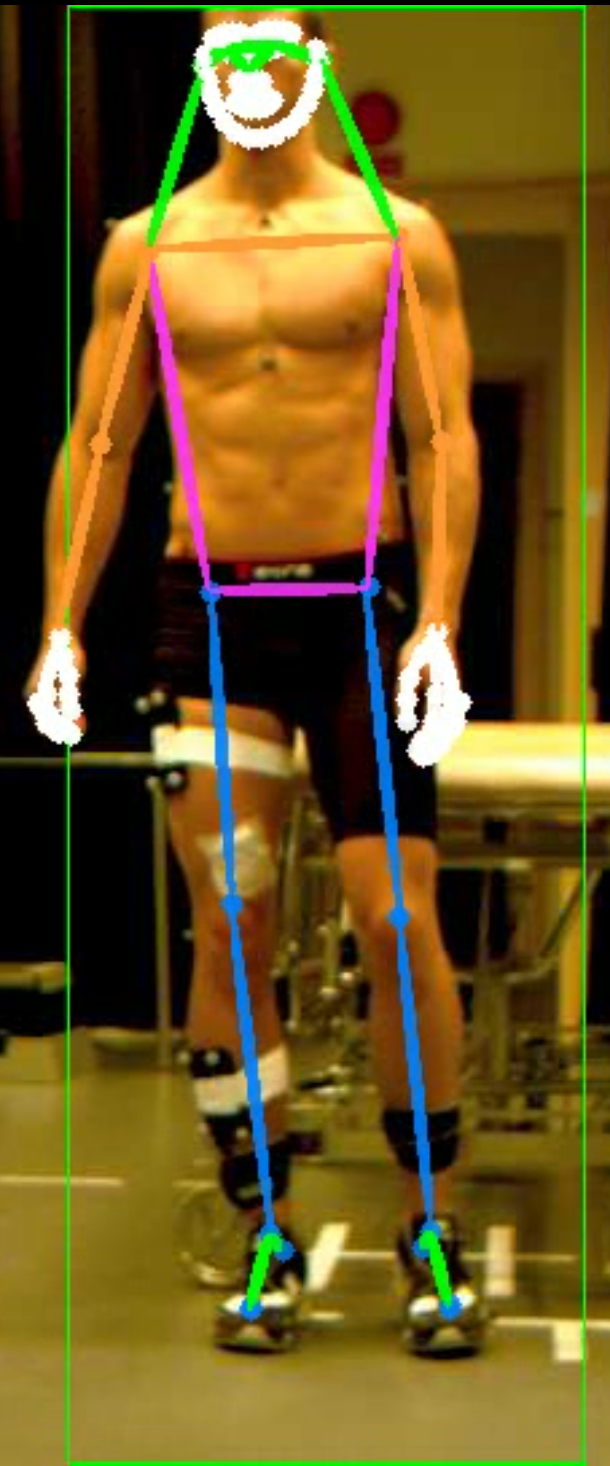
\includegraphics[height=1.3\textwidth]{files/figs/res/hpe/36-1.png}
    \caption{}
  \end{subfigure}
  ~
  \begin{subfigure}[t]{0.22\textwidth}
    \centering
    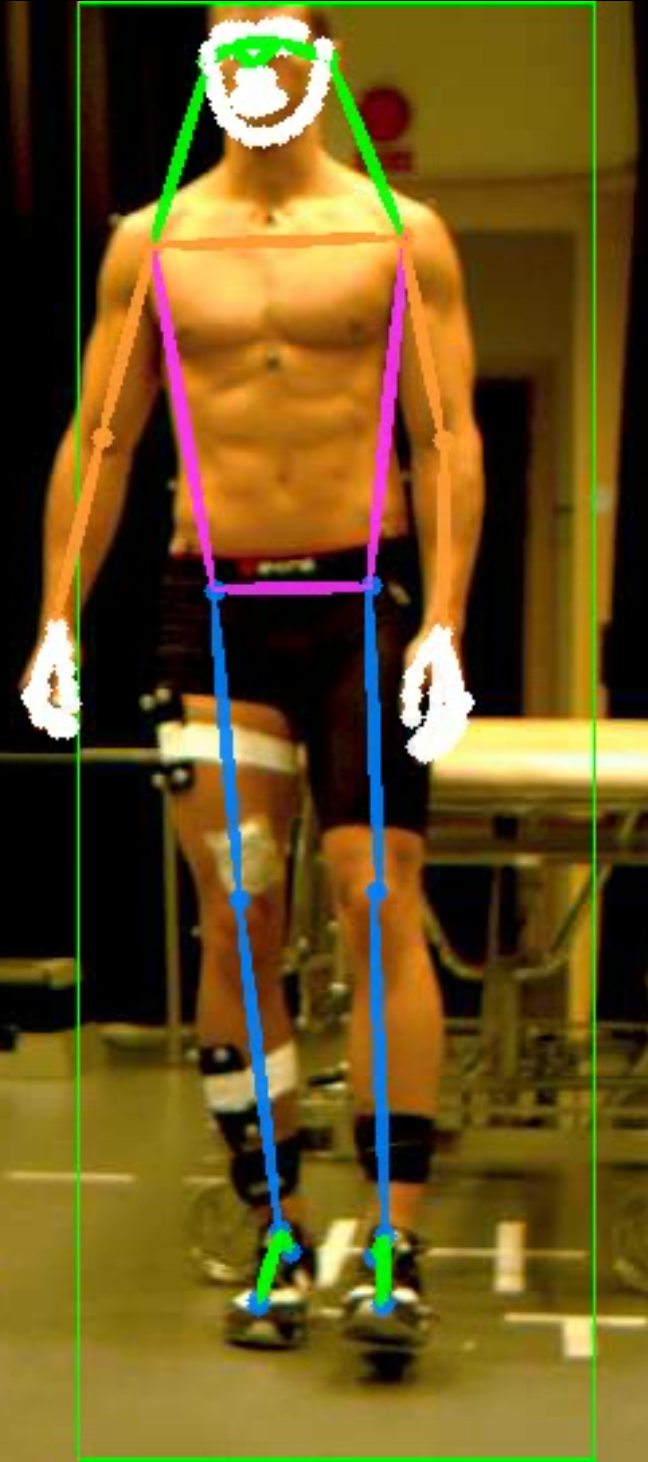
\includegraphics[height=1.3\textwidth]{files/figs/res/hpe/36-2.png}
    \caption{}
  \end{subfigure}
  ~
  \begin{subfigure}[t]{0.22\textwidth}
    \centering
    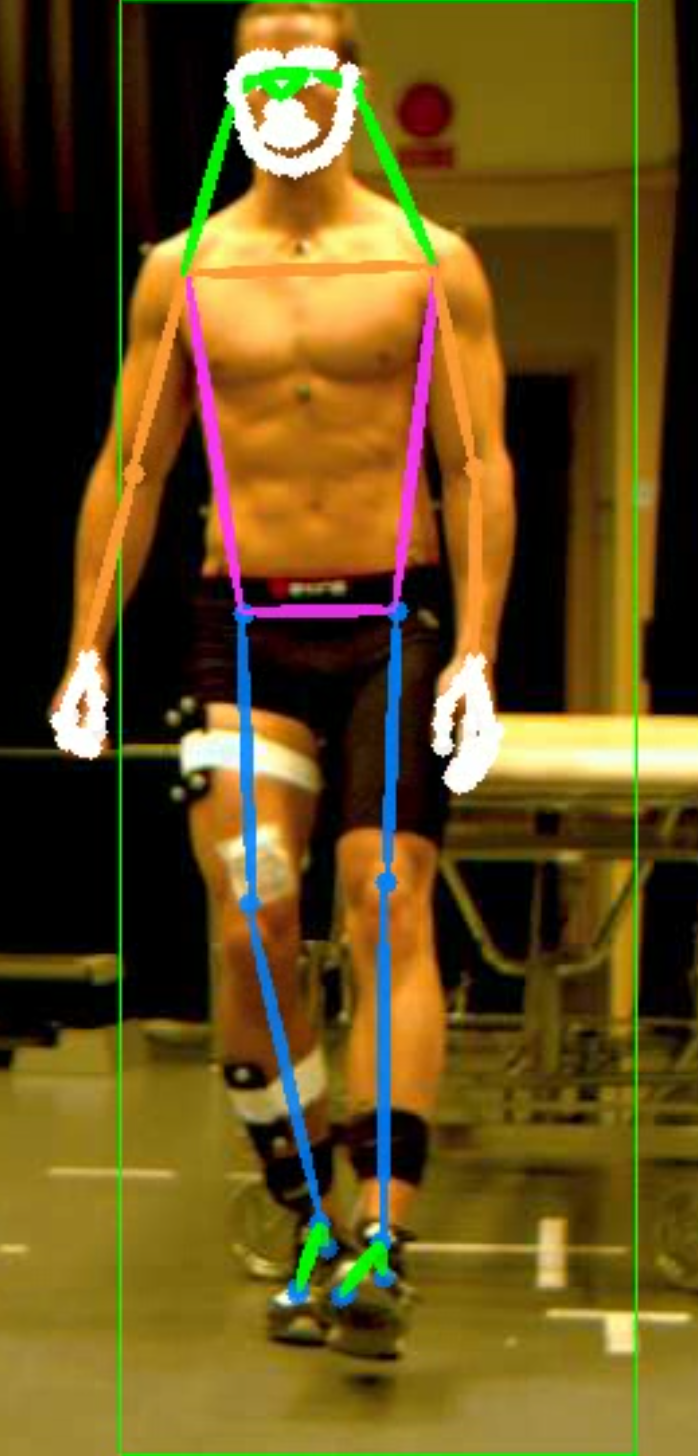
\includegraphics[height=1.3\textwidth]{files/figs/res/hpe/36-3.png}
    \caption{}
  \end{subfigure}
  ~
  \begin{subfigure}[t]{0.22\textwidth}
    \centering
    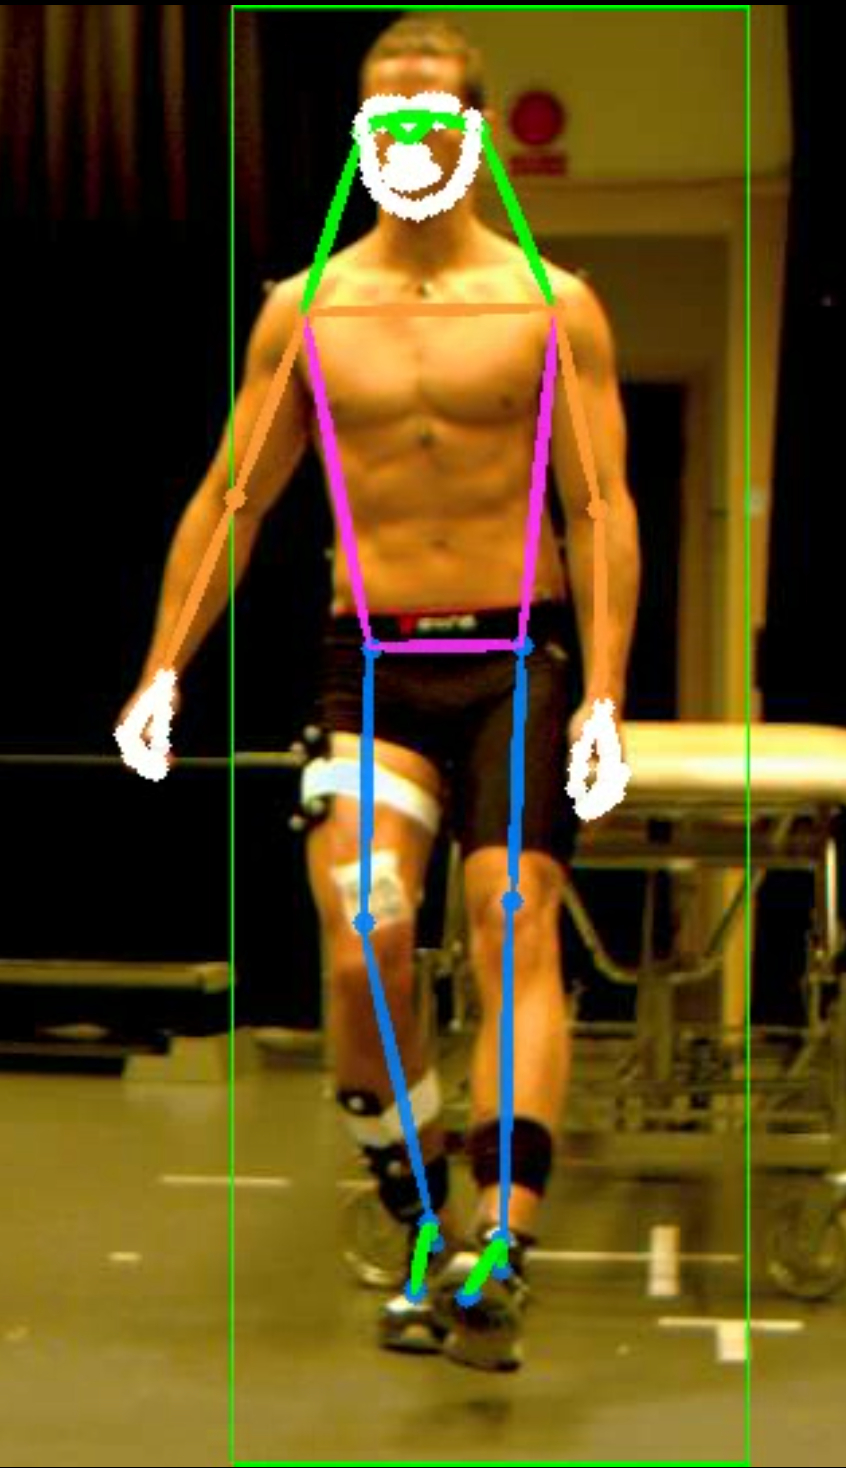
\includegraphics[height=1.3\textwidth]{files/figs/res/hpe/36-4.png}
    \caption{}
  \end{subfigure}

  \begin{subfigure}[t]{0.22\textwidth}
    \centering
    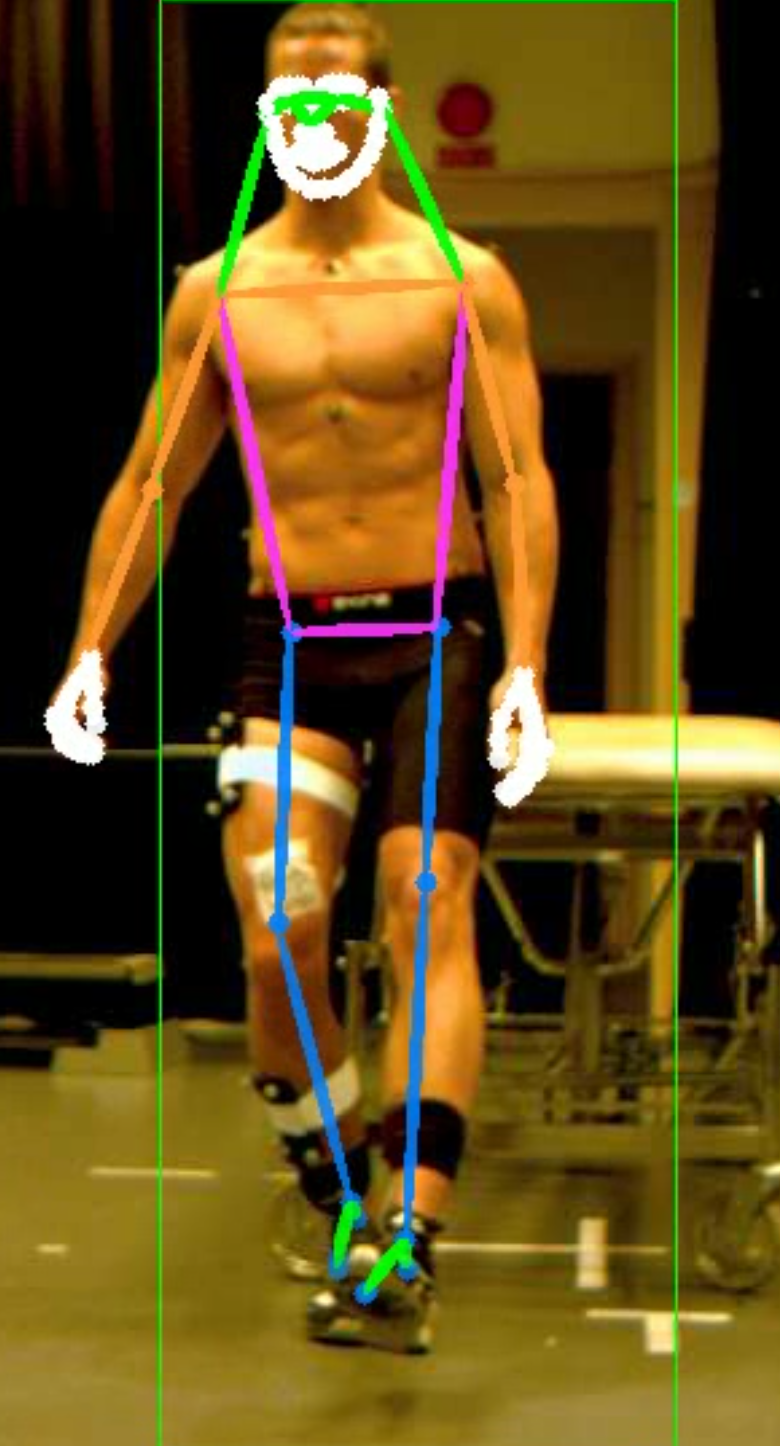
\includegraphics[height=1.3\textwidth]{files/figs/res/hpe/36-5.png}
    \caption{}
  \end{subfigure}
  ~
  \begin{subfigure}[t]{0.22\textwidth}
    \centering
    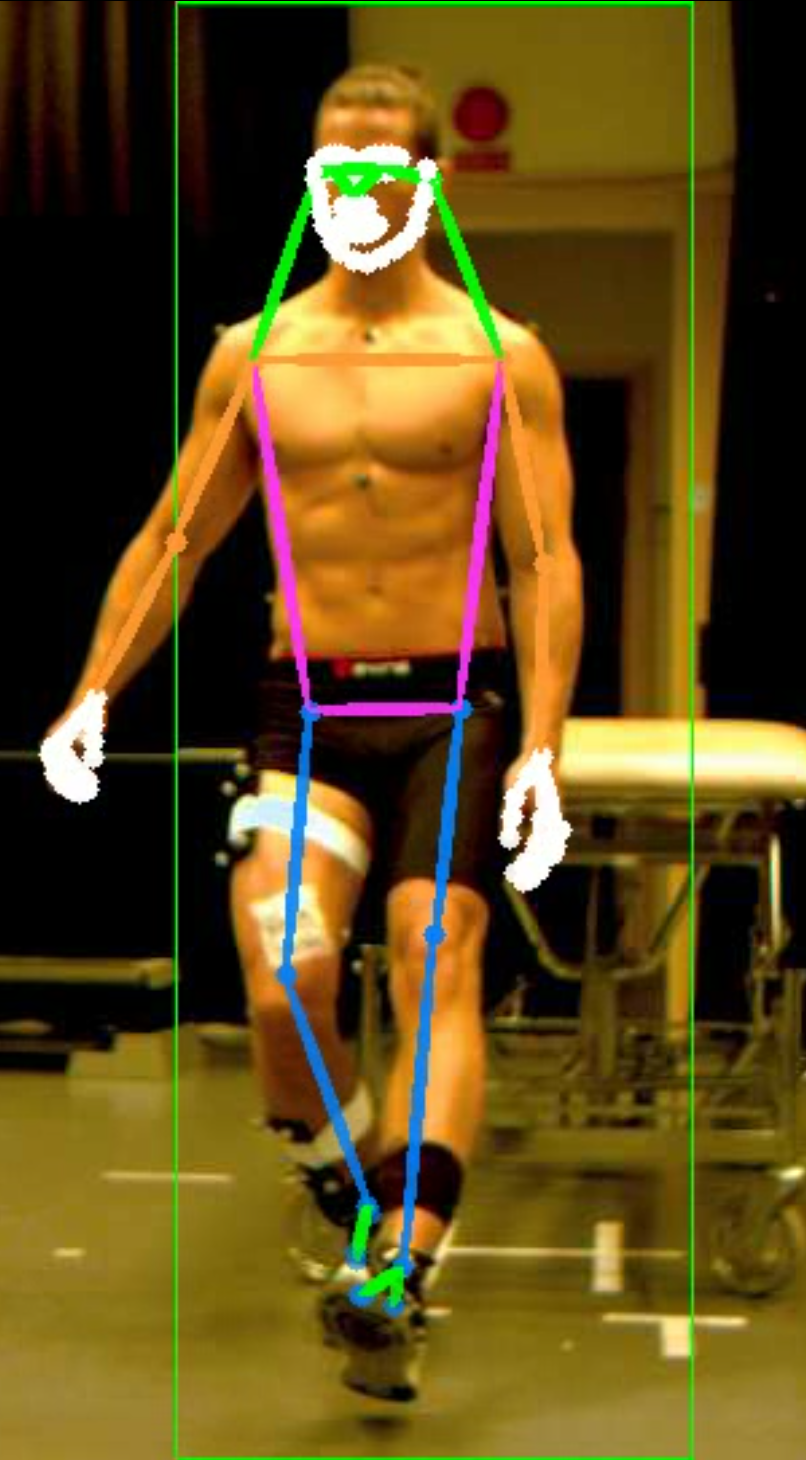
\includegraphics[height=1.3\textwidth]{files/figs/res/hpe/36-6.png}
    \caption{}
  \end{subfigure}
  ~
  \begin{subfigure}[t]{0.22\textwidth}
    \centering
    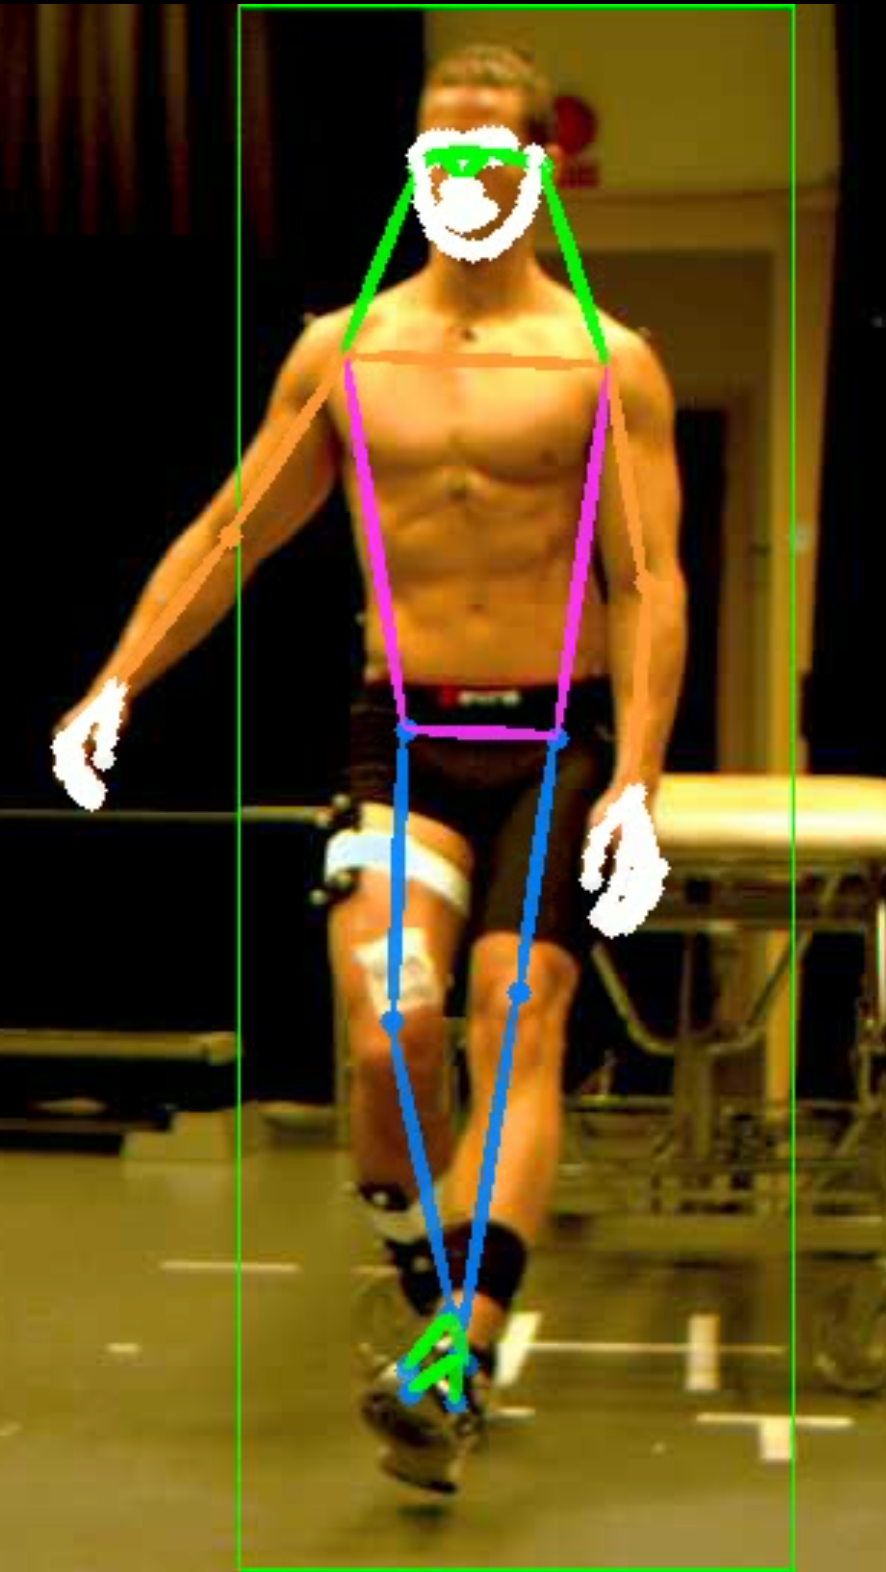
\includegraphics[height=1.3\textwidth]{files/figs/res/hpe/36-7.png}
    \caption{}
  \end{subfigure}
  ~
  \begin{subfigure}[t]{0.22\textwidth}
    \centering
    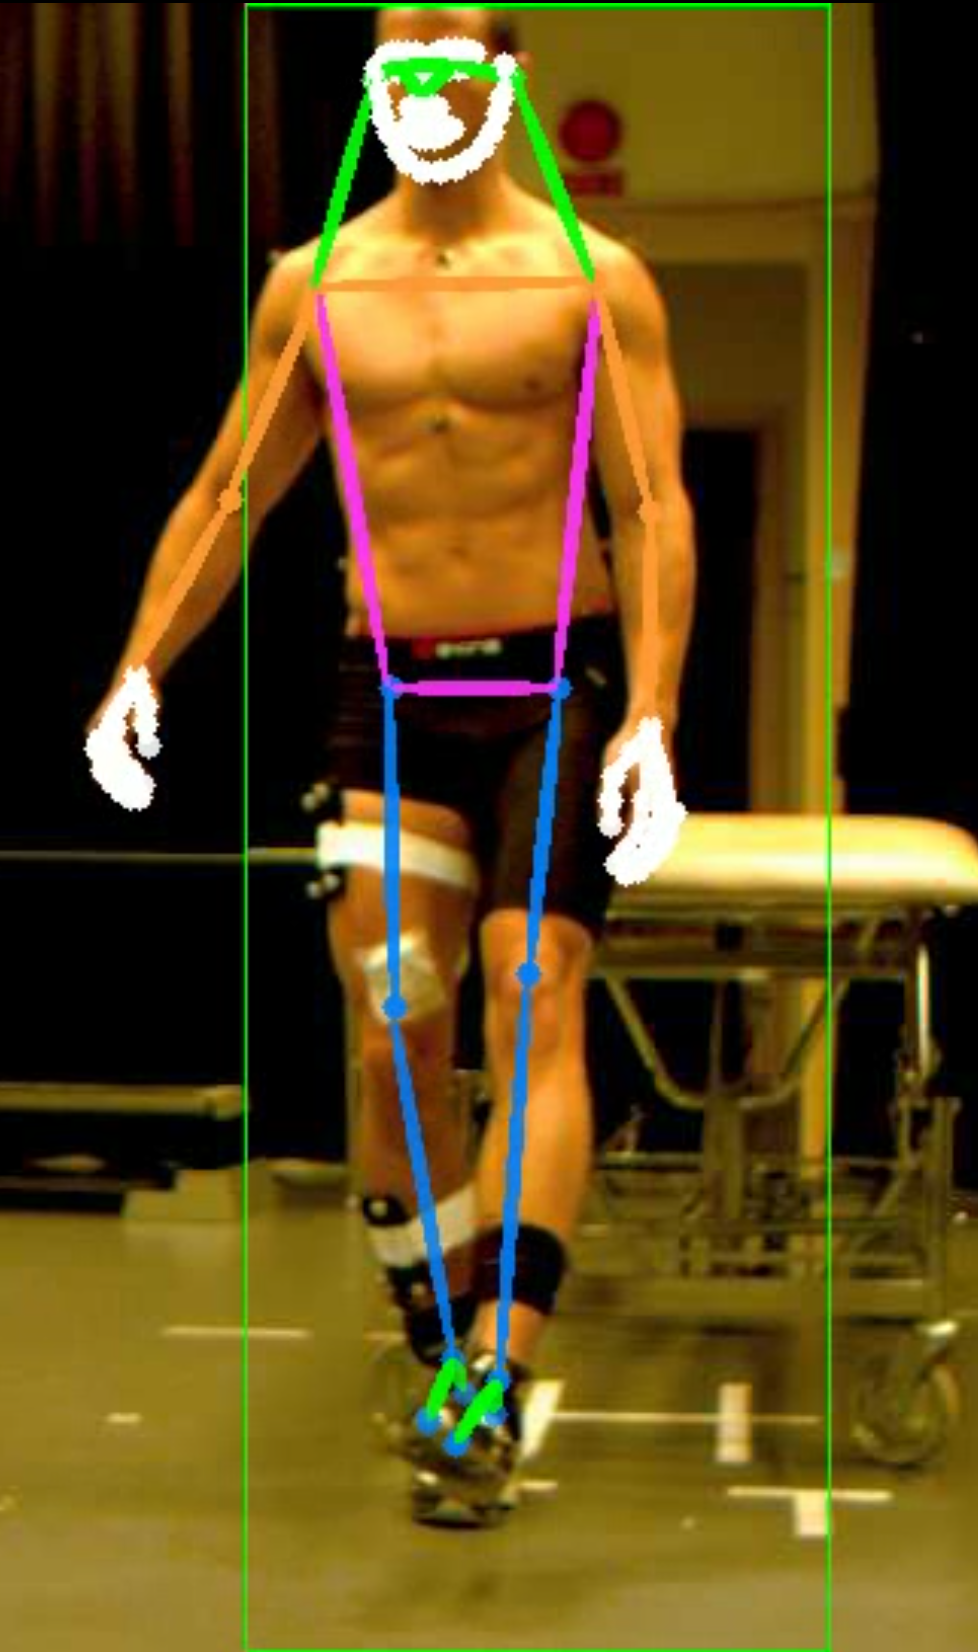
\includegraphics[height=1.3\textwidth]{files/figs/res/hpe/36-8.png}
    \caption{}
  \end{subfigure}

  \caption{Frames from video where the right foot is occluded (c)-(h).}
  \label{fig:occluded}
\end{figure}
}
% + ta fram lite resultat fr[n 3d-data???
% om jag f[r tag p[ mer data att validera mot? annars hur?

\FloatBarrier
\section{Classification}
The figures and results presented in this section are generated by models and ensembles trained according to the cross validation strategy described in Section \ref{sec:met-training} and evaluated on the test set. This results in 10 sets of models trained on slightly different data.

\subsection{Baseline results}
The repetition accuracy and F1 scores for the baseline methods presented in Section~\ref{sec:met-baseline} are shown in Table~\ref{tab:baseline-results}.

\begin{table}[h]
  \centering
  \caption{Baseline results for the different POEs for the classification of the individual repetitions. The results are the mean from the 10 folds $\pm$ the corresponding standard deviations. The F1 score is macro averaged.}
  \label{tab:baseline-results}
  \footnotesize
  {\tabulinesep=1mm
  \begin{tabu}[c]{|c||c|c||c|c||c|c||c|c|}
    \hline
     \multirow{2}{*}{}& \multicolumn{2}{c||}{\textbf{Trunk}} & \multicolumn{2}{c||}{\textbf{Pelvis}} & \multicolumn{2}{c||}{\textbf{Femoral Valgus}} & \multicolumn{2}{c|}{\textbf{\gls{kmfp}}} \\ \cline{2-9}
    & SVM & LDA & SVM & LDA & SVM & LDA & SVM & LDA \\ \hline %\hline
    Acc(\%) & {\footnotesize 35.3$\pm$5.2&45.2$\pm$5.4&52.3$\pm$4.3&46.2$\pm$3.9&38.6$\pm$3.6 &42.1$\pm$3.5&78.7$\pm$5.8&53.7$\pm$6.8}\\ \hline
    F1(\%) & {\footnotesize 17.3$\pm$1.9&41.5$\pm$5.5&35.5$\pm$3.1&37.9$\pm$3.0&29.6$\pm$2.6&40.6$\pm$3.9&36.7$\pm$2.4&47.1$\pm$9.2}\\ \hline
  \end{tabu}
  }

\end{table}

\subsection{Trunk}
Figure \ref{fig:trunk-cnf-reps}} shows the confusion matrix summarizing the classifications of the individual repetitions made by the ensemble presented in Table \ref{tab:ensemble-models} and Appendix \ref{app:models}.
Each entry in the matrix is the mean along with the standard deviation for models from the 10 folds. Figures \ref{fig:trunk-cnf-comb} and \ref{fig:trunk-cnf-comb-th} shows the corresponding matrices for the combined scores, with and without the threshold suggested in Section~\ref{sec:met-combined}. Figure \ref{fig:trunk-cnf-ignored} shows how the samples ignored due to the threshold were classified.
These results are also summarized as accuracy, F1 scores, precision, and recall in Table \ref{tab:trunk-results}. This table also shows the model performance for the data with different label certainty, specified by the physiotherapist labeling the data. Histograms for these metrics are shown in Figure \ref{fig:trunk-hist-results} along with the corresponding metrics for the individual models in the ensemble (high precision models are not shown as they only predict one label).

\begin{table}[h]
  \centering
  \caption{Results of the ensemble for the trunk POE. Rep., Comb., and Thresh. represents the results for the repetitions, combinations, and combinations with thresholds, respectively. The Certainties columns show the results making up the Comb. column, but for the certainty levels of the expert labeling the data. These ranges from certain (0) to uncertain (2), the variable $n$ shows how many datapoints each category contains. All results are the mean from the 10 folds $\pm$ the corresponding standard deviations. F1, recall, and precision are macro averaged.}
  \label{tab:trunk-results}
  \small
  \begin{tabu}[c]{|c|c|c|c||c|c|c|}
    \hline
    & \multirow{2}{*}{\textbf{Rep.}} & \multirow{2}{*}{\textbf{Comb.}} & \multirow{2}{*}{\textbf{Thresh.}} & \multicolumn{3}{c|}{\textbf{Certainties}}\\ \cline{5-7}
    & & & &0($n$=15)&1($n$=6)&2($n$=1)\\ \hline
    Accuracy (\%)   &73.7$\pm$4.5&75.0$\pm$7.9&\textbf{80.0$\pm$7.8}&
                    81.3$\pm$7.1&56.7$\pm$15.2&textbf{90.0$\pm$30.0}\\ \hline
    F1 score (\%)   &73.1$\pm$3.4&75.0$\pm$5.8&\textbf{79.9$\pm$8.9}&
                    80.4$\pm$7.1&25.8$\pm$6.3&textbf{90.0$\pm$30.0}\\ \hline
    Recall (\%)     &73.3$\pm$3.7&76.7$\pm$3.8&\textbf{81.6$\pm$7.2}&
                    \textbf{81.1$\pm$5.0}&28.0$\pm$11.0&30.0$\pm$10.0\\ \hline
    Precision (\%)  &76.7$\pm$4.1&78.7$\pm$5.2&\textbf{83.0$\pm$6.8}&
                    \textbf{84.9$\pm$5.9}&28.9$\pm$6.8&30.0$\pm$10.0\\ \hline

  \end{tabu}
\end{table}

\begin{figure}[h]
  \centering
  \begin{subfigure}[t]{0.48\textwidth}
      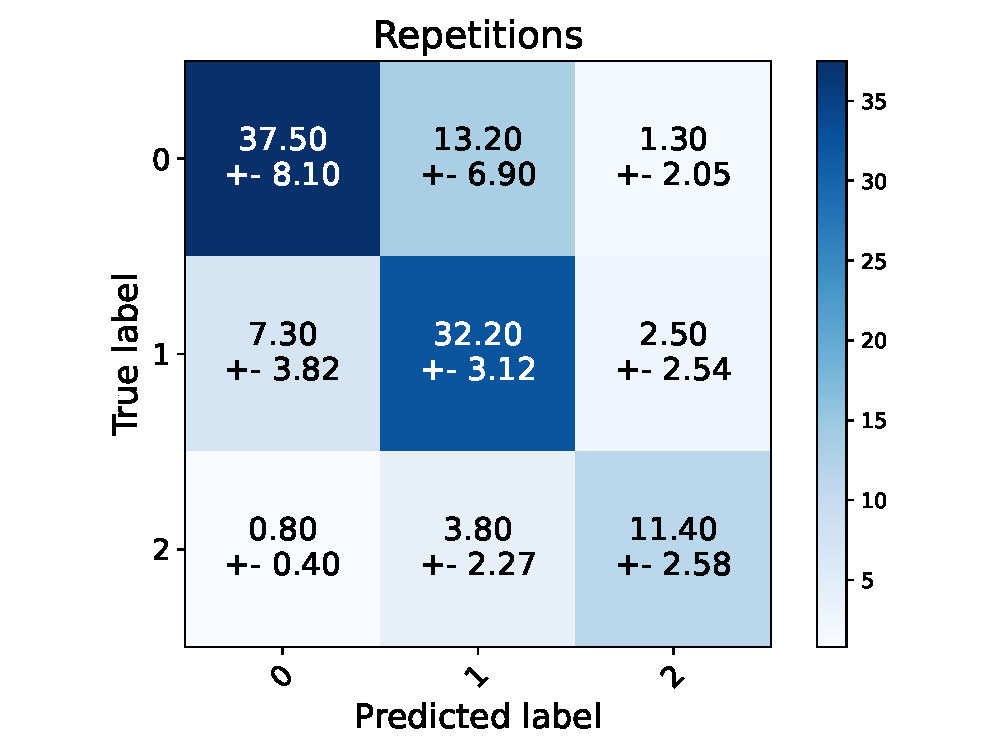
\includegraphics[width=\textwidth]{files/figs/res/trunk/cnf-reps.eps}
      \caption{}
      \label{fig:trunk-cnf-reps}
  \end{subfigure}
  ~
  \begin{subfigure}[t]{0.48\textwidth}
      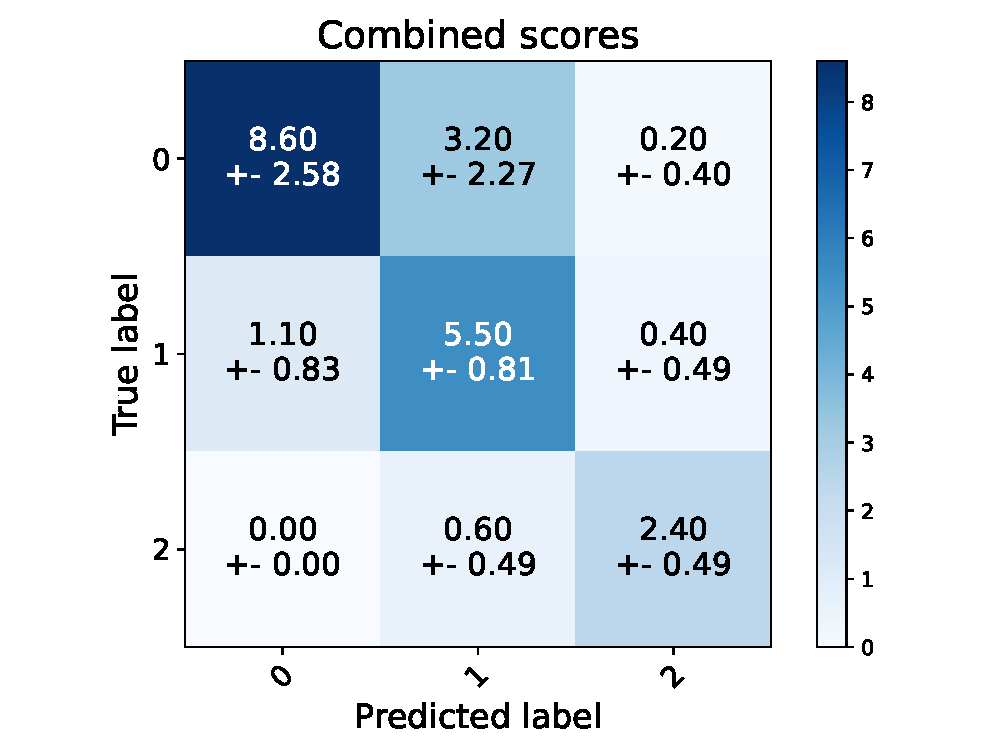
\includegraphics[width=\textwidth]{files/figs/res/trunk/cnf-combined.eps}
      \caption{}
      \label{fig:trunk-cnf-comb}
  \end{subfigure}

  \begin{subfigure}[t]{0.48\textwidth}
      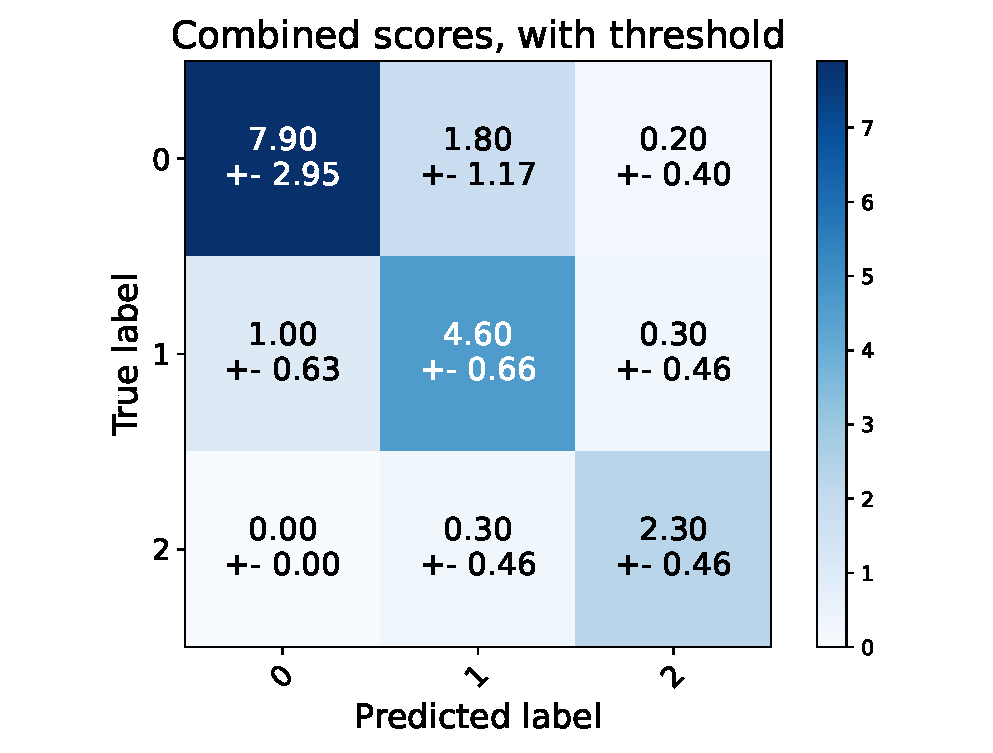
\includegraphics[width=\textwidth]{files/figs/res/trunk/cnf-combined-th.eps}
      \caption{}
      \label{fig:trunk-cnf-comb-th}
  \end{subfigure}
  ~
  \begin{subfigure}[t]{0.48\textwidth}
      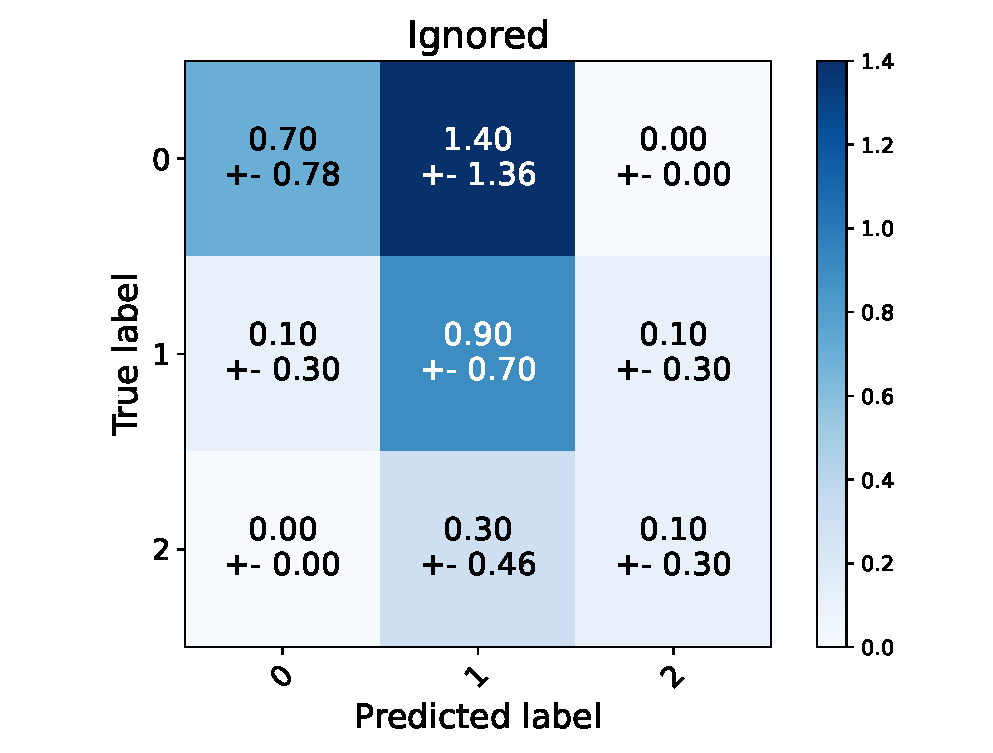
\includegraphics[width=\textwidth]{files/figs/res/trunk/cnf-ignored.eps}
      \caption{}
      \label{fig:trunk-cnf-ignored}
  \end{subfigure}
  \caption{Confusion matrices for the trunk classification on the test set. Classification of the individual repetitions is shown in (a), the combined score for the sequences of 5 repetitions is shown in (b). (c) shows the combined score with the threshold suggested in Section \ref{sec:met-combined}, i.e. all scores with a predicted probability higher than 0.4. The scores ignored due to this threshold are shown in (d). The entries in the matrices show the mean and standard deviation of the 10 ensembles trained in the cross validation.}
  \label{fig:trunk-cnfs}
\end{figure}

\begin{table}[h]
  \caption{The class distribution in the test data for the trunk POE.}
  \label{tab:trunk-class-dist}
  \centering
  \begin{tabu}[c]{cccc}
    \textbf{Class}            & 0, Good & 1, Fair & 2, Poor \\ \hline \hline
    \textbf{Proportion (\%)}  & 47.3 & 38.2 & 14.5
  \end{tabu}
\end{table}


\begin{figure}
  \centering
  \begin{subfigure}[t]{0.4\textwidth}
    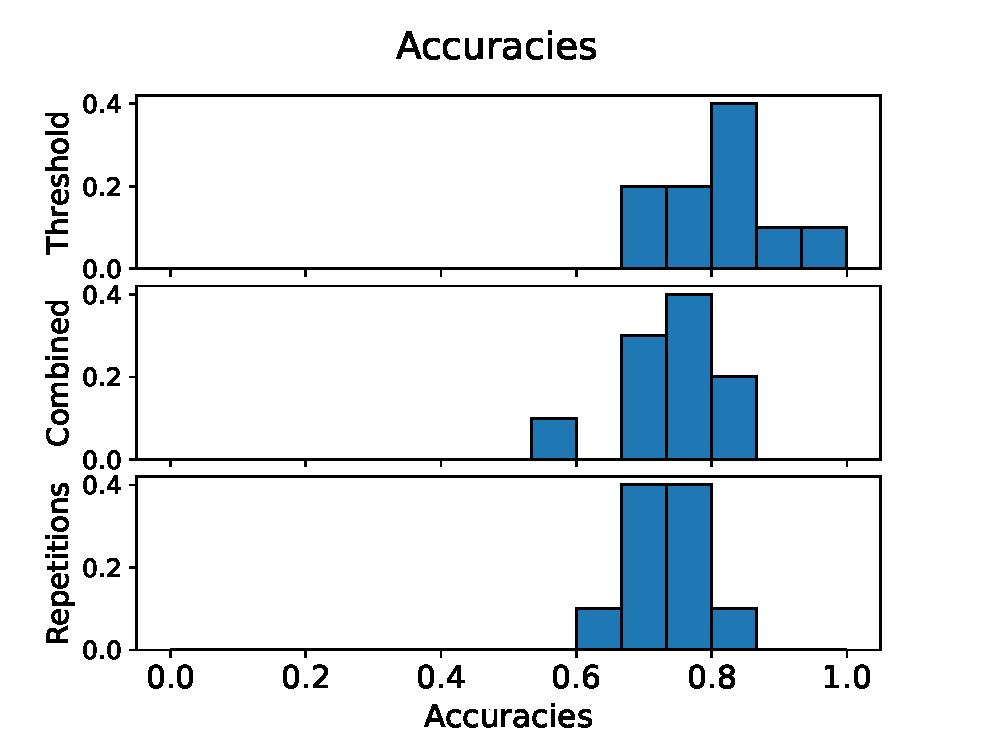
\includegraphics[width=\textwidth]{files/figs/res/trunk/acc.eps}
    \caption{}
    \label{fig:trunk-acc}
  \end{subfigure}
  ~
  \begin{subfigure}[t]{0.4\textwidth}
    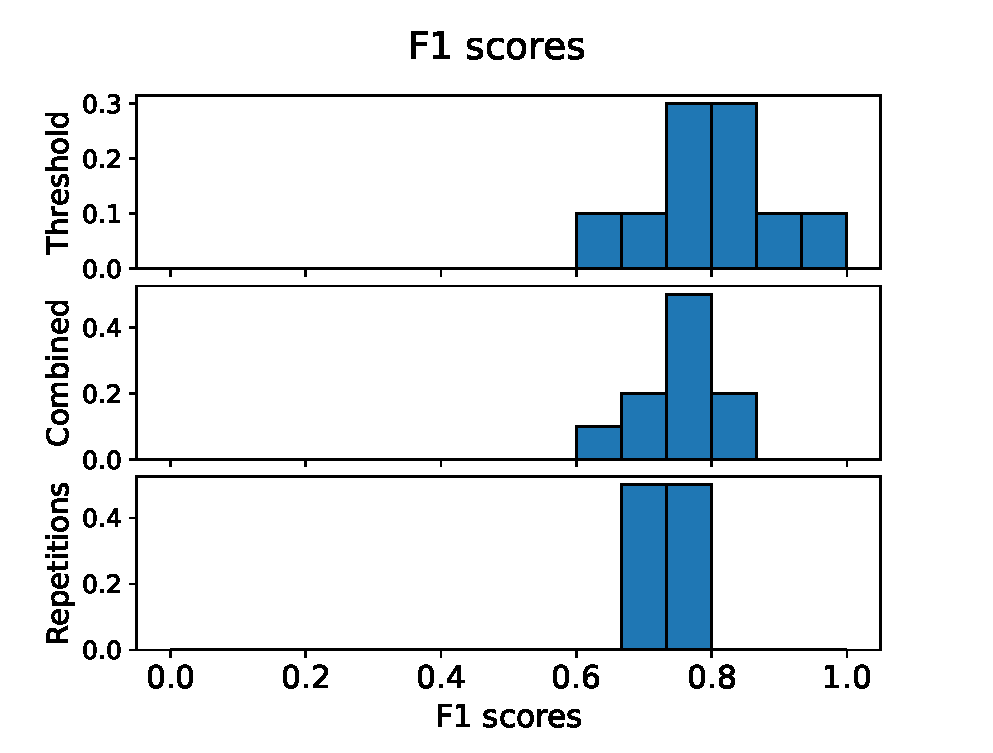
\includegraphics[width=\textwidth]{files/figs/res/trunk/f1.eps}
    \caption{}
    \label{fig:trunk-f1}
  \end{subfigure}

  \begin{subfigure}[t]{0.4\textwidth}
    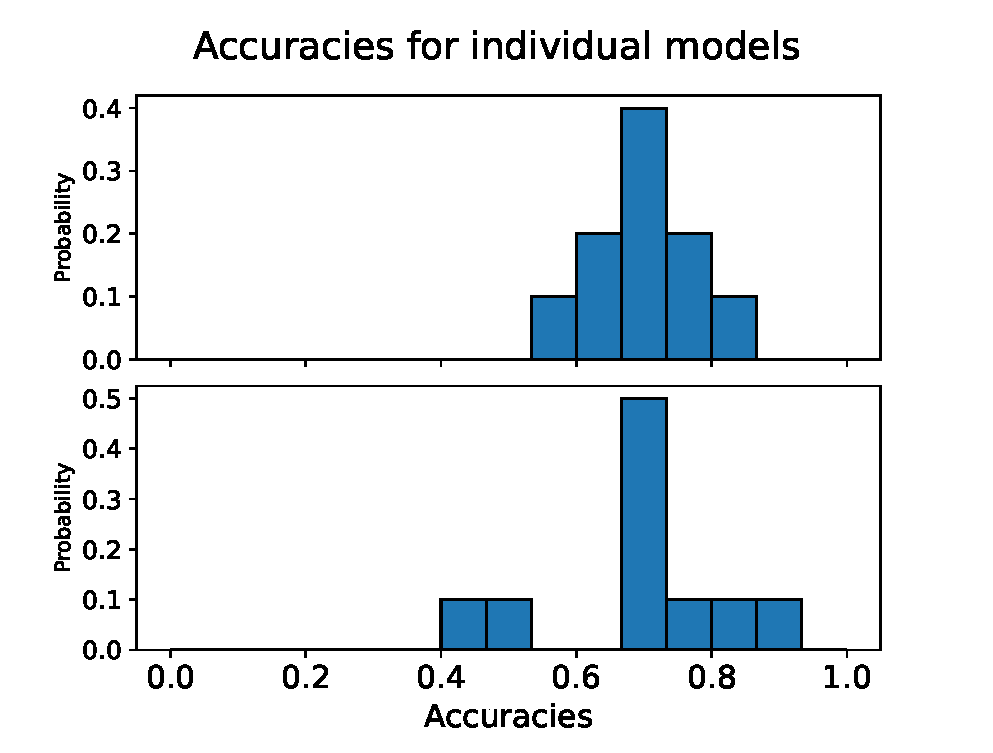
\includegraphics[width=\textwidth]{files/figs/res/trunk/acc-ind.eps}
    \caption{}
    \label{fig:trunk-acc-ind}
  \end{subfigure}
  ~
  \begin{subfigure}[t]{0.4\textwidth}
    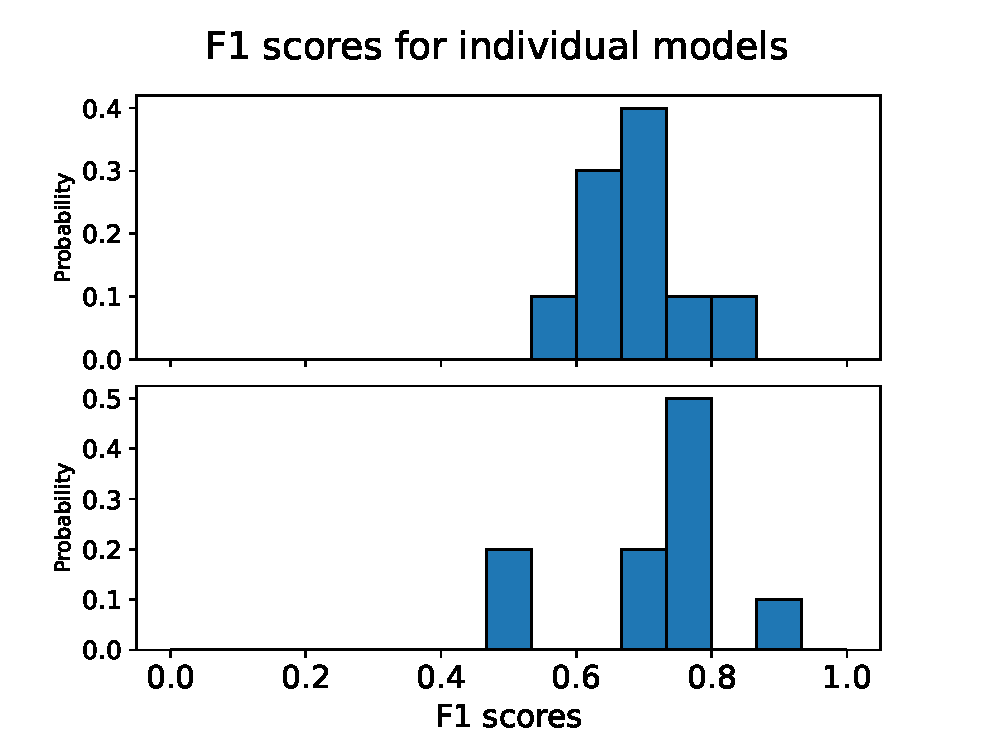
\includegraphics[width=\textwidth]{files/figs/res/trunk/f1-ind.eps}
    \caption{}
    \label{fig:trunk-f1-ind}
  \end{subfigure}
  \caption{Histograms of the accuracies and F1 scores summarized in Table \ref{tab:trunk-results} along with the same metrics for the repetition classification for the models making up the ensembles, presented in Table \ref{tab:ensemble-models}. The high precision models only predicting one class are excluded.}
  \label{fig:trunk-hist-results}
\end{figure}

Based on what is presented in Figures \ref{fig:trunk-cnfs} and \ref{fig:trunk-hist-results} as well as Table \ref{tab:trunk-results}, it seems like the performance of the classifier is enhanced by the measures taken. Table \ref{tab:trunk-improvements} shows this is true with different confidence. Neither the combined score nor the use of an ensemble can be said to improve the performance significantly, but the combined score for the five repetitions is not primarily done to improve the performance, instead this is the way the scoring system is designed. Regarding the ensemble it might be difficult to say how big of an improvement it is based on these metrics, but it reduces the variability in the results. By introducing the threshold, ignoring predictions with a predicted probability lower than 0.4, an average of 3.6 sequences are overlooked. Of these 1.7 were correctly classified and 1.9 were incorrect. %As the compute increases linearly with the number of models used this becomes

From Figure \ref{fig:trunk-cnfs} and Table~\ref{tab:trunk-class-dist} it is clear that the majority of misclassifications are between the classes 0 and 1. This is a natural effect of there being more 0s and 1s than 2s in the test set. Also, asking the experts working with this assessment system these classes are generally the ones difficult to tell apart. Another sign that the model to some extent aligns with the assessments made by the human is the better performance for the sequences where the human expert were certain about the class, seen in Table \ref{tab:trunk-results}.

\begin{table}
  \caption{With what confidence different measures led to improvements, i.e, a higher number means we can be more certain that the performance is increased by performing the corresponding measure. Calculated assuming normal distributions and using pairwise comparisons for the folds. When comparing the ensemble with the individual models the best model is chosen.}
  \label{tab:trunk-improvements}
  \centering
  \begin{tabu}[c]{|c|c|c|c|}
    \hline
    & \multicolumn{1}{c|}{\begin{tabular}[c]{@{}c@{}}\textbf{Ensemble -}\\\textbf{individual} \\\textbf{models}\end{tabular}} &
    \multicolumn{1}{c|}{\begin{tabular}[c]{@{}c@{}}\textbf{Combined -}\\\textbf{Repetitions}\end{tabular}} &
    \multicolumn{1}{c|}{\begin{tabular}[c]{@{}c@{}}\textbf{Threshold -}\\\textbf{Combined}\end{tabular}} \\ \hline
    \textbf{Accuracy} & 85\% & 75\% & 95\% \\ \hline
    \textbf{F1 score} & 75\% & 85\% & 95\% \\ \hline
  \end{tabu}
\end{table}


\begin{figure}
  \centering
  \begin{subfigure}[t]{0.33\textwidth}
    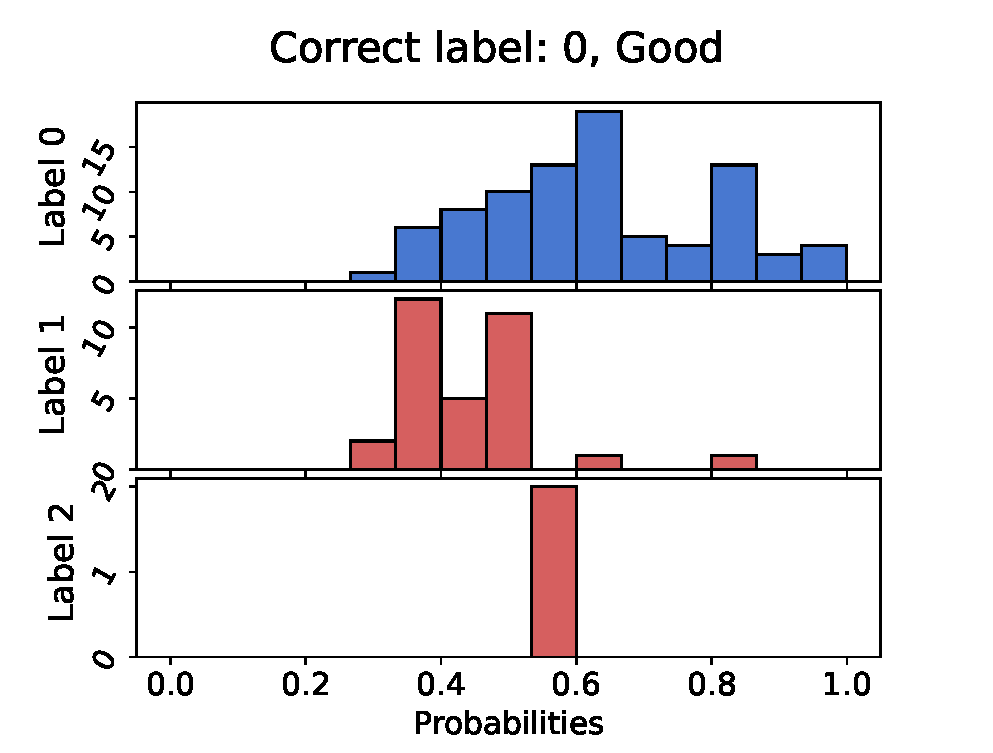
\includegraphics[width=\textwidth]{files/figs/res/trunk/pc0-rb.eps}
    \caption{}
    \label{fig:trunk-pc0}
  \end{subfigure}%
  \begin{subfigure}[t]{0.33\textwidth}
    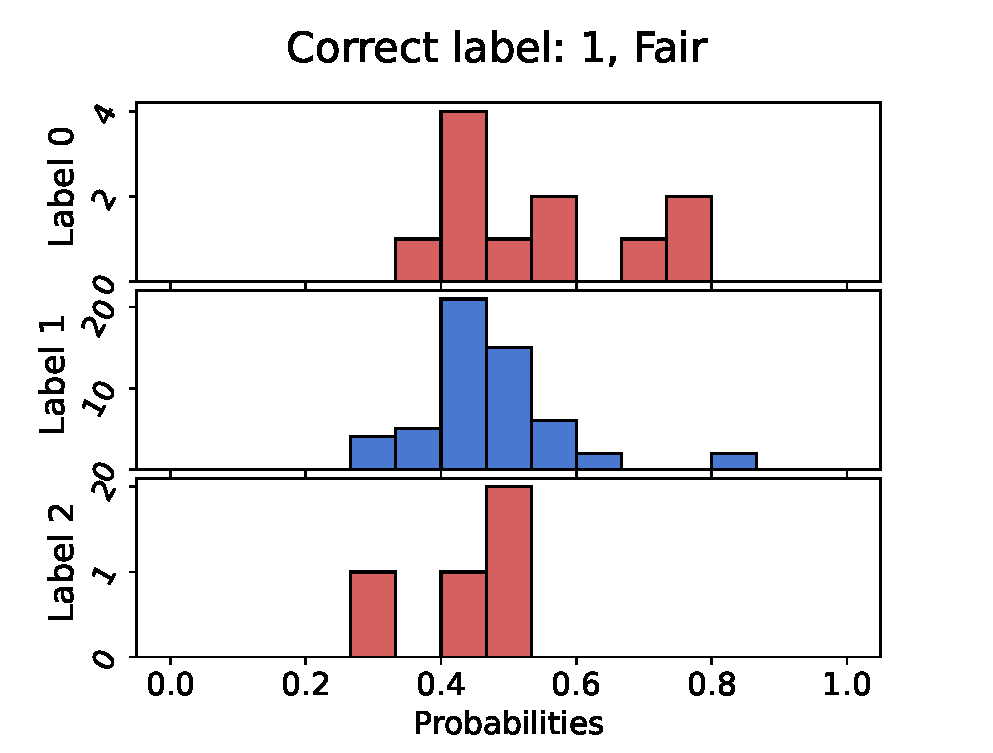
\includegraphics[width=\textwidth]{files/figs/res/trunk/pc1-rb.eps}
    \caption{}
    \label{fig:trunk-pc1}
  \end{subfigure}%
  \begin{subfigure}[t]{0.33\textwidth}
    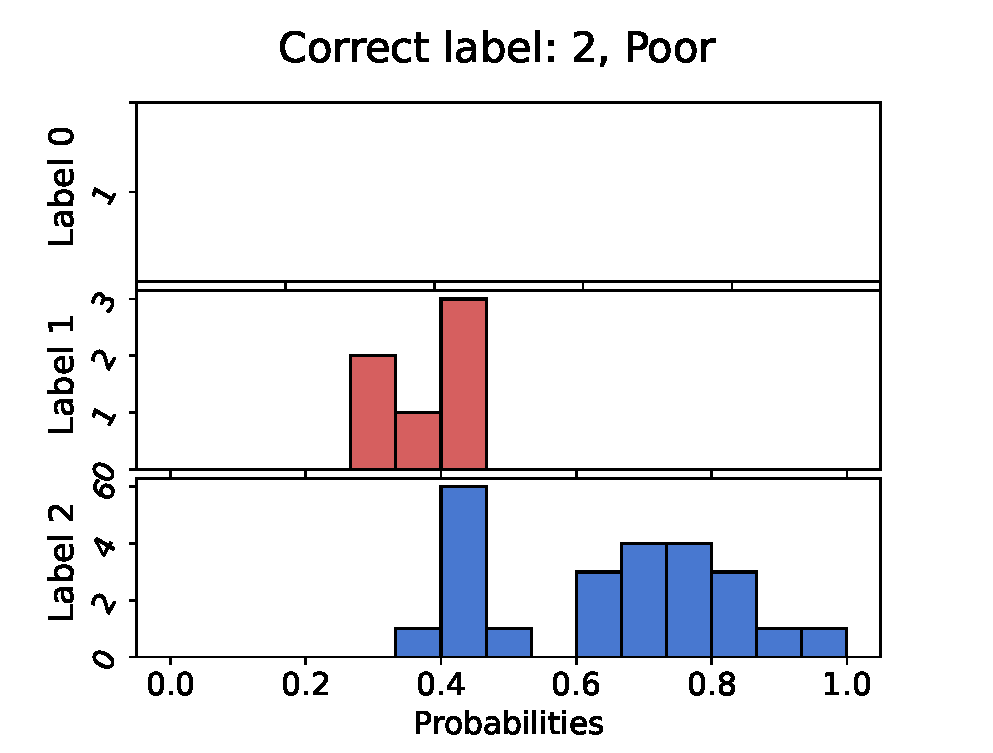
\includegraphics[width=\textwidth]{files/figs/res/trunk/pc2-rb.eps}
    \caption{}
    \label{fig:trunk-pc2}
  \end{subfigure}

  \caption{Figures showing the probabilities for the predicted class, i.e., the argmax of the model output, without threshold, for correct class 0: (a), 1: (b), and 2: (c). Incorrect predictions are shown in red.}
  \label{fig:trunk-pc}
\end{figure}

In the results above, a threshold to ignore uncertain classifications and thereby increase the performance was used. What can be seen as an extension to such a threshold, and something important for clinical use, would be to provide a confidence in the classification. Figure \ref{fig:trunk-pc} shows the probabilities for the predicted class depending on which the correct class actually is. This is the output the threshold acts on, ignoring any sample with a probability lower than 0.4. As suggested in the figure, this measure could be a suitable metric to use as prediction confidence, with the model rarely predicting incorrectly when it outputs a high class probability. However, although the ensemble weights has been adjusted as discussed in Section \ref{sec:met-ensembles}, the probabilities for class 1 is generally low.

\FloatBarrier
\subsection{Pelvis}
As in the previous section, the pelvis results are presented in Table \ref{tab:pelvis-results}, showing the accuracies, F1 scores, recall, and precisions, and in the confusion matrices in Figure \ref{fig:pelvis-cnfs}.
Along with this, histograms showing the effect of the ensemble, combined score, and threshold can be seen in Figure \ref{fig:pelvis-hist-results} and these effects are also summarized in Table \ref{tab:pelvis-improvements}. The class distribution in the test set is presented in Table~\ref{tab:pelvis-class-dist}.

\begin{table}[h]
  \centering
  \caption{Results of the ensemble for the pelvis POE. Rep., Comb., and Thresh. represents the results for the repetitions, combinations, and combinations with thresholds, respectively. The Certainties columns show the results making up the Comb. column, but for the certainty levels of the expert labeling the data. These ranges from certain (0) to uncertain (2), the variable $n$ shows how many datapoints each category contains. All results are the mean from the 10 folds $\pm$ the corresponding standard deviations. F1, recall, and precision are macro averaged.}
  \label{tab:pelvis-results}
  \small
  \begin{tabu}[c]{|c|c|c|c||c|c|c|}
    \hline
    % & \multirow21}{*}{Repetitions} & \multirow{2}{*}{Combinations} & \multirow{2}{*}{Thresholds} &  \multirow{2}{*}\multicolumn{3}{c}{Certainties}\\
    & \multirow{2}{*}{\textbf{Rep.}} & \multirow{2}{*}{\textbf{Comb.}} & \multirow{2}{*}{\textbf{Thresh.}} & \multicolumn{3}{c|}{\textbf{Certainties}}\\ \cline{5-7}
    & & & &0($n$=14)&1($n$=7)&2($n$=1)\\ \hline
    Accuracy (\%)   &63.6$\pm$10.7&69.1$\pm$10.1&\textbf{73.3$\pm$18.9}&
                    67.9$\pm$15.0&70.0$\pm$19.6&\textbf{80.0$\pm$40.0}\\ \hline
    F1 score (\%)   &55.7$\pm$13.4&66.5$\pm$15.0&\textbf{73.6$\pm$22.3}&
                    58.0$\pm$20.1&\textbf{63.7$\pm$23.8}&31.7$\pm$17.4\\ \hline
    Recall (\%)     &57.3$\pm$12.0&75.3$\pm$14.0&\textbf{77.9$\pm$14.9}&
                    56.8$\pm$20.7&\textbf{64.6$\pm$22.8}&31.7$\pm$17.4\\ \hline
    Precision (\%)  &58.3$\pm$14.9&67.0$\pm$14.4&\textbf{74.9$\pm$23.8}&
                    62.5$\pm$19.7&\textbf{68.4$\pm$24.0}&31.7$\pm$17.4\\ \hline
  \end{tabu}
\end{table}

Overall it is clear that the performance is worse for the pelvis as compared to the other \glspl{poe}. Although the different scores are not that much lower compared to the trunk \gls{poe} they vary much more making it difficult to draw any conclusions from it. It also looks less like a normal distribution, making Table \ref{tab:pelvis-improvements} unreliable. One explanation for this behavior is that the human experts considers this \gls{poe} to be the most difficult one to assess of the four considered in work. The reason for this is that the hip rotates in several planes making it difficult to assess in 2D. This probably affects the models, both directly as a more difficult pattern to identify, which might rely on information not available in this 2D data. It might also affect the models indirectly as this suggests that the training labels can be more unreliable. The higher uncertainty can also be seen in Figure \ref{fig:pelvis-cnf-ignored} as more sequences are ignored due to the threshold, 7.6 on average in this case. The high number of ignored samples is one explanation for the higher variance in the different metrics after applying the threshold.

\begin{figure}[h]
  \centering
  \begin{subfigure}[t]{0.48\textwidth}
      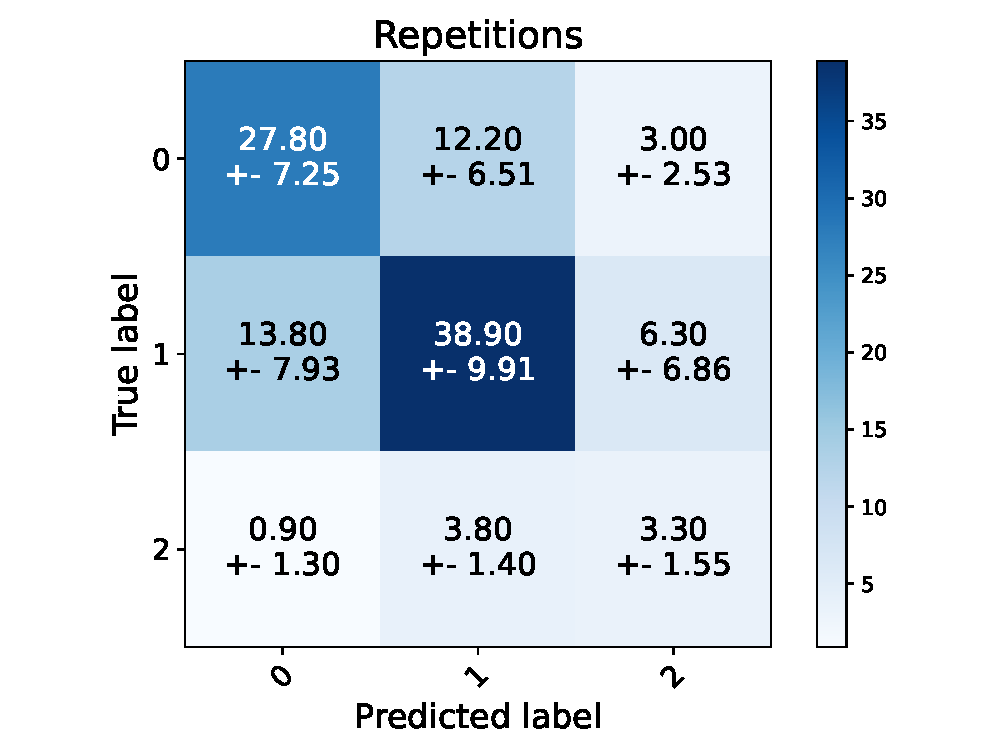
\includegraphics[width=\textwidth]{files/figs/res/pelvis/cnf-reps.eps}
      \caption{}
      \label{fig:pelvis-cnf-reps}
  \end{subfigure}
  ~
  \begin{subfigure}[t]{0.48\textwidth}
      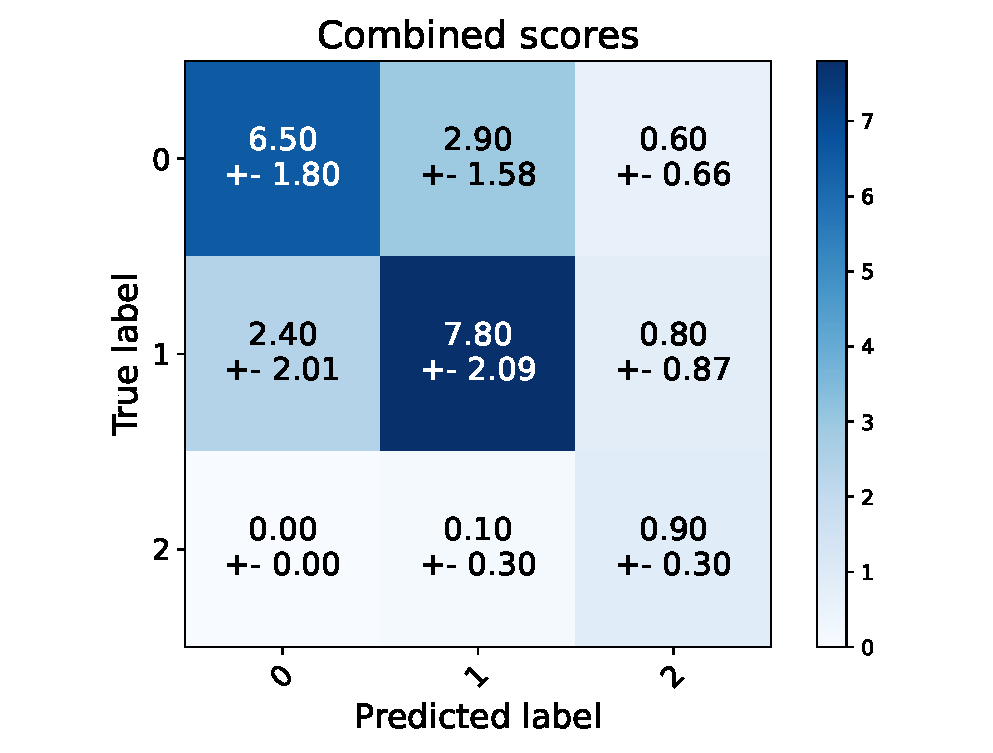
\includegraphics[width=\textwidth]{files/figs/res/pelvis/cnf-combined.eps}
      \caption{}
      \label{fig:pelvis-cnf-comb}
  \end{subfigure}

  \begin{subfigure}[t]{0.48\textwidth}
      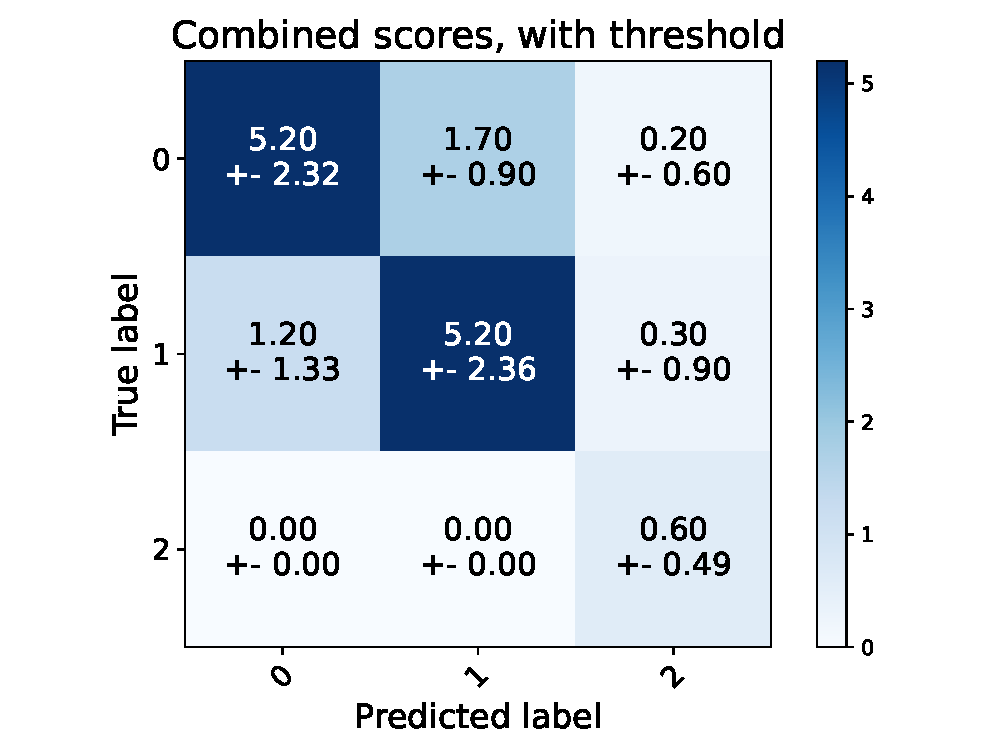
\includegraphics[width=\textwidth]{files/figs/res/pelvis/cnf-combined-th.eps}
      \caption{}
      \label{fig:pelvis-cnf-comb-th}
  \end{subfigure}
  ~
  \begin{subfigure}[t]{0.48\textwidth}
      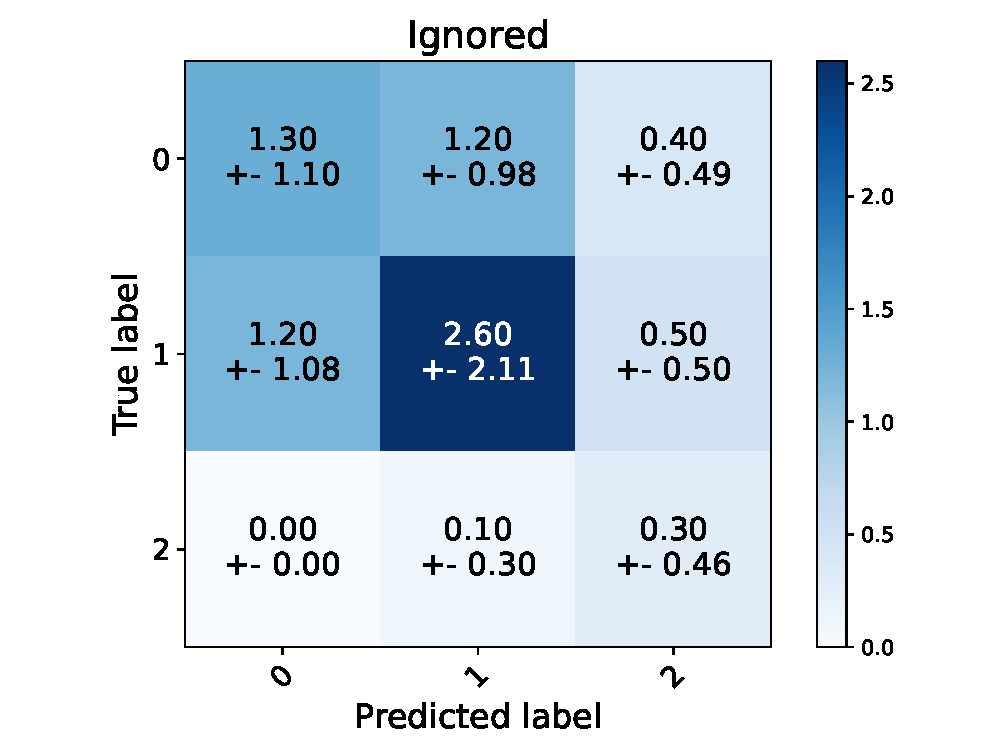
\includegraphics[width=\textwidth]{files/figs/res/pelvis/cnf-ignored.eps}
      \caption{}
      \label{fig:pelvis-cnf-ignored}
  \end{subfigure}
  \caption{Confusion matrices for the pelvis classification on the test set. Classification of the individual repetitions is shown in (a), the combined score for the sequences of 5 repetitions is shown in (b). (c) shows the combined score with the threshold suggested in Section \ref{sec:met-combined}, i.e. all scores with a predicted probability higher than 0.4. The scores ignored due to this threshold are shown in (d). The entries in the matrices show the mean and standard deviation of the 10 ensembles trained in the cross validation.}
  \label{fig:pelvis-cnfs}
\end{figure}

\begin{table}[h]
  \caption{The class distribution in the test data for the pelvis POE.}
  \label{tab:pelvis-class-dist}
  \centering
  \begin{tabu}[c]{cccc}
    \textbf{Class}            & 0, Good & 1, Fair & 2, Poor \\ \hline \hline
    \textbf{Proportion (\%)}  & 39.1 & 53.6 & 7.3
  \end{tabu}
\end{table}

\begin{figure}
  \centering
  \begin{subfigure}[t]{0.4\textwidth}
    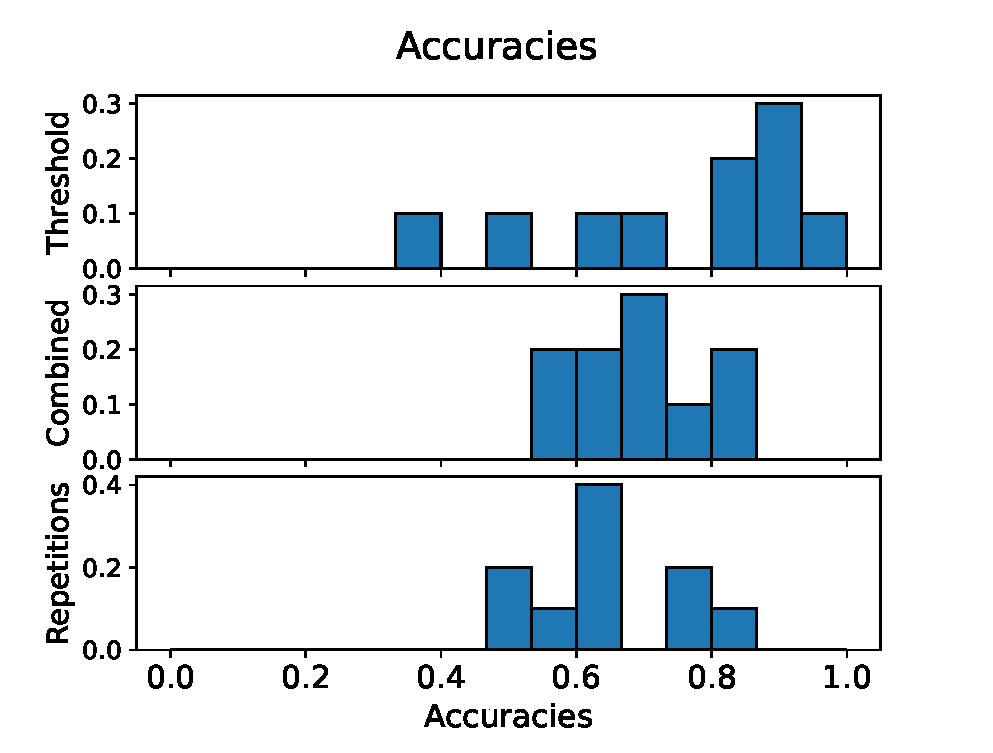
\includegraphics[width=\textwidth]{files/figs/res/pelvis/acc.eps}
    \caption{}
    \label{fig:pelvis-acc}
  \end{subfigure}
  ~
  \begin{subfigure}[t]{0.4\textwidth}
    \includegraphics[width=\textwidth]{files/figs/res/pelvis/f1.eps}
    \caption{}
    \label{fig:pelvis-f1}
  \end{subfigure}

  \begin{subfigure}[t]{0.4\textwidth}
    \includegraphics[width=\textwidth]{files/figs/res/pelvis/acc-ind.eps}
    \caption{}
    \label{fig:pelvis-acc-ind}
  \end{subfigure}
  ~
  \begin{subfigure}[t]{0.4\textwidth}
    \includegraphics[width=\textwidth]{files/figs/res/pelvis/f1-ind.eps}
    \caption{}
    \label{fig:pelvis-f1-ind}
  \end{subfigure}
  \caption{Histograms of the accuracies and F1 scores summarized in Table \ref{tab:pelvis-results} along with the same metrics for the repetition classification for the models making up the ensembles, presented in Table \ref{tab:ensemble-models}. The high precision models only predicting one class are excluded.}
  \label{fig:pelvis-hist-results}
\end{figure}

\begin{table}
  \caption{With what confidence different measures led to improvements, i.e, a higher number means we can be more certain that the performance is increased by performing the corresponding measure. Calculated assuming normal distributions and using pairwise comparisons for the folds. When comparing the ensemble with the individual models the best model is chosen.}
  \label{tab:pelvis-improvements}
  \centering
  \begin{tabu}[c]{|c|c|c|c|}
    \hline
    & \multicolumn{1}{c|}{\begin{tabular}[c]{@{}c@{}}\textbf{Ensemble -}\\\textbf{individual} \\\textbf{models}\end{tabular}} &
    \multicolumn{1}{c|}{\begin{tabular}[c]{@{}c@{}}\textbf{Combined -}\\\textbf{Repetitions}\end{tabular}} &
    \multicolumn{1}{c|}{\begin{tabular}[c]{@{}c@{}}\textbf{Threshold -}\\\textbf{Combined}\end{tabular}} \\ \hline
    \textbf{Accuracy} & - & 95\% & 85\% \\ \hline
    \textbf{F1 score} & - & 95\% & 95\% \\ \hline
  \end{tabu}
\end{table}


\begin{figure}
  \centering
  \begin{subfigure}[t]{0.33\textwidth}
    \includegraphics[width=\textwidth]{files/figs/res/pelvis/pc0-rb.eps}
    \caption{}
    \label{fig:pelvis-pc0}
  \end{subfigure}%
  \begin{subfigure}[t]{0.33\textwidth}
    \includegraphics[width=\textwidth]{files/figs/res/pelvis/pc1-rb.eps}
    \caption{}
    \label{fig:pelvis-pc1}
  \end{subfigure}%
  \begin{subfigure}[t]{0.33\textwidth}
    \includegraphics[width=\textwidth]{files/figs/res/pelvis/pc2-rb.eps}
    \caption{}
    \label{fig:pelvis-pc2}
  \end{subfigure}

  \caption{Figures showing the probabilities for the predicted class, i.e., the argmax of the model output, without threshold, for correct class 0: (a), 1: (b), and 2: (c). Incorrect predictions are shown in red.}
  \label{fig:pelvis-pc}
\end{figure}


\FloatBarrier
\subsection{Femoral Valgus}
The results for the femoral valgus \gls{poe} can be found in Figures \ref{fig:femval-cnfs}, \ref{fig:femval-hist-results}, and \ref{fig:femval-pc} as well as in Tables \ref{tab:femval-results} and \ref{tab:femval-improvements}.
This model performs well, but it seems to be slightly biased, at least for this data, towards class 1. To some extent, this can be explained by the class distribution, found in Table~\ref{tab:femval-class-dist}. On average 2.2 samples are ignored because of the threshold and 1.1 of these were correct. Notable is that it classifies a class 2 as a 0 three times and none of these are ignored due to the threshold. As can be seen in Figure~\ref{fig:femval-pc}, two of these have a probability right above the threshold of 0.4.

\begin{table}[h]
  \centering
  \caption{Results of the ensemble for the femoral valgus POE. Rep., Comb., and Thresh. represents the results for the repetitions, combinations, and combinations with thresholds, respectively. The Certainties columns show the results making up the Comb. column, but for the certainty levels of the expert labeling the data. These ranges from certain (0) to uncertain (2), the variable $n$ shows how many datapoints each category contains. All results are the mean from the 10 folds $\pm$ the corresponding standard deviations. F1, recall, and precision are macro averaged.}
  \label{tab:femval-results}
  \small
    \begin{tabu}[c]{|c|c|c|c||c|c|c|}
      \hline
      & \multirow{2}{*}{\textbf{Rep.}} & \multirow{2}{*}{\textbf{Comb.}} & \multirow{2}{*}{\textbf{Thresh.}} & \multicolumn{3}{c|}{\textbf{Certainties}}\\ \cline{5-7}
      & & & &0($n$=15)&1($n$=7)&2($n$=0)\\ \hline
      Accuracy (\%)   &69.6$\pm$6.8&79.1$\pm$9.3&\textbf{82.3$\pm$6.0}&\textbf{82.7$\pm$9.5}&71.4$\pm$11.0&-\\ \hline
      F1 score (\%)   &69.0$\pm$6.6&77.6$\pm$8.6&\textbf{81.0$\pm$5.2}&\textbf{80.8$\pm$8.6}&70.1$\pm$9.4&-\\ \hline
      Recall (\%)     &68.4$\pm$6.3&76.3$\pm$8.1&\textbf{79.5$\pm$5.5}&\textbf{80.4$\pm$7.4}&71.1$\pm$9.5&-\\ \hline
      Precision (\%)  &74.0$\pm$7.4&83.8$\pm$7.4&\textbf{86.5$\pm$5.6}&\textbf{85.2$\pm$7.6}&81.8$\pm$6.6&-\\ \hline
    \end{tabu}
\end{table}

Clearly, the performance is improved by the calculating the combined score and applying the threshold. For this \gls{poe}, the variance is also decreased by introducing the threshold, which was not the case for trunk, pelvis, nor \gls{kmfp}. As can be seen in Table~\ref{tab:femval-improvements}, the ensemble is not improving the performance, but it gives a more robust model neglecting the poor performance which can be seen in Figures \ref{fig:femval-acc-ind} and \ref{fig:femval-f1-ind} for the individual models for one of the folds.

\begin{table}[H]
  \caption{The class distribution in the test data for the femoral valgus POE.}
  \label{tab:femval-class-dist}
  \centering
  \begin{tabu}[c]{cccc}
    \textbf{Class}            & 0, Good & 1, Fair & 2, Poor \\ \hline \hline
    \textbf{Proportion (\%)}  & 32.7 & 40.0 & 27.3
  \end{tabu}
\end{table}

\begin{figure}[H]
  \centering
  \begin{subfigure}[t]{0.48\textwidth}
      \includegraphics[width=\textwidth]{files/figs/res/femval/cnf-reps.eps}
      \caption{}
      \label{fig:femval-cnf-reps}
  \end{subfigure}
  ~
  \begin{subfigure}[t]{0.48\textwidth}
      \includegraphics[width=\textwidth]{files/figs/res/femval/cnf-combined.eps}
      \caption{}
      \label{fig:femval-cnf-comb}
  \end{subfigure}

  \begin{subfigure}[t]{0.48\textwidth}
      \includegraphics[width=\textwidth]{files/figs/res/femval/cnf-combined-th.eps}
      \caption{}
      \label{fig:femval-cnf-comb-th}
  \end{subfigure}
  ~
  \begin{subfigure}[t]{0.48\textwidth}
      \includegraphics[width=\textwidth]{files/figs/res/femval/cnf-ignored.eps}
      \caption{}
      \label{fig:femval-cnf-ignored}
  \end{subfigure}
  \caption{Confusion matrices for the femoral valgus classification on the test set. Classification of the individual repetitions is shown in (a), the combined score for the sequences of 5 repetitions is shown in (b). (c) shows the combined score with the threshold suggested in Section \ref{sec:met-combined}, i.e. all scores with a predicted probability higher than 0.4. The scores ignored due to this threshold are shown in (d). The entries in the matrices show the mean and standard deviation of the 10 ensembles trained in the cross validation.}
  \label{fig:femval-cnfs}
\end{figure}

\begin{table}[h]
  \caption{With what confidence different measures led to improvements, i.e, a higher number means we can be more certain that the performance is increased by performing the corresponding measure. Calculated assuming normal distributions and using pairwise comparisons for the folds. When comparing the ensemble with the individual models the best model is chosen.}
  \label{tab:femval-improvements}
  \centering
  \begin{tabu}[c]{|c|c|c|c|}
    \hline
    & \multicolumn{1}{c|}{\begin{tabular}[c]{@{}c@{}}\textbf{Ensemble -}\\\textbf{individual} \\\textbf{models}\end{tabular}} &
    \multicolumn{1}{c|}{\begin{tabular}[c]{@{}c@{}}\textbf{Combined -}\\\textbf{Repetitions}\end{tabular}} &
    \multicolumn{1}{c|}{\begin{tabular}[c]{@{}c@{}}\textbf{Threshold -}\\\textbf{Combined}\end{tabular}} \\ \hline
    \textbf{Accuracy} & - & 95\% & 95\% \\ \hline
    \textbf{F1 score} & - & 95\% & 95\% \\ \hline
  \end{tabu}
\end{table}

\begin{figure}
  \centering
  \begin{subfigure}[t]{0.4\textwidth}
    \includegraphics[width=\textwidth]{files/figs/res/femval/acc.eps}
    \caption{}
    \label{fig:femval-acc}
  \end{subfigure}
  ~
  \begin{subfigure}[t]{0.4\textwidth}
    \includegraphics[width=\textwidth]{files/figs/res/femval/f1.eps}
    \caption{}
    \label{fig:femval-f1}
  \end{subfigure}

  \begin{subfigure}[t]{0.4\textwidth}
    \includegraphics[width=\textwidth]{files/figs/res/femval/acc-ind.eps}
    \caption{}
    \label{fig:femval-acc-ind}
  \end{subfigure}
  ~
  \begin{subfigure}[t]{0.4\textwidth}
    \includegraphics[width=\textwidth]{files/figs/res/femval/f1-ind.eps}
    \caption{}
    \label{fig:femval-f1-ind}
  \end{subfigure}
  \caption{Histograms of the accuracies and F1 scores summarized in Table \ref{tab:femval-results} along with the same metrics for the repetition classification for the models making up the ensembles, presented in Table \ref{tab:ensemble-models}. The high precision models only predicting one class are excluded.}
  \label{fig:femval-hist-results}
\end{figure}

% LAGG TILL FIGURE MED GRAD CAM!!!!!!

\begin{figure}
  \centering
  \begin{subfigure}[t]{0.33\textwidth}
    \includegraphics[width=\textwidth]{files/figs/res/femval/pc0-rb.eps}
    \caption{}
    \label{fig:femval-pc0}
  \end{subfigure}%
  \begin{subfigure}[t]{0.33\textwidth}
    \includegraphics[width=\textwidth]{files/figs/res/femval/pc1-rb.eps}
    \caption{}
    \label{fig:femval-pc1}
  \end{subfigure}%
  \begin{subfigure}[t]{0.33\textwidth}
    \includegraphics[width=\textwidth]{files/figs/res/femval/pc2-rb.eps}
    \caption{}
    \label{fig:femval-pc2}
  \end{subfigure}

  \caption{Figures showing the probabilities for the predicted class, i.e., the argmax of the model output, without threshold, for correct class 0: (a), 1: (b), and 2: (c). Incorrect predictions are shown in red.}
  \label{fig:femval-pc}
\end{figure}

As for the trunk model, the probability for class one is low. This is clearly not a problem for the classification, as mentioned above this model seems to be slightly biased towards class 1. It is however something to consider for the confidence score desirable in a clinical setting.


With the ensemble consisting of different models, some of the explainability from the X-InceptionTime architecture is lost. It is still possible to get importance values for each time step, but the regular models will not differentiate between the inputs. Figure~\ref{fig:gradcam} shows the activation maps for some different inputs to a single X-InceptionTime model, both for correctly and incorrectly classified samples. It can be seen how the same regions seems to be deemed important for the same predictions.%, but the importance is slightly higher when the prediction is correct.

\begin{figure}[h]
  \begin{subfigure}[t]{0.32\textwidth}
    \includegraphics[width=\textwidth]{files/figs/res/femval/gradcam/00.eps}
    \caption{}
    \label{fig:femval-00}
  \end{subfigure}
  ~
  \begin{subfigure}[t]{0.32\textwidth}
    \includegraphics[width=\textwidth]{files/figs/res/femval/gradcam/11.eps}
    \caption{}
    \label{fig:femval-11}
  \end{subfigure}
  ~
  \begin{subfigure}[t]{0.32\textwidth}
    \includegraphics[width=\textwidth]{files/figs/res/femval/gradcam/22.eps}
    \caption{}
    \label{fig:femval-22}
  \end{subfigure}

  \begin{subfigure}[t]{0.32\textwidth}
    \includegraphics[width=\textwidth]{files/figs/res/femval/gradcam/10.eps}
    \caption{}
    \label{fig:femval-10}
  \end{subfigure}
  ~
  \begin{subfigure}[t]{0.32\textwidth}
    \includegraphics[width=\textwidth]{files/figs/res/femval/gradcam/01.eps}
    \caption{}
    \label{fig:femval-01}
  \end{subfigure}
  ~
  \begin{subfigure}[t]{0.32\textwidth}
    \includegraphics[width=\textwidth]{files/figs/res/femval/gradcam/12.eps}
    \caption{}
    \label{fig:femval-12}
  \end{subfigure}
  \caption{Activation maps applied to different inputs showing what was important for decision. The subplots show from the top: $y$ coordinate of the right shoulder, $x$ coordinate of the right hip, $x$ coordinate of the right knee, and angle between right knee and right ankle.}
  \label{fig:gradcam}
\end{figure}




\FloatBarrier
\subsection{Knee Medial-to-Foot Position}
As can be seen in Table~\ref{tab:kmfp-class-dist}, the \gls{kmfp} data is heavily unbalanced making it somewhat difficult to analyze. As long as this training set is a representable class distribution this model might perform satisfactory. However, it has seen very few examples of both class 1 and 2, so the risk of out-of-distribution samples if deploying this model is probably rather high. Regarding the performance metrics this model achieves a good accuracy which is natural since it will do so by just classifying most data as class 0. Based on the other metrics and the confusion matrices it becomes clear that it does not simply do this. To avoid such behavior some of the models used in the ensemble were slightly biased towards class 1 and 2. This shows in the result mainly as a low precision for class 1 compared to the other \glspl{poe}. The low standard deviation for the accuracy shows that the number of misclassification is similar for all examples. Due to the macro averaging of the other metrics together with the class imbalance, variations in a single classification of class 1 or 2 results in the large standard deviations seen for F1, recall, and precision.

%The threshold results in an average of 0.7 ignored sequences for this \gls{poe}.
% can be seen that it performs somewhat in line with
% The high variance in the F1 score is explained by the imbalanced data as any misclassification of class 1 or 2 will have a big effect on this. For this \gls{poe} an average of 0.7 sequences are ignored due to the threshold and 0.5 of these was correctly classified.

\begin{figure}[h]
  \centering
  \begin{subfigure}[t]{0.48\textwidth}
      \includegraphics[width=\textwidth]{files/figs/res/kmfp/cnf-reps.eps}
      \caption{}
      \label{fig:kmfp-cnf-reps}
  \end{subfigure}
  ~
  \begin{subfigure}[t]{0.48\textwidth}
      \includegraphics[width=\textwidth]{files/figs/res/kmfp/cnf-combined.eps}
      \caption{}
      \label{fig:kmfp-cnf-comb}
  \end{subfigure}

  \begin{subfigure}[t]{0.48\textwidth}
      \includegraphics[width=\textwidth]{files/figs/res/kmfp/cnf-combined-th.eps}
      \caption{}
      \label{fig:kmfp-cnf-comb-th}
  \end{subfigure}
  ~
  \begin{subfigure}[t]{0.48\textwidth}
      \includegraphics[width=\textwidth]{files/figs/res/kmfp/cnf-ignored.eps}
      \caption{}
      \label{fig:kmfp-cnf-ignored}
  \end{subfigure}
  \caption{Confusion matrices for the KMFP classification on the test set. Classification of the individual repetitions is shown in (a), the combined score for the sequences of 5 repetitions is shown in (b). (c) shows the combined score with the threshold suggested in Section \ref{sec:met-combined}, i.e. all scores with a predicted probability higher than 0.4. The scores ignored due to this threshold are shown in (d). The entries in the matrices show the mean and standard deviation of the 10 ensembles trained in the cross validation.}
  \label{fig:kmfp-cnfs}
\end{figure}

\begin{table}[h]
  \caption{The class distribution in the test data for the KMFP POE.}
  \label{tab:kmfp-class-dist}
  \centering
  \begin{tabu}[c]{cccc}
    % \hline
    \textbf{Class}      & 0, Good & 1, Fair & 2, Poor \\ \hline \hline
    \textbf{Proportion (\%)} & 78.2 & 17.3 & 4.5 \\ %\hline
  \end{tabu}
\end{table}

\begin{table}
  \centering
  \caption{Results of the ensemble for the KMFP POE. Rep., Comb., and Thresh. represents the results for the repetitions, combinations, and combinations with thresholds, respectively. The Certainties columns show the results making up the Comb. column, but for the certainty levels of the expert labeling the data. These ranges from certain (0) to uncertain (2), the variable $n$ shows how many datapoints each category contains. All results are the mean from the 10 folds $\pm$ the corresponding standard deviations. F1, recall, and precision are macro averaged.}
  \label{tab:kmfp-results}
  \small
    \begin{tabu}[c]{|c|c|c|c||c|c|c|}
      \hline
      & \multirow{2}{*}{\textbf{Rep.}} & \multirow{2}{*}{\textbf{Comb.}} & \multirow{2}{*}{\textbf{Thresh.}} & \multicolumn{3}{c|}{\textbf{Certainties}}\\ \cline{5-7}
      & & & &0($n$=19)&1($n$=2)&2($n$=1)\\ \hline
      Accuracy (\%)   &82.3$\pm$3.1&89.5$\pm$4.5&\textbf{90.3$\pm$4.3}
                      &\textbf{92.6$\pm$5.3}&90.0$\pm$20.0&30.0$\pm$45.8\\ \hline
      F1 score (\%)   &65.1$\pm$13.7&69.0$\pm$24.6&\textbf{74.0$\pm$22.3}
                      &\textbf{69.3$\pm$28.6}&57.8$\pm$17.8&10.0$\pm$15.3\\ \hline
      Recall (\%)     &63.8$\pm$14.4&75.9$\pm$26.7&\textbf{81.1$\pm$24.7}
                      &\textbf{75.3$\pm$29.4}&60.0$\pm$13.3&10.0$\pm$15.3\\ \hline
      Precision (\%)  &\textbf{78.5$\pm$8.2}&66.1$\pm$24.0&71.4$\pm$22.6
                      &\textbf{67.2$\pm$28.9}&56.7$\pm$20.0&10.0$\pm$15.2\\ \hline
    \end{tabu}
\end{table}


\begin{figure}
  \centering
  \begin{subfigure}[t]{0.4\textwidth}
    \includegraphics[width=\textwidth]{files/figs/res/kmfp/acc.eps}
    \caption{}
    \label{fig:kmfp-acc}
  \end{subfigure}
  ~
  \begin{subfigure}[t]{0.4\textwidth}
    \includegraphics[width=\textwidth]{files/figs/res/kmfp/f1.eps}
    \caption{}
    \label{fig:kmfp-f1}
  \end{subfigure}

  \begin{subfigure}[t]{0.4\textwidth}
    \includegraphics[width=\textwidth]{files/figs/res/kmfp/acc-ind.eps}
    \caption{}
    \label{fig:kmfp-acc-ind}
  \end{subfigure}
  ~
  \begin{subfigure}[t]{0.4\textwidth}
    \includegraphics[width=\textwidth]{files/figs/res/kmfp/f1-ind.eps}
    \caption{}
    \label{fig:kmfp-f1-ind}
  \end{subfigure}
  \caption{Histograms of the accuracies and F1 scores summarized in Table \ref{tab:kmfp-results} along with the same metrics for the repetition classification for the models making up the ensembles, presented in Table \ref{tab:ensemble-models}. The high precision models only predicting one class are excluded.}
  \label{fig:kmfp-hist-results}
\end{figure}


\begin{table}
  \caption{With what confidence different measures led to improvements, i.e, a higher number means we can be more certain that the performance is increased by performing the corresponding measure. Calculated assuming normal distributions and using pairwise comparisons for the folds. When comparing the ensemble with the individual models the best model is chosen.}
  \label{tab:kmfp-improvements}
  \centering
  \begin{tabu}[c]{|c|c|c|c|}
    \hline
    & \multicolumn{1}{c|}{\begin{tabular}[c]{@{}c@{}}\textbf{Ensemble -}\\\textbf{individual} \\\textbf{models}\end{tabular}} &
    \multicolumn{1}{c|}{\begin{tabular}[c]{@{}c@{}}\textbf{Combined -}\\\textbf{Repetitions}\end{tabular}} &
    \multicolumn{1}{c|}{\begin{tabular}[c]{@{}c@{}}\textbf{Threshold -}\\\textbf{Combined}\end{tabular}} \\ \hline
    \textbf{Accuracy} & - & 95\% & 95\% \\ \hline
    \textbf{F1 score} & - & 95\% & 95\% \\ \hline
  \end{tabu}
\end{table}


\begin{figure}
  \centering
  \begin{subfigure}[t]{0.33\textwidth}
    \includegraphics[width=\textwidth]{files/figs/res/kmfp/pc0-rb.eps}
    \caption{}
    \label{fig:kmfp-pc0}
  \end{subfigure}%
  \begin{subfigure}[t]{0.33\textwidth}
    \includegraphics[width=\textwidth]{files/figs/res/kmfp/pc1-rb.eps}
    \caption{}
    \label{fig:kmfp-pc1}
  \end{subfigure}%
  \begin{subfigure}[t]{0.33\textwidth}
    \includegraphics[width=\textwidth]{files/figs/res/kmfp/pc2-rb.eps}
    \caption{}
    \label{fig:kmfp-pc2}
  \end{subfigure}

  \caption{Figures showing the probabilities for the predicted class, i.e., the argmax of the model output, without threshold, for correct class 0: (a), 1: (b), and 2: (c). Incorrect predictions are shown in red.}
  \label{fig:kmfp-pc}
\end{figure}

\FloatBarrier
\subsection{Summary}
The results with their 95\% confidence intervals are summarized in Table \ref{tab:sum-ci}. These confidence intervals assumes Gaussian distributions, which is not unrealistic for trunk, femoral valgus, and to some extent \gls{kmfp}. For the pelvis however, this assumption does not seem to be very reasonable. Based on this, it can be said that the model for femoral valgus seems to perform the best followed by trunk. \gls{kmfp} achieves a high accuracy, but it is difficult to draw any conclusions about the performance for the Fair (1) or Poor (2) classes due to the very few examples. The pelvis model does not perform very well which might be due to that it is based on information not available in the 2D joint position data. For all \glspl{poe} the developed models clearly outperforms the baseline methods.

The only difference between the different fold models is a slight variation in the training data. Still, the result, generated on the same testing data, clearly varies. This suggests that more data would be very welcome for all models. Both to improve the performance through bigger training sets and to give more reliable evaluations thanks to more testing data.

\begin{table}[h]
  \caption{Approximative 95\% confidence intervals for the performance of the combined scores with thresholds for different POEs, assuming Gaussian distributions. }
  \label{tab:sum-ci}
  \centering
  \begin{tabu}[c]{|c|c|c|c|c|}
    \hline
    & \textbf{Trunk} & \textbf{Pelvis} &\textbf{Femoral Valgus} & \textbf{\gls{kmfp}} \\ \hline
    \textbf{Accuracy (\%)}  & 80.0$\pm$4.9 & 73.3$\pm$11.9 & 82.3$\pm$3.8 & \textbf{90.3$\pm$2.7} \\\hline
    \textbf{F1 score (\%)}  & 79.9$\pm$5.6 & 73.6$\pm$14.1 & \textbf{81.0$\pm$3.3} & 74.0$\pm$14.1 \\ \hline
    \textbf{Recall (\%)}    & \textbf{81.6$\pm$4.6} & 77.9$\pm$9.4  & 79.5$\pm$3.5 & 81.1$\pm$15.6 \\ \hline
    \textbf{Precision (\%)} & 83.0$\pm$4.3 & 74.9$\pm$15.1 & \textbf{86.5$\pm$3.5} & 71.4$\pm$14.3 \\\hline
  \end{tabu}
\end{table}

Regarding the model selection, it is notable that padded and normalized data yields similar results. This suggests that, at least with this amount of data, the frequency content or the speed of the movements is not an indicator of the \gls{poe} score. Instead, the overall shape of the movements of the different body parts are important, which matches the descriptions in Appendix~\ref{app:poe-task}. Normalizing the data length probably unifies these shapes slightly over all data, which might make it easier to find patterns.

Another thing to note is that deep models does not seem to be effective as models with depths of one and two performed the best. Similarly, the InceptionTime model where interactions between the inputs are taken into account does not perform significantly better than X-InceptionTime. This suggests, at least with this amount of data, that the discriminating features are not that complicated and does not depend on direct interactions between the inputs, apart from difference or angles in some cases. With more data this might be different as new patterns could be found.

% !TEX root=../../mt-motion-analysis.tex
\chapter{Conclusions and Discussion} \label{ch:conclusions}

}


% \fontsize{9}{9}
{\setstretch{0.8}
% {\footnotesize

\printbibliography
\addcontentsline{toc}{chapter}{References}}
% }
% !TEX root=../../mt-motion-analysis.tex
\newpage
\appendix
\newpage
\etocdepthtag.toc{mtappendix}
\etocsettagdepth{mtchapter}{none}
\etocsettagdepth{mtappendix}{subsection}
\etoctocstyle{1}{Appendix - Contents}
\tableofcontents
\newpage


\chapter{POEs}
\begin{figure}[b]
  \centering
  \includegraphics[height=\textheight]{files/figs/poes-detailed-rot.png}
  % \caption{}
  \label{}
\end{figure}


\chapter{wtf}
this is the information

% \chapter{Histograms over probabilities on validation sets}
\section{Femoral Valgus}
\begin{figure}
  \begin{subfigure}[t]{0.3\textwidth}
    \includegraphics[width=\textwidth]{files/figs/app/hists/femval/r0.png}
  \end{subfigure}
  ~
  \begin{subfigure}[t]{0.3\textwidth}
    \includegraphics[width=\textwidth]{files/figs/app/hists/femval/r1.png}
  \end{subfigure}
  ~
  \begin{subfigure}[t]{0.3\textwidth}
    \includegraphics[width=\textwidth]{files/figs/app/hists/femval/r2.png}
  \end{subfigure}

  \begin{subfigure}[t]{0.3\textwidth}
    \includegraphics[width=\textwidth]{files/figs/app/hists/femval/pr0.png}
  \end{subfigure}
  ~
  \begin{subfigure}[t]{0.3\textwidth}
    \includegraphics[width=\textwidth]{files/figs/app/hists/femval/pr1.png}
  \end{subfigure}
  ~
  \begin{subfigure}[t]{0.3\textwidth}
    \includegraphics[width=\textwidth]{files/figs/app/hists/femval/pr2.png}
  \end{subfigure}

  \begin{subfigure}[t]{0.3\textwidth}
    \includegraphics[width=\textwidth]{files/figs/app/hists/femval/c0.png}
  \end{subfigure}
  ~
  \begin{subfigure}[t]{0.3\textwidth}
    \includegraphics[width=\textwidth]{files/figs/app/hists/femval/c1.png}
  \end{subfigure}
  ~
  \begin{subfigure}[t]{0.3\textwidth}
    \includegraphics[width=\textwidth]{files/figs/app/hists/femval/c2.png}
  \end{subfigure}

  \begin{subfigure}[t]{0.3\textwidth}
    \includegraphics[width=\textwidth]{files/figs/app/hists/femval/pc0.png}
  \end{subfigure}
  ~
  \begin{subfigure}[t]{0.3\textwidth}
    \includegraphics[width=\textwidth]{files/figs/app/hists/femval/pc1.png}
  \end{subfigure}
  ~
  \begin{subfigure}[t]{0.3\textwidth}
    \includegraphics[width=\textwidth]{files/figs/app/hists/femval/pc2.png}
  \end{subfigure}
\end{figure}


\end{document}
